\documentclass[10pt,a4paper]{article}

%\documentclass[10pt,onecolumn,letterpaper]{IEEEtran}

\usepackage{setspace}
%\AtBeginDocument{\setstretch{.9}}
%\doublespacing  % doublespacing is done after title and before abstract

\usepackage{caption}
\usepackage{subcaption}
\usepackage[title]{appendix}

%\usepackage[margin=0.25in]{geometry}

%\usepackage{lineno}
%\linenumbers

\usepackage{fullpage}
\usepackage{authblk}
\usepackage[utf8]{inputenc}
\usepackage{amsmath,bm}
\usepackage{amsthm}
\usepackage{amssymb}
\usepackage{hyperref}
\usepackage{adjustbox}
\usepackage{multirow}
\usepackage{graphicx}
\usepackage{booktabs}
\usepackage{caption}
\usepackage{subcaption}
\usepackage[table]{xcolor}
\usepackage{tabu}
\usepackage{subcaption}
\usepackage{longtable}
\usepackage{amssymb}
\usepackage{footnote}
\usepackage{hyperref}
\usepackage{multirow}
\usepackage{comment}
\usepackage{cite}
\usepackage{threeparttable}
\usepackage{makecell}
\usepackage{mathtools} % for multiline-multicase equation
\usepackage{float}
\usepackage{array}
\usepackage{tabularx} % in the preamble
\usepackage{tikz}
\usepackage{ulem}
\usepackage{algorithm2e}

\usepackage{tabularx}
\newcolumntype{Y}{>{\centering\arraybackslash}X}
\newcolumntype{C}[1]{>{\centering\arraybackslash}m{#1}}

% \usepackage[demo]{graphicx}
% \usepackage[utf8]{inputenc}
% \usepackage{subfigure}
\usepackage{xcolor}
\newcommand{\add}[1]{{\color{blue} #1}}
\newcommand{\addb}[1]{{\color{red} #1}}
\newcommand{\SR}[1]{{\color{red} #1}}
\newcommand{\methodname}{{\color{purple}Method\_Name~}}

\newtheorem{theorem}{Theorem}[section]
\newtheorem{corollary}{Corollary}[theorem]
\newtheorem{lemma}[theorem]{Lemma}

\renewcommand{\thetheorem}{\arabic{theorem}}  % to start numbering from 1

%\usepackage{booktabs, caption, makecell}
%\renewcommand\theadfont{\bfseries}
\usepackage{subfiles} % For subfiles
\usepackage{hyperref}
\usepackage[labelfont=bf]{caption}

\usepackage{xcolor}

\renewcommand\theadalign{bc}
\renewcommand\theadfont{\bfseries}
\renewcommand\theadgape{\Gape[4pt]}
\renewcommand\cellgape{\Gape[4pt]}



\makesavenoteenv{tabular}
\makesavenoteenv{table}

\hypersetup{
    urlcolor=blue,
}

\providecommand{\keywords}[1]{\textbf{\textit{Keywords:}} #1}

\providecommand{\runningtitle}[1]{\textbf{\textit{Running title:}} #1}


\title{QT-WEAVER: Correcting quartet distribution improves phylogenomic analyses despite gene tree estimation error
\author[1,*]{Navid Bin Hasan$^{1,\dag}$, Sohaib$^{1,\dag}$, and Md. Shamsuzzoha Bayzid}
}

\affil[1]{Department of Computer Science and Engineering\protect \\
Bangladesh University of Engineering and Technology, Dhaka-1205, Bangladesh}
% \affil[2]{Department of Computer Science\protect\\University of Maryland, College Park, Maryland 20742, USA}
%\affil[3]{Department of Computer Science and Engineering\protect\\The Ohio State University, Ohio 43210, USA}
\affil[$\dag$]{These authors contributed equally to this work}
\affil[*]{Corresponding author: shams\_bayzid@cse.buet.ac.bd}
\date{}




\begin{document}

\maketitle


\pagenumbering{gobble} % to turn of the page numbering.
%\pagenumbering{arabic}


%\doublespacing
%\newpage
\begin{abstract}
Summarizing individual gene trees into species phylogenies using coalescent-based methods has become a standard approach in phylogenomics. 
However, gene tree estimation error (GTEE) arising from a combination of reasons (ranging from analytical factors to more biological causes, as in short gene sequences) can potentially impact the accuracy of phylogenomic inference.
We, for the first time, introduce the problem of correcting the quartet distribution induced by a set of estimated gene trees, which involves updating the weights of the quartets to better reflect their relative importance within the gene tree distribution. We present QT-WEAVER, the first method of its kind, which learns the conflicts within the quartet distribution induced by a given set of gene trees and generates an updated quartet distribution by adjusting the weights accordingly. QT-WEAVER is a general-purpose technique needing no explicit modeling of the subject system or reasons for GTEE or gene tree heterogeneity. Experimental studies on a collection of simulated and empirical data sets suggest that QT-WEAVER can effectively account for GTEE, which results in a substantial improvement in the species tree accuracy. Additionally, the concept of quartet conflicts and related algorithmic and combinatorial innovations introduced in this study will benefit various quartet-based computations. Therefore, QT-WEAVER advances the state-of-the-art in species tree estimation from gene trees in the face of GTEE. QT-WEAVER is freely available in open-source form at \url{https://github.com/navidh86/QT-WEAVER}.

%quartets that is often closer to the quartet distribution of true gene trees than that of the estimated gene trees, and thereby accounting for gene tree estimation error.

%accuracy of species tree inference. 
%Remarkably, QT-GILD not only imputes the missing quartets but it can also account for gene tree estimation error.

%Remarkably, QT-GILD not only imputes the missing quartets but it can also ``correct’’ the estimated quartets -- resulting in a set of quartets that is often closer to the quartet distribution of true gene trees than that of the estimated gene trees, and thereby accounting for gene tree estimation error.  %QT-GILD -- with its auto-encoder based deep learning approach combined with concepts from NLP and the demonstrated notable improvements in tree accuracy -- significantly advances the state-of-the-art in species tree estimation from gene trees despite missing data. 


%Read this: https://academic.oup.com/mbe/article/37/5/1495/5685817?searchresult=1

%add model independence from this paper.

% needing no explicit modeling of the subject system and reasons for missing data

%Although there is a continuing effort to make models more realistic (Ronquist and Huelsenbeck 2003; Stamatakis 2014), model misspecification is and will likely be the norm rather than the exception.

%\keywords{Species tree, gene tree, incomplete lineage sorting (ILS), quartet distribution, quartet consistency, missing data, deep learning, autoencoder.}


\end{abstract}

\newcommand{\quartet}[4]{
  \begin{tikzpicture}
    % Nodes
    \node (a) at (0, 2) {};
    \node (b) at (0, 0) {};
    \node (c) at (3, 2) {};
    \node (d) at (3, 0) {};
    \node (center1) at (1, 1) {};
    \node (center2) at (2, 1) {};
    \node (name) at (1.5, -0.5) {$#1#2|#3#4$};

    % Edges
    \draw[thick] (a) -- (center1);
    \draw[thick] (b) -- (center1);
    \draw[thick] (center1) -- (center2);
    \draw[thick] (center2) -- (c);
    \draw[thick] (center2) -- (d);

    % Dots at nodes
    \fill (a) circle (2pt);
    \fill (b) circle (2pt);
    \fill (c) circle (2pt);
    \fill (d) circle (2pt);
    \fill (center1) circle (2pt);
    \fill (center2) circle (2pt);

    % Labels
    \node at (-0.2, 2) {#1};
    \node at (3.2, 2) {#3};
    \node at (3.2, 0) {#4};
    \node at (-0.2, 0) {#2};
  \end{tikzpicture}
}

\newcommand{\fivetax}[5]{
\begin{tikzpicture}
% Nodes
\node (a) at (0, 2) {};
\node (b) at (0, 0) {};
\node (c) at (3, 2) {};
\node (d) at (3, 0) {};
\node (x) at (0.5, 1.5) {};
\node (e) at (0, 1) {};

\node (center1) at (1, 1) {};
\node (center2) at (2, 1) {};

% Edges
\draw[thick] (a) -- (x);
\draw[thick] (center1) -- (x);
\draw[thick] (b) -- (center1);
\draw[thick] (center1) -- (center2);
\draw[thick] (center2) -- (c);
\draw[thick] (center2) -- (d);
\draw[thick] (e) -- (x);

% Dots at nodes
\fill (a) circle (2pt);
\fill (b) circle (2pt);
\fill (c) circle (2pt);
\fill (d) circle (2pt);
\fill (x) circle (2pt);
\fill (e) circle (2pt);
\fill (center1) circle (2pt);
\fill (center2) circle (2pt);

% Labels
\node at (-0.2, 2) {#1};
\node at (3.2, 2) {#3};
\node at (3.2, 0) {#4};
\node at (-0.2, 0) {#2};
\node at (-0.2, 1) {#5};
\end{tikzpicture}
}

\newcommand{\fivetaxcol}[5]{
\begin{tikzpicture}
% Nodes
\node (a) at (0, 2) {};
\node (b) at (0, 0) {};
\node (c) at (3, 2) {};
\node (d) at (3, 0) {};
\node (x) at (0.5, 1.5) {};
\node (e) at (0, 1) {};

\node (center1) at (1, 1) {};
\node (center2) at (2, 1) {};

% Edges
\draw[thick] (a) -- (x);
\draw[thick] (center1) -- (x);
\draw[thick] (b) -- (center1);
\draw[thick] (center1) -- (center2);
\draw[thick] (center2) -- (c);
\draw[thick] (center2) -- (d);
\draw[thick, red] (e) -- (x);


% Dots at nodes
\fill (a) circle (2pt);
\fill (b) circle (2pt);
\fill (c) circle (2pt);
\fill (d) circle (2pt);
\fill (x) circle (2pt);
% \fill[red] (e) circle (2pt);
\fill (e) circle (2pt);
\fill (center1) circle (2pt);
\fill (center2) circle (2pt);

% Labels
\node at (-0.2, 2) {#1};
\node at (3.2, 2) {#3};
\node at (3.2, 0) {#4};
\node at (-0.2, 0) {#2};
\node at (-0.2, 1) {#5};
\end{tikzpicture}
}

\newcommand{\fivetaxinv}[5]{
\begin{tikzpicture}
% Nodes
\node (a) at (0, 2) {};
\node (b) at (0, 0) {};
\node (c) at (3, 2) {};
\node (d) at (3, 0) {};
\node (x) at (0.5, 0.5) {};
\node (e) at (0, 1) {};

\node (center1) at (1, 1) {};
\node (center2) at (2, 1) {};

% Edges
\draw[thick] (a) -- (center1);
\draw[thick] (center1) -- (x);
\draw[thick] (b) -- (x);
\draw[thick] (center1) -- (center2);
\draw[thick] (center2) -- (c);
\draw[thick] (center2) -- (d);
\draw[thick] (e) -- (x);

% Dots at nodes
\fill (a) circle (2pt);
\fill (b) circle (2pt);
\fill (c) circle (2pt);
\fill (d) circle (2pt);
\fill (x) circle (2pt);
\fill (e) circle (2pt);

\fill (center1) circle (2pt);
\fill (center2) circle (2pt);

% Labels
\node at (-0.2, 2) {#1};
\node at (3.2, 2) {#3};
\node at (3.2, 0) {#4};
\node at (-0.2, 0) {#2};
\node at (-0.2, 1) {#5};
\end{tikzpicture}
}

\newcommand{\fivetaxmult}[5]{
\begin{tikzpicture}
% Nodes
\node (a) at (0, 2) {};
\node (b) at (0, 0) {};
\node (c) at (3, 2) {};
\node (d) at (3, 0) {};
\node (x) at (2.5, 0.5) {};
\node (x2) at (2.5, 1.5) {};
\node (x3) at (1.5, 1) {};
\node (y) at (0.5, 1.5) {};
\node (e) at (3, 1) {};
\node (e2) at (2, 2) {};
\node (e3) at (1.5, 0) {};

\node (center1) at (1, 1) {};
\node (center2) at (2, 1) {};

% Edges
\draw[thick] (a) -- (center1);
\draw[thick] (center1) -- (b);
% \draw[thick] (b) -- (x);
\draw[thick] (center1) -- (center2);
\draw[thick] (center2) -- (c);
\draw[thick] (center2) -- (d);

\draw[thick, dotted, red, shorten <=-1mm, shorten >=-1mm] (e) -- (x);
\draw[thick, dotted, red, shorten <=-1mm, shorten >=-1mm] (e2) -- (x2);
\draw[thick, dotted, red, shorten <=-1mm, shorten >=-1mm] (e3) -- (x3);


% Dots at nodes
\fill (a) circle (2pt);
\fill (b) circle (2pt);
\fill (c) circle (2pt);
\fill (d) circle (2pt);
% \fill (x) circle (2pt);
\fill (e) circle (2pt);
\fill (e2) circle (2pt);
\fill (e3) circle (2pt);
\fill (center1) circle (2pt);
\fill (center2) circle (2pt);

% Labels
\node at (-0.2, 2) {#1};
\node at (3.2, 2) {#3};
\node at (3.2, 0) {#4};
\node at (-0.2, 0) {#2};
\node at (3.2, 1) {#5};
\node at (1.8, 2) {#5};
\node at (1.7, 0) {#5};
\end{tikzpicture}
}







\newcommand{\fivetaxdccol}[5]{
\begin{tikzpicture}
% Nodes
\node (a) at (0, 2) {};
\node (b) at (0, 0) {};
\node (c) at (3, 2) {};
\node (d) at (3, 0) {};
\node (x) at (2.5, 0.5) {};
\node (x2) at (2.5, 1.5) {};
\node (x3) at (1.5, 1) {};
\node (y) at (0.5, 1.5) {};
\node (e) at (3, 1) {};
\node (e2) at (2, 2) {};
\node (e3) at (1.5, 0) {};

\node (center1) at (1, 1) {};
\node (center2) at (2, 1) {};

% Edges
\draw[thick] (a) -- (center1);
\draw[thick] (center1) -- (b);
% \draw[thick] (b) -- (x);
\draw[thick] (center1) -- (center2);
\draw[thick] (center2) -- (c);
\draw[thick] (center2) -- (x);
\draw[thick] (x) -- (d);

\draw[thick, red] (e) -- (x);



% Dots at nodes
\fill (a) circle (2pt);
\fill (b) circle (2pt);
\fill (c) circle (2pt);
\fill (d) circle (2pt);
% \fill (x) circle (2pt);
% \fill[red] (e) circle (2pt);
\fill (e) circle (2pt);
\fill (center1) circle (2pt);
\fill (center2) circle (2pt);
\fill (x) circle (2pt);

% Labels
\node at (-0.2, 2) {#1};
\node at (3.2, 2) {#3};
\node at (3.2, 0) {#4};
\node at (-0.2, 0) {#2};
\node at (3.2, 1) {#5};
% \node at (1.8, 2) {#5};
% \node at (1.7, 0) {#5};
\end{tikzpicture}
}

\newcommand{\fivetaxdc}[5]{
\begin{tikzpicture}
% Nodes
\node (a) at (0, 2) {};
\node (b) at (0, 0) {};
\node (c) at (3, 2) {};
\node (d) at (3, 0) {};
\node (x) at (2.5, 0.5) {};
\node (x2) at (2.5, 1.5) {};
\node (x3) at (1.5, 1) {};
\node (y) at (0.5, 1.5) {};
\node (e) at (3, 1) {};
\node (e2) at (2, 2) {};
\node (e3) at (1.5, 0) {};

\node (center1) at (1, 1) {};
\node (center2) at (2, 1) {};

% Edges
\draw[thick] (a) -- (center1);
\draw[thick] (center1) -- (b);
% \draw[thick] (b) -- (x);
\draw[thick] (center1) -- (center2);
\draw[thick] (center2) -- (c);
\draw[thick] (center2) -- (x);
\draw[thick] (x) -- (d);

\draw[thick, shorten <=-1mm, shorten >=-1mm] (e) -- (x);



% Dots at nodes
\fill (a) circle (2pt);
\fill (b) circle (2pt);
\fill (c) circle (2pt);
\fill (d) circle (2pt);
% \fill (x) circle (2pt);
\fill (e) circle (2pt);
\fill (center1) circle (2pt);
\fill (center2) circle (2pt);
\fill (x) circle (2pt);

% Labels
\node at (-0.2, 2) {#1};
\node at (3.2, 2) {#3};
\node at (3.2, 0) {#4};
\node at (-0.2, 0) {#2};
\node at (3.2, 1) {#5};
% \node at (1.8, 2) {#5};
% \node at (1.7, 0) {#5};
\end{tikzpicture}
}


\newcommand{\triplet}[4]{
\begin{tikzpicture}
% Nodes
\node (a) at (0, 2) {};
\node (b) at (0, 0) {};
\node (center1) at (1, 1) {};
\node (c) at (2.5, 1) {};
\node (x) at (0.5, 0.5) {};
\node (y) at (0.5, 1.5) {};
\node (z) at (1.75, 1) {};
\node (d1) at (0, 1) {};
\node (d2) at (1, 2) {};
\node (d3) at (1.75, 0) {};

% Edges
\draw[thick] (a) -- (center1);
\draw[thick] (center1) -- (b);
\draw[thick] (center1) -- (c);

\draw[thick, dotted, red, shorten <=-1mm, shorten >=-1mm] (d1) -- (x);
\draw[thick, dotted, red, shorten <=-1mm, shorten >=-1mm] (d2) -- (y);
\draw[thick, dotted, red, shorten <=-1mm, shorten >=-1mm] (d3) -- (z);


% Dots at nodes
\fill (a) circle (2pt);
\fill (b) circle (2pt);
\fill (c) circle (2pt);
\fill (d1) circle (2pt);
\fill (d2) circle (2pt);
\fill (d3) circle (2pt);
\fill (center1) circle (2pt);

% Labels
\node at (-0.2, 2) {#1};
\node at (2.7, 1) {#3};
\node at (-0.2, 1) {#4};
\node at (1.2, 2) {#4};
\node at (1.95, 0) {#4};
\node at (-0.2, 0) {#2};
% \node at (3.2, 1) {#5};
% \node at (1.8, 2) {#5};
% \node at (1.7, 0) {#5};
\end{tikzpicture}
}


\newcommand{\linequart}[6]{
\begin{tikzpicture}
% Nodes
\node (a) at (0, 0) {};
\node (b) at (6, 0) {};
\node (cx) at (1.2, 0) {};
\node (xx) at (2.4, 0) {};
\node (dx) at (3.6, 0) {};
\node (yx) at (4.8, 0) {};

\node (c) at (1.2, 1) {};
\node (d) at (3.6, 1) {};
\node (x) at (2.4, -1) {};
\node (y) at (4.8, -1) {};

% Edges
\draw[thick] (a) -- (b);
\draw[dashed] (c) -- (cx);
\draw[dashed] (d) -- (dx);
\draw[dashed] (x) -- (xx);
\draw[dashed] (y) -- (yx);

% Dots at nodes
\fill (a) circle (2pt);
\fill (b) circle (2pt);
\fill (cx) circle (1.2pt);
\fill (dx) circle (1.2pt);
\fill (xx) circle (1.2pt);
\fill (yx) circle (1.2pt);
\fill (c) circle (1.5pt);
\fill (d) circle (1.5pt);
\fill (x) circle (1.5pt);
\fill (y) circle (1.5pt);

% Labels
\node at (-0.2, 0) {#1};
\node at (6.2, 0) {#2};
\node at (1, 1) {#3};
\node at (3.4, 1) {#4};
\node at (2.6, -1) {#5};
\node at (5, -1) {#6};

\end{tikzpicture}
}
\clearpage
\pagenumbering{arabic}

%\newpage
\section{Introduction}

Species tree estimation from genes sampled across the whole genome has become routine with the advent of high-throughput sequencing technologies, generating genome-wide datasets that include hundreds or even thousands of loci. Species tree estimation from multiple genes is commonly done through concatenation (also known as ``combined analysis''), which combines sequence alignments from different loci into a single supermatrix and then computes a tree on the supermatrix. While concatenation can produce accurate species trees when gene trees are concordant, it can be statistically inconsistent~\cite{roch2015likelihood,consensus-inconsistent}, and produce incorrect trees with high support~\cite{kubatko-degnan-2007} when gene trees differ from the species tree due to various biological processes such as incomplete lineage sorting (ILS), gene duplication and loss (GDL), horizontal gene transfer (HGT), etc. As a result, summary methods~\cite{mpest,astral,larget-bioinf2010,glass,stem,svdquartet,steac,njst,wqfm,astrid,stelar} that combine estimated gene trees while explicitly accounting for gene tree discordance have drawn substantial interest among systematists. However, summary methods are susceptible to gene tree estimation errors (GTEE), which can arise from various reasons including short gene sequences, inaccurate alignments, and the limitations of the models and algorithms used for inferring gene trees from sequence data. 


Due to the growing awareness that GTEE is a major contributor to inaccuracies of summary methods, there has been great interest in developing tools~\cite{notung,treefix,rasmussen2011bayesian,traction,profilenj,tt,treefix-dtl-bansal2015improved,nguyen2012accounting,jacox2017resolution,lafond2017gene} to account for GTEE for improved species tree estimations. Most of these methods are species tree aware as they use a reference species tree in addition to the input gene trees. These species tree aware  methods essentially reconcile/modify gene trees to make them closer in distance to the species tree by minimizing a species tree aware cost function. However, gene trees could be discordant and are not always expected to closely match the species tree. %such as Robinson Foulds distance,  inferred evolutionary events (GDL), etc., 
%even when the true gene and species trees are discordant. 
Additionally, ``integrative'' methods such as ProfileNJ and TreeFix use available sequence data as well as the estimated gene trees and reference species trees. Obtaining a reasonably accurate reference species tree despite substantial amounts of GTEE is difficult and the inaccuracy in the reference tree may have cascading effects on gene tree corrections. More importantly, species tree aware methods, specifically TreeFix and TRACTION, have been criticized for their potential to increase GTEE where gene trees are discordant with species trees~\cite{zhiyan}. Bayesian techniques for co-estimating both gene trees and species trees such as BEST~\cite{best}, *BEAST~\cite{heled-drummond}, and PHYLDOG~\cite{boussau2013genome} 
can produce substantially more accurate gene and species trees than other methods, but are not scalable to genome-level analyses~\cite{bayzid2013naive,smith2013target,bayzid-incomplete,leache-rannala,szollHosi2015inference}.
Therefore, despite significant attempts to account for GTEE, substantial challenges remain.



%\add{
%Gene Tree Estimation Error(GTEE) is a well-studied problem in the field of phylogenetics. The limited amount of sequence data available for each gene makes the construction of gene trees susceptible to errors. These estimation errors can propagate to the species tree, as gene tree data is a primary input for species tree estimation. Consequently, errors in gene tree estimation are a major contributor to inaccuracies in species tree estimation. This challenge has led to the development of many different methods aimed at reducing errors in gene tree estimation. However, despite these advances, each method has its limitations, and the challenge of accurate gene tree estimation remains. 

%Species tree attraction-based approaches aim to reconcile gene trees, making them more consistent with the species tree. Two prominent methods in this category are TreeFix~\cite{treefix} and TRACTION~\cite{traction}. However, the evolutionary history of genes often diverges from species phylogeny due to processes such as Incomplete Lineage Sorting (ILS), Gene Duplication and Loss (GDL), and Horizontal Gene Transfer (HGT). Consequently, gene trees are not always expected to closely match the species tree. Both methods, TreeFix and TRACTION, have been criticized for increasing Gene Tree Estimation Error (GTEE) in datasets where gene trees are genuinely discordant with species trees (Zhi Yan et al.~\cite{zhiyan}). These methods are effective when uncorrected GTEE is high and gene tree discordance is relatively low. Nonetheless, they depend on a reference species tree to adjust gene trees, aligning them more closely with the species tree. Additionally, TreeFix requires gene sequence data to address incongruences between the species tree and the gene tree. ProfileNJ ~\cite{profilenj} corrects weakly supported branches in gene trees using a reference species tree and a distance matrix.

%Older methods, such as NOTUNG (Durand et al. 2006~\cite{notung}) and tt (Gorecki and Eulenstein 2011~\cite{tt}), are considerably simpler. These approaches focus on local rearrangements around an initial gene tree to identify an error-corrected gene tree with minimal duplication-loss cost. However, they have two primary limitations: their search space is restricted, and they tend to overfit the gene tree, making it overly similar to the species tree.

%}

% missing data
%There has been notable progress in constructing large scale phylogenetic trees by analyzing genome-wide data, but substantial challenges remain. Assembling a complete dataset with hundreds of orthologous genes from a large set of species remains a difficult task which has downstream impact in species tree inference~\cite{hosner2016avoiding,streicher2016should,xi2016impact}. Gene trees can be incomplete due to various reasons ranging from biological processes as in gene birth and loss~\cite{mgd-amb} to biases in taxon and gene sampling, stochasticity inherent in collecting data across thousands of loci, and difficulty in sequencing and assembling the complete set of taxa of interest (see \cite{hosner2016avoiding,streicher2016should,lemmon2009effect,burleigh2009inferring} for more elaborate discussion). Incomplete gene trees may decrease the species tree accuracy~\cite{bayzid-incomplete,xi2016impact,nute2018performance} and introduce ambiguity in the tree search~\cite{sanderson2011terraces,spterrace}. Indeed, as we will show in our experimental results, incomplete gene trees substantially reduce the accuracy of the best existing coalescent based summary methods.  

% We address the problem of missing data in phylogenomic data sets, for the first time, by formulating the \textit{Quartet Distribution Imputation - \add{QDI}} problem

In this study, we address the problem of GTEE in the context of species tree estimation, by formulating the \textit{Quartet Distribution Correction} (QDC) problem for the first time, where we seek to ``correct/adjust'' the distribution of quartets induced by a given set of estimated gene trees. QDC attempts to account for GTEE without resorting to any reference species tree. %or computationally intensive joint inference of species and gene phylogenies using full Bayesian inference under the multi-species coalescent (MSC) model. 
Quartet-based summary methods have drawn considerable attention because quartets (unrooted gene trees with four taxa) can avoid the ``anomaly zone''~\cite{DR06,DR09,degnan2013anomalous}, where the most likely gene tree topology may differ from the true species tree topology and can produce highly accurate species trees. ASTRAL, the most widely used summary method, infers a species tree by maximizing the number of quartets in the gene trees that are consistent with the species tree. Another class of methods (known as quartet amalgamation techniques~\cite{snir_quartets_2008,qfm,qfm-fi,wqfm,wqmc}), such as wQFM~\cite{wqfm} and wQMC~\cite{wqmc}, involves inferring weighted quartets for every group of four taxa (with weights correspond to the relative importance of the quartets) and then combining them into a single species tree. In this study, we present QT-WEAVER (\textbf{Q}uar\textbf{t}et \textbf{We}ight \textbf{A}djustment by \textbf{V}erifying, \textbf{E}stimating, and \textbf{R}ectifying quartet weights), a novel method that learns the weighted quartet distribution induced by a set of gene trees to identify and verify certain patterns of quartet conflicts and subsequently update the weights accordingly. We introduced the concept of ``quartet conflicts'' and proved key analytical and combinatorial results that underpin QT-WEAVER's ability to learn and adjust quartet distributions without relying on any reference species tree or sequence data, offering a robust approach to improving the accuracy of species tree inference. 

The quartet distributions corrected by QT-WEAVER often align more closely with the true gene tree quartets than with those from the estimated gene trees, thereby effectively accounting for GTEE. Our experimental results, based on a diverse set of simulated and real biological datasets covering a wide range of challenging model conditions, demonstrate that amalgamating QT-WEAVER's corrected quartets significantly improves species tree inference accuracy. Moreover, QT-WEAVER is a general-purpose approach that does not require explicit modeling of the reasons for gene tree heterogeneity or GTEE, making it more resilient to model misspecification. QT-WEAVER is the first of its kind which advances the state-of-the-art in species tree estimation in the presence of GTEE.

% for conclusion: QT-WEAVER obviates the need for any reference tree or computationally intensive joint inference of species and gene phylogenies using full Bayesian inference under the multi-species coalescent (MSC) model to account for GTEE.

\section{Quartet Distribution Correction Problem}
\subsection{Problem Definition}
Let $\mathcal{G} =  \{g_1, g_2, \ldots, g_k\}$ be a set of $k$ gene trees, where each $g_i$ is a tree on taxon set $S_i \subseteq S$ (i.e., any gene tree $g_i$ can be on the full set $S$ of $n$ taxa or can be on a subset $S_i$ of taxa, making the gene tree incomplete). For a set of four taxa $a,b,c,d \in S$, the quartet tree $ab|cd$ denotes the unrooted quartet tree in which the pair $a, b$ is separated from the pair $c, d$ by an edge. Note that there are three alternative quartet topologies ($ab|cd, ac|bd, ad|bc$) for four taxa.
%Note that on every set of four species, there are three possible unrooted quartet trees (simply called ``quartets''). Also note that any gene tree $g_i$ on the set $S_i$ of taxa can induce a single quartet tree on $a, b, c, d$ (given $a,b,c,d \in S_i$). 
Let $\mathcal{Q}_i$ be the set of quartets in $g_i$. Therefore, $\mathcal{Q} = \mathcal{Q}_1 \cup \mathcal{Q}_2 \cup \ldots \cup \mathcal{Q}_k$ is the multi-set of quartets present in $\mathcal{G}$. Note that there are $n_i \choose 4$ quartets in $\mathcal{Q}_i$, and $3$$n \choose 4$ quartets in $\mathcal{Q}$ are unique, as there are three alternative quartet topologies for a set of four taxa. %Let $\mathcal{Q}_u$ be the set of these $3$$n \choose 4$ quartets and $w_i$ ($0 \le w_i \le k$) be the frequency of a quartet $q_i \in \mathcal{Q}_u$ in $\mathcal{Q}$ (i.e., the number of times  a quartet $q_i$ appears in the input gene trees). 
The gene tree frequency (GTF) based weighted quartet distribution $\mathcal{QD}$ of $\mathcal{G}$ contains all possible quartets on $n$ taxa along with their frequencies in the gene trees. That means, this is defined as the set \{$(q_1,w_1), (q_2,w_2), \ldots, (q_{3n \choose 4},w_{3n \choose 4})\}$ of $3$$n \choose 4$ tuples. %Weighted quartet amalgamation techniques such as wQFM and wQMC take such distributions as input.

Let $\mathcal{G_T}$ and $\mathcal{G_E}$ be the set of true and estimated gene trees, respectively. Consequently, the definitions of $\mathcal{Q_T}$, $\mathcal{Q_E}$, $\mathcal{QD_T}$, $\mathcal{QD_E}$ extend in an obvious way. %Note that, in the absence of any gene tree estimation error, the weight $w_i$ of $q_i$ in both $\mathcal{QD_T}$ and $\mathcal{QD_E}$ will be identical. 
We now define the quartet distribution correction (QDC) problem as follows.

\vspace{0.3cm}
\begin{tabular}{p{1.8cm}p{12cm}}
%\begin{tabular}{lr}
\textbf{\textsc{Problem}} &\textbf{Quartet Distribution Correction (QDC)}\\
%\textsc{Input} & A set $\mathcal{Q}$ of quartets induced by a given set $\mathcal{G} =  \{g_1, g_2, \ldots, g_k\}$ of $k$ gene trees, with each $g_i$ a tree on taxon set $S_i \subseteq S$ (i.e., $|\mathcal{Q}| \le k$$n \choose 4$). \\
\textsc{Input} & A weighted quartet distribution $\mathcal{QD_E} = (q_1,w_1), (q_2,w_2), \ldots, (q_{3n \choose 4},w_{3n \choose 4})$ induced by a set $\mathcal{G_E}$ of estimated gene trees. \\
\textsc{Output} & A weighted quartet distribution $\mathcal{QD'_E} = (q_1,w'_1), (q_2,w'_2), \ldots, (q_{3n \choose 4}, w'_{3n \choose 4})$ of updated weights $w'_i$s for $q_i$s so that the divergence/difference between $\mathcal{QD'_E}$ and the true distribution $\mathcal{QD_T}$ is minimized. %to appropriately reflect the relative importance of the quartets.
\end{tabular}
%Note that the weights of the quartets typically represent their relative importance.

While we have defined the GTF-based weighted quartet distribution here, this concept extends to other weighting schemes as well. %It is important to note that, unlike prior attempts on accounting for GTEE~\cite{cite-papers}, the input consists solely of a weighted quartet distribution derived from a set of gene trees; no true quartet distributions, reference (estimated) species trees, or additional data like multiple sequence alignments are used.

\subsection{Proposed Methodology: Identifying Quartet Conflicts}
\label{sec:qt-conflict}


%Gene tree estimation errors result in inaccuracies in the induced distribution of quartets, resulting in incorrect relative importance of the quartets. %For example, GTEE can infer incorrect ``dominant'' quartets. For a set of four taxa $a, b, c, d$, the dominant quartet (out of three possible quartets $ab|cd$, $ac|bd$, and $bc|ad$) is defined to be the quartet with the highest weight (i.e., the most frequent quartet topology). A dominant quartet topology is the statistically consistent estimate for the true evolutionary history among a group of four taxa since there are no \textit{anomalous} 4-leaf unrooted gene trees~\cite{DR09,degnan2013anomalous}. The divergence from the true quartet distribution (e.g., incorrectly inferred dominant quartets due to GTEE) negatively impacts the accuracy of species tree estimation. 
%To address this, our objective is to adjust the weights of the quartets in such a way that the estimated quartet distribution better reflects the true underlying distribution. Importantly, we aim to achieve this without relying on a reference species tree or additional data sources, such as gene sequence alignments. %Therefore, we propose to learn the inherent patterns of consistency within the input quartets and update their weights accordingly. 
Our proposed approach is based on detecting patterns of ``conflicts'' among quartets, where a set of quartets is considered \textit{conflicting} if they cannot be simultaneously satisfied by a single tree. Therefore, we try to learn the inherent patterns of conflicts within the quartets induced by the estimated gene trees and update the weights accordingly. We call the three alternative topologies ($ab|cd, ac|bd$, and $ad|bc$) for a set $\{a,b,c,d\}$ of four taxa the \textit{topological variants} of each other, and clearly, they are conflicting. We now formalize the concept of conflicts between quartets in Theorem~\ref{thm:conflict}, which generalizes how the number of common taxa between two quartets affects the number of trees that can simultaneously satisfy both quartets.


The leaves in a tree $T$ are denoted by $L(T)$.
Every edge $e$ in an unrooted leaf-labeled tree $T$ defines a bipartition (or split) $\pi(e)$ on the leaves $L(T)$ (induced by the deletion of $e$). 


\begin{theorem} 
\label{thm:conflict}
Let $q_1$ and $q_2$ be two quartets drawn from a set of taxa. The number of binary trees on $L(q_1) \cup L(q_2)$ that simultaneously satisfy both $q_1$ and $q_2$ is determined by the number of taxa shared between them. Specifically, let $ct$ denote the number of taxa common to both quartets. Then the possible values of $ct$ are 0, 1, 2, 3, or 4, and the number of binary trees that satisfy both $q_1$ and $q_2$ is as follows: 


\textbf{Case 1: $ct = 0, 1, 2$} \ When the number of common taxa between $q_1$ and $q_2$ is less than 3, i.e., $ct = 0, 1, 2$, there will always be multiple binary trees on $L(q_1) \cup L(q_2)$ that satisfy both quartets.

\textbf{Case 2: $ct = 3$} \ When $q_1$ and $q_2$ share exactly three common taxa ($ct = 3$), meaning each quartet has one unique taxon relative to the other, two sub-cases arise: 
    \begin{enumerate} 
        \item If the unique taxon in $q_1$ replaces the unique taxon in $q_2$ (meaning that when the unique taxon in quartet $q_1$ is replaced by the unique taxon in the other quartet $q_2$, the resulting topology will match that of $q_2$), there are exactly three distinct binary trees on $L(q_1) \cup L(q_2)$ that satisfy both quartets $q_1$ and $q_2$.
        \item In all other configurations where the quartets share 3 common taxa, there is exactly one binary tree on $L(q_1) \cup L(q_2)$ that satisfies both quartets. 
    \end{enumerate}

\textbf{Case 3: $ct = 4$} \ When $q_1$ and $q_2$ share all 4 taxa ($ct = 4$), no binary tree can satisfy both quartets. %, as they correspond to topologically distinct variants of each other.
\end{theorem}

\begin{proof}

% \add{Here is a sketch.Sohaib: I hope you will enhance with with examples/figures etc.}

We examine each case based on the number of common taxa between $q_1$ and $q_2$. Due to space constraints, we present the complete proof of this theorem in Appendix~\ref{app:quartet-conflict-theory}. However, we present the proof for Case 2 ($ct=3$) here as our proposed algorithm for QT-WEAVER is based on this particular case.


\begin{itemize}
   % \item \textbf{Case 1: $ct = 0, 1, 2$} \ When $q_1$ and $q_2$ share fewer than 3 taxa, there are always multiple binary trees that satisfy both quartets.


%Their sets of taxa are mostly disjoint. In this situation, there are multiple binary trees that can satisfy both quartets because the taxa in $q_1$ and $q_2$ do not impose sufficient constraints on the tree structure to uniquely define a single tree. For example, $ct=0$ means $q_1$ and $q_2$ do not have any common taxa and thus they can be placed independently within a tree, leading to multiple distinct trees that satisfy both quartets. 

%\begin{itemize}
   % \item Sub-case $ct = 0$  Since there are no shared taxa, the quartets are completely independent, and the quartets can be placed independently within a tree on $L(q_1) \cap L(q_2)$, leading to multiple distinct trees that satisfy both quartets.

   % \item Sub-case $ct = 1$ Suppose $q_1 = ab|cd$ and $q_2 = ax|yz$ be two quartets with $a$ as the common taxon. Here, \{a,b\} and \{a,x\} are separated from \{c,d\} and \{y,z\} in $q_1$ and $q_2$, respectively. Then it is easy to see that any binary tree on $L(ab|cd) \cup L(ax|yz) = \{a,b,c,d,x,y,z\}$ containing an edge $e$ that induces a bipartition $\pi(e) = abx|cdyz$ separating $\{a,b\} \cup \{a,x\} = \{a,b,x\}$ from $\{c,d\} \cup \{y,z\} = \{c,d,y,z\}$ is consistent with both $ab|cd$ and $ax|yz$. Since there are 3 possible ways to arrange $\{a,b,x\}$ at one partition of $e$ and 15 possible ways to arrange $\{c,d,y,z\}$ in the other partition, there are at least $3 \times 15 = 45$ trees that satisfy both quartets.

   % \item Sub-case $ct = 2$ let the two common taxa in $q_1$ and $q_2$ be $a$ and $b$, and the other four taxa (two from each quartet) be $c$, $d$, $x$, and $y$, respectively. Now, depending on the relative placements of $a$ and $b$ in $q_1$ and $q_2$, three cases may arise.
%\begin{itemize}
   % \item Sub-sub-case 1 ($a$ and $b$ are sister taxa in both quartets): Let $q_1$ and $q_2$ be $ab|cd$ and $ab|xy$ respectively. It is easy to see that any binary tree drawn on $L(q_1) \cup L(q_2)$ containing the bipartition $ab|cdxy$ satisfies both quartets.
  %  \item Sub-sub-case 2 ($a$ and $b$ are sisters on exactly one quartet): Without the loss of generality, let $q_1$ and $q_2$ be $ab|cd$ and $ax|by$, $a$ and $b$ being sisters in $q_1$. Then, any binary tree that contains both the bipartitions $ax|bcdy$ and $abx|cdy$ satisfies $ab|cd$ and $ax|by$. Similarly, any binary tree that contains both the bipartitions $by|acdx$ and $aby|cdx$ satisfies $ab|cd$ and $ax|by$. 
    
  %  \item Sub-sub-case 3 ($a$ and $b$ are not sisters on any quartet): Let $q_1$ and $q_2$ be $ac|bd$ and $ax|by$ respectively. Any binary tree on $L(q_1) \cup L(q_2)$ containing an edge $e$ that induces a bipartition $\pi(e) = acx|bdy$ separating $\{a,c\} \cup \{a,x\} = \{a,c,x\}$ from $\{b,d\} \cup \{b,y\} = \{b,d,y\}$ is consistent with both $ac|bd$ and $ax|by$. Note that there are \addb{9} such trees. 
    
    
%\end{itemize}
%\end{itemize}

\item \textbf{Case 2: $ct = 3$ (three common taxa)} \ When $q_1$ and $q_2$ share exactly three taxa, the number of trees that can satisfy both quartets depends on the relationship between the unique taxon in each quartet. Two distinct sub-cases arise:

    \begin{itemize} 
        \item Sub-case 1 (replacement of unique taxa): If the unique taxon in $q_1$ simply replaces the unique taxon in $q_2$ (preserving the relationship between the shared taxa) and vice versa, then two of the common taxa will be sister species in both $q_1$ and $q_2$. In this case, exactly three distinct binary trees on the set $L(q_1)\cup L(q_2)$ of five leaves satisfy both quartets. These three trees correspond to the possible ways to arrange the unique taxa from $q_1$ and $q_2$ with respect to the shared taxa. For example, $q_1= ab|cd$ and $q_2= ab|ce$ satisfy this condition where $d$ and $e$ are the unique taxa in $q_1$ and $q_2$ respectively and replacing $d$ with $e$ in $q_1$ (or $e$ with $d$ in $q_2$) makes $q_1$ and $q_2$ identical. Moreover, $a$ and $b$ are closer to each other than they are to other species in both $q_1$ and $q_2$. In this case, we can place $e$ on three branches in $q_1$ (as shown in Figure \ref{fig:place_e}), resulting in three different trees on five taxa $\{a,b,c,d,e\}$ that satisfy both $q_1$ and $q_2$. Similarly, we can place $d$ on three branches in $q_2$ (as shown in Figure \ref{fig:place_d}), producing three different trees that satisfy both $q_1$ and $q_2$. Note that the set of three trees on five taxa resulting from different placedments of $e$ in Figure \ref{fig:place_e} are identical to the set of of three trees resulting from different placements of $d$ in Figure \ref{fig:place_d}. %For instance, placing taxon $e$ on the middle branch in Figure \ref{fig:place_e} yields the same tree as placing taxon $d$ as the sister to taxon $c$ in Figure \ref{fig:place_d}. 
        We now consider two other branches (incidents on $a$ and $b$) in $ab|cd$. First, if taxon $e$ is placed as the sister to $a$, one of the resulting induced quartets is $ae|bc$, which does not satisfy $ab|ce$ as $e$ is now the sister to $a$. Similarly, if $e$ is placed as the sister to $b$, the quartet $ac|be$ is formed, which also is not consistent with $ab|ce$. Thus, there are exactly three trees on $\{a,b,c,d,e\}$ that satisfy both $q_1$ and $q_2$.
\begin{figure}[h]
    \centering
    \begin{subfigure}{0.45\textwidth}
        \centering
        \fivetaxmult{a}{b}{c}{d}{e} 
        \caption{Placements of $e$ on the quartet $ab|cd$}
        \label{fig:place_e}
    \end{subfigure}
    \hfill % Adds horizontal space between figures
    \begin{subfigure}{0.45\textwidth}
        \centering
        \fivetaxmult{a}{b}{c}{e}{d} 
        \caption{Placements of $d$ on the quartet $ab|ce$}
        \label{fig:place_d}
    \end{subfigure}
    \caption{Placements for $e$ and $d$ on $q_1$ and $q_2$ respectively.}
    \label{fig:place_both}
\end{figure}

    \item Sub-case 2 (other configurations): In all other scenarios where the unique taxon in $q_1$ does not simply replace the unique taxon in $q_2$ (and vice versa), there is exactly one binary tree on the set $L(q_1)\cup L(q_2)$ of five taxa that satisfies both quartets. This is because the three common taxa, along with their relationships to the unique taxa, fully constrain the tree structure. Here, unlike sub-case 1, no pair of taxa among the three common taxa are sisters in both quartets. Consider the two quartets, $q_1 = ab|cd$ and $q_2 =  ae|bd$ %(shown in Figure \ref{fig:canonical_pair}) 
    that satisfy this condition. %The unique taxon $c$ in $q_1$ and $e$ in $q_2$ do not replace each other. 
    In order to find a tree that satisfies both $q_1$ and $q_2$, we can insert $e$ to $q_1$ by making it a sister of $a$, as shown in Figure~\ref{fig:place_e_on_ab|cd}. Similarly, we can insert $c$ into $q_2$ by making it the sister of $d$ as shown in Figure~\ref{fig:place_c_on_ae|bd}. Note that these two trees are identical (shown in shown in Figure~\ref{fig:unrooted_tree_1}). Furthermore, the placements of $e$ on four other edges in $q_1$ (the edges incident on $b$, $c$, $d$, and the internal edge) result in trees that do not support $q_2$ ($ae|bd$) as $b$ becomes closer to $a$ than $e$ is to $a$. Similarly, the placements of $c$ on four other edges in $q_2$ do not produce any trees that satisfy $q_1$ ($ab|cd$) as  $b$ becomes closer than $c$ to $d$. Thus, there is exactly one tree (as shown in Figure~\ref{fig:unrooted_tree_1}) that satisfies both $q_1$ and $q_2$.

% \begin{figure}[h] 
% \centering
%     \hfill
%     \quartet{a}{b}{c}{d} \hfill
%     \quartet{a}{e}{b}{d} \hfill
%     \hfill
%     \caption{Canonical quartet pair ($ab|cd$ and $ae|bd$) }
%     \label{fig:canonical_pair}
% \end{figure}

    \end{itemize}


%\textbf{Case 3: $ct = 4$ (all taxa are shared)} \ When $q_1$ and $q_2$ share all four taxa, the two quartets represent topologically distinct arrangements of the same taxa -- making them topologically distinct variants of each other. Since a single binary tree cannot accommodate two conflicting topologies for the same set of taxa, no tree can simultaneously satisfy both quartets.

\end{itemize}

\end{proof}


\begin{figure}[h]
    \centering
    \begin{subfigure}{0.45\textwidth}
        \centering
        \fivetaxcol{a}{b}{c}{d}{e}
        \caption{Placement of $e$ on the quartet $ab|cd$}
        \label{fig:place_e_on_ab|cd}
    \end{subfigure}
    \hfill 
    \begin{subfigure}{0.45\textwidth}
        \centering
        \fivetaxdccol{a}{e}{b}{d}{c} 
        \caption{Placement of $c$ on the quartet $ae|bd$}
        \label{fig:place_c_on_ae|bd}
    \end{subfigure}
    \caption{Unrooted trees satisfying both quartets $ab|cd$ and $ae|bd$.}
    \label{fig:comparison_e_and_c}
\end{figure}

\begin{figure}[h]
    \centering
    \begin{subfigure}{0.45\textwidth}
        \centering
        \fivetax{a}{b}{c}{d}{e}
        \caption{Only unrooted tree satisfying $ab|cd$ and $ae|bd$.}
        \label{fig:unrooted_tree_1}
    \end{subfigure}
    \hfill 
    \centering
    \begin{subfigure}{0.45\textwidth}
        \centering
        \fivetaxinv{a}{b}{c}{d}{e}
        \caption{Only unrooted tree satisfying $ab|cd$ and $ac|be$}
        \label{fig:unrooted_tree_2}
    \end{subfigure}
    \caption{Unrooted trees satisfying canonical quartet pairs.}
 
\end{figure}




% \addb{remove}
% \begin{figure}[h] 
% \centering
%     \quartet{a}{e}{b}{c} \hfill
%     \quartet{a}{e}{c}{d} \hfill
%     \quartet{b}{e}{c}{d} \hfill
%     \caption{Three quartets $ae|bc$, $ae|cd$ and $be|cd$ inferred from the tree in Figure \ref{fig:unrooted_tree_1}.}
% \end{figure}


We define \textit{canonical quartet pair} as a pair of quartets ($q_1$, $q_2$) that can be satisfied by exactly one tree $T$, where $L(T) = L(q_1) \cup L(q_2)$, as in Sub-case 2 of Case 2 in Theorem~\ref{thm:conflict}. Thus, a canonical quartet pair ($q_1$, $q_2$) uniquely represent a tree on $L(q_1) \cup L(q_2)$ that satisfy both $q_1$ and $q_2$. For example, $q_1 = ab|cd$ and $q_2 = ae|bd$ %(shown in Figure~\ref{fig:canonical_pair}) 
is one such canonical quartet pair, which is satisfied by exactly one tree $T$ on $\{a,b,c,d,e\}$ as shown in Figure \ref{fig:unrooted_tree_1}. There are $5 \choose 4$ $=5$ quartets ($ae|bd$, $ae|bc$, $ae|cd$, $ab|cd$, and $be|cd$) in $T$ including the canonical pair corresponding to this tree ($ab|cd$ and $ae|bd$). The canonical pair of quartets will clearly be in conflict with the topological variants of the three other quartets, $ae|bc$, $ae|cd$, and $be|cd$. Note that each quartet has two other topologically distinct variants. Thus, we have the following Corollary \ref{cor:six_conflict}.




% \begin{corollary}
% \label{cor:tree-five-quartets}
% Every binary unrooted tree with five taxa contains a canonical quartet pair $q_1$ and $q_2$ and three other quartets. \add{}
% \end{corollary}

\begin{corollary}
\label{cor:six_conflict}
Every canonical pair of quartets $(q_1$, $q_2)$ is in conflict with six quartets on $L(q_1) \cup L(q_2)$.
\end{corollary}

A canonical pair and a quartet that is in conflict with this pair form a \textit{conflicting set}. We now have the Corollaries 1.2-1.5. %Corollary~\ref{cor:two-pair-quartets}-\ref{cor:total_unique_conflict} 1.2-1.5). 
The proofs and related discussions are presented in Appendix~\ref{app:quartet-conflict-theory}.

%Note that the tree in Figure \ref{fig:unrooted_tree_1} is constructed using $q_1 = ab|cd$ as the backbone, with the unique taxon $e$ in $q_2 = ae|bd$ placed as a sister to $a$. Consequently, both $q_2 = ae|bd$ and $ae|bc$ are induced by $T$. Therefore, if we instead consider $q_2 = ae|bc$ (rather than $ae|bd$), $q_1 = ab|cd$ and $q_2 = ae|bc$ forms another canonical pair, which is also satisfied by the same tree in Figure \ref{fig:unrooted_tree_1}. Thus, two canonical pairs, $(ab|cd, ae|bd)$ and $(ab|cd, ae|bc)$, that contain $ab|cd$ as one member and the other member having $e$ as the unique taxon with respect to $ab|cd$ correspond to the tree shown in Figure~\ref{fig:unrooted_tree_1}. Additionally, two other canonical pairs, $(ae|bc, be|cd)$ and $(ae|bd, be|cd)$, both sharing $be|cd$ as a common member and excluding $ab|cd$, also represent the same tree in Figure~\ref{fig:unrooted_tree_1}. Consequently, the tree shown in Figure \ref{fig:unrooted_tree_1} contains a total of four canonical pairs of quartets $(q_1,q_2)$, $(q_2,q_3)$, $(q_3,q_4)$ and $(q_4,q_1)$, where $q_1 = ab|cd, q_2 = ae|bd, q_3= be|cd, q_4 = ae|bc$. Notably, the quartet $ae|cd$, induced by the tree in Figure \ref{fig:unrooted_tree_1}, does not appear in any canonical pair, as there is no other quartet that can pair with $ae|cd$ to place taxon $b$ on the internal branch of $ae|cd$. This is because, when two quartets form a canonical pair, the unique taxon from one quartet is positioned as a sibling of one of the taxa in the other quartet. All other quartets in the tree, except $ae|cd$, are part of two canonical pairs.


%Additionally, using $q_1 =ab|cd$ as the backbone and placing $e$ as the sister to $b$, we obtain a tree $T$ (shown in Figure \ref{fig:unrooted_tree_2}) that satisfies two other canonical quartet pairs, $(ab|cd, ac|be)$ and $(ab|cd, ad|be)$, that contain $ab|cd$ as one member. Similarly, $e$ can be placed as a sister to the other taxa in $q_1$ (i.e, $c$ and $d$). Thus, for a given quartet $q_1 = ab|cd$, we can form eight canonical pairs of quartets with $q_1 = ab|cd$ being one member and the other member $q_2$ having $e$ as the unique taxon to $q_1$. These lead to the following Corollaries~\ref{cor:two-pair-quartets} and \ref{cor:eight-pairs}.

\vspace{-3pt}
\begin{corollary}
\label{cor:two-pair-quartets}
 
Every binary unrooted tree $T$ with five taxa contains four canonical pairs of quartets $(q_1,q_2)$, $(q_2,q_3)$, $(q_3,q_4)$ and $(q_4,q_1)$ with each of the four quartets $q_1, q_2, q_3, q_4$ being present in two canonical pairs. 
\end{corollary}

\vspace{-7pt}
\begin{corollary}
\label{cor:eight-pairs}
Every quartet $q$ is a part of eight canonical pairs of quartets, with the other members of these pairs having a particular unique taxon with respect to $q$. 
\end{corollary}

%Every canonical pair along with a quartet that is conflicting with this pair form a set of three quartets that cannot coexist in a tree. We call these conflicting trios of quartets as a \textit{conflicting set}.


%As stated in Corollary~\ref{cor:six_conflict}, a quartet $q_1 = ab|cd$ is in conflict with six other quartets having a unique taxon with respect to $q_1$. Additionally, according to Corollary~\ref{cor:eight-pairs}, $q_1$ is a member of eight pairs of canonical quartets. Table \ref{table:conflicttable} lists the six conflicting quartets for each of these eight canonical pairs of quartets, where $q_1=ab|cd$ is one member and the other member contains a unique taxon $e$. Thus, every canonical pair and its six conflicting quartets form a set of three quartets that cannot coexist in a tree, resulting in 48 such sets. We call these conflicting trios of quartets as a \textit{conflicting set}. Ignoring the duplicates, as marked in table \ref{table:conflicttable}, 28 unique conflicting sets remain.


\begin{corollary}
\label{cor:unique-conflict}
Every quartet $q$ is part of 28 unique conflicting sets as a member of canonical pairs for each unique taxon $x \notin L(q) $.
\end{corollary}

%For a given set $S$ of $n$ taxa, and a quartet $q$ ($L(q) \in S$), there are $n-4$ unique taxa in $S$ with respect to $q$. Thus, the following corollary follows naturally.

\begin{corollary}
\label{cor:total_unique_conflict}
For a set $S$ of $n$ taxa, every quartet $q$, where $L(q) \in S$, is in $28 \times (n-4)$ unique conflicting sets as a member of canonical pairs.
\end{corollary}



Let $ \{q_i, q_j, q_k \} $ be a conflicting set, where $q_i$ and $q_j$ form the canonical pair in conflict with $q_k$. Thus, while $q_i$, $q_j$, and $q_k$ cannot all coexist in the same tree, any two of them can. Consequently, the presence of $q_i$ in a species tree becomes less likely if the weights of both $q_j$ and $q_k$ increase (since higher weights for $q_j$ and $q_k$ indicate the possibility that both of them are present in the species tree). We now define the \textit{conflict score} of a quartet as the sum of the products of the weights of pairs of quartets that are in conflict with it. Formally, for a given quartet $q_i$ and a set $Z_i$ containing the pairs of quartets that are in conflict with $q_i$, the conflict score $C(q_i)$ is calculated as follows:

\vspace{-10pt}
\begin{equation}
\label{eq:conflict_score}
C(q_i) = \sum_{\{(q_j, q_k) \,|\, (q_j, q_k) \in Z_i\}} w_j \cdot w_k
\end{equation}

There are $28 \cdot (n - 4)$ unique conflicting sets in each of which $q_i$ is present (Corollary~\ref{cor:total_unique_conflict}). By removing  $q_i$ from all these sets, we obtain a set of pairs $Z_i$, where $|Z_i| = 28 \cdot (n-4)$. %Each pair $(q_j, q_k)$ in $Z_i$ represents a pair of quartets with which $q_i$ cannot coexist in a single tree. 


$$
Z_i = \{(q_j, q_k) \mid q_j, q_k \in \mathcal{Q} \text{ and } q_j, q_k \text{ are in conflict with } q_i\}
$$

%\newcommand{\rc}{blue}

% \begin{table}[h]
%     \centering
%      \renewcommand{\arraystretch}{1.2}
%     \begin{tabular}{|c|c|}
%         \hline
%         \textbf{Group} & \textbf{Conflicting Quartets} \\ \hline
%         \multirow{6}{*}{ $ab|cd$ \& ($ae|bd$ $||$ $ae|bc$)} & $ab|ce$ \\ \cline{2-2}
%                                  & $ac|be$ \\ \cline{2-2}
%                                  & $ac|de$ \\ \cline{2-2}
%                                  & $ad|ce$ \\ \cline{2-2}
%                                  & $bc|de$ \\ \cline{2-2}
%                                  & $bd|ce$ \\ \hline
%         \multirow{6}{*}{$ab|cd$ \& ($ac|be$ $||$ $ad|be$)} & $ac|de$ \\ \cline{2-2}
%                                  & $ad|ce$ \\ \cline{2-2}
%                                  & $ab|de$ \\ \cline{2-2}
%                                  & $ae|bd$ \\ \cline{2-2}
%                                  & $bc|de$ \\ \cline{2-2}
%                                  & $bd|ce$ \\ \hline
%         \multirow{6}{*}{$ab|cd$ \& ($ad|ce$ $||$ $bd|ce$)} & $ae|bc$ \\ \cline{2-2}
%                                  & $bc|de$ \\ \cline{2-2}
%                                  & $be|cd$ \\ \cline{2-2}
%                                  & $ad|be$ \\ \cline{2-2}
%                                  & $ae|bd$ \\ \cline{2-2}
%                                  & $ac|be$ \\ \hline
%         \multirow{6}{*}{$ab|cd$ \& ($ac|de$ $||$ $bc|de$)} & $bd|ce$ \\ \cline{2-2}
%                                  & $be|cd$ \\ \cline{2-2}
%                                  & $ac|be$ \\ \cline{2-2}
%                                  & $ae|bc$ \\ \cline{2-2}
%                                  & $ad|be$ \\ \cline{2-2}
%                                  & $ae|bd$ \\ \hline
%     \end{tabular}
%     \caption{Conflicting Quartets}
%     \label{table:conflicttable}
% \end{table}


\begin{table}[h]
    \centering
     \renewcommand{\arraystretch}{1.2}
    \begin{tabular}{|c|c|}
        \hline
        \textbf{Canonical Pair} & \textbf{Conflicting Quartets} \\ \hline
        
        $ab|cd$ \& $ae|bd$ 
        & $ab|ce$ $||$ $ac|be$ $||$ $ac|de$ $||$ $ad|ce$ $||$ $bc|de$ $||$ $bd|ce$\\ \hline
        
        $ab|cd$ \& $ae|bc$ 
        & $ab|de$ $||$ $ad|be$ $||$ $ac|de$ $||$ $ad|ce$ $||$ $bc|de$ $||$ $bd|ce$\\ \hline

        $ab|cd$ \& $ac|be$ 
        & $ab|de$ $||$ \textcolor{\rc}{$ae|bd$} $||$ $ac|de$ $||$ $ad|ce$ $||$ $bc|de$ $||$ $bd|ce$\\ \hline

        $ab|cd$ \& $ad|be$ 
        & $ab|ce$ $||$ \textcolor{\rc}{$ae|bc$} $||$ $ac|de$ $||$ $ad|ce$ $||$ $bc|de$ $||$ $bd|ce$\\ \hline

        $ab|cd$ \& $ad|ce$ 
        & \textcolor{\rc}{$ac|be$} $||$ \textcolor{\rc}{$ae|bc$} $||$ \textcolor{\rc}{$ad|be$} $||$ \textcolor{\rc}{$ae|bd$} $||$ $bc|de$ $||$ $be|cd$\\ \hline

        $ab|cd$ \& $bd|ce$ 
        & \textcolor{\rc}{$ac|be$} $||$ \textcolor{\rc}{$ae|bc$} $||$ \textcolor{\rc}{$ad|be$} $||$ \textcolor{\rc}{$ae|bd$} $||$ $ac|de$ $||$ $ae|cd$\\ \hline

        $ab|cd$ \& $ac|de$ 
        & \textcolor{\rc}{$ac|be$} $||$ \textcolor{\rc}{$ae|bc$} $||$ \textcolor{\rc}{$ad|be$} $||$ \textcolor{\rc}{$ae|bd$} $||$ \textcolor{\rc}{$bd|ce$} $||$ $be|cd$\\ \hline

        $ab|cd$ \& $bc|de$ 
        & \textcolor{\rc}{$ac|be$} $||$ \textcolor{\rc}{$ae|bc$} $||$ \textcolor{\rc}{$ad|be$} $||$ \textcolor{\rc}{$ae|bd$} $||$ \textcolor{\rc}{$ad|ce$} $||$ $ae|cd$\\ \hline
        
    \end{tabular}
    \caption{List of conflicting quartets for eight canonical quartet pairs containing $ab|cd$. The items marked in blue are part of sets that were already encountered in a previous row. For example, the second quartet on the third row, $ae|bd$, constitutes the conflicting set $\{ab|cd, ac|be, ae|bd\}$. This set has already been encountered before. In the first row, by considering the second quartet $ac|be$, we obtain the conflicting set $\{ab|cd, ae|bd, ac|be\}$, which is identical to the set in consideration.}
    \label{table:conflicttable}
\end{table}


Note that in addition to the product of weights (PoW) based definition of the conflict score (Equation~\ref{eq:conflict_score}), we can define the conflict score using a minimum of weights (MoW) based approach as in Equation~\ref{eq:min_conflict_score}. %This new conflict score, termed ``minimum," is calculated as the sum of the minimum weights for each conflicting pair of quartets. The formula for the ``minimum" conflict score is as follows:

\begin{equation}
\label{eq:min_conflict_score}
C(q_i) = \sum_{\{(q_j, q_k) \,|\, (q_j, q_k) \in Z_i\}} min(w_j , w_k)
\end{equation}

The rationale behind this MoW-based definition is that even if one of $w_j$ or $w_k$ is very large, it does not necessarily challenge the presence of $q_i$ as long as the other is quite low. Therefore, considering the minimum of the two values ($w_j$ and $w_k$) as a contributor to the conflict score of $q_i$ is a natural choice.


\subsection{Algorithm: QT-WEAVER}
\label{sec:qt-weaver-algorithm}

Let $\mathcal{QD_E} = \{ (q_1,w_1), (q_2,w_2), \ldots, (q_{3n \choose 4},w_{3n \choose 4}) \}$ be the set of weighted quartets of a set $\mathcal{G_E}$ of estimated gene trees, $S$ be the set of all taxa present in  $\mathcal{G_E}$ and $\mathcal{Q} = \{ q_1, q_2, \ldots,q_{3n \choose 4} \} $ be the set of all quartets in $\mathcal{QD_E}$. The algorithm takes the set $\mathcal{QD_E}$ as input and for each quartet $q_i \in \mathcal{QD_E}$, the algorithm adjusts the weight $w_i$ to $w_i'$ using the concept of quartet conflict we introduced in Section~\ref{sec:qt-conflict}. We maintain a set \( \mathcal{A} \subseteq \mathcal{Q} \), which represents the set of quartets whose weights have already been adjusted.  Initially, \( \mathcal{A} = \emptyset \), indicating that no quartet weights have been adjusted at the start of the algorithm.

We iterate over the set of quartets, $q \in \mathcal{Q}$. If a quartet $q$ is already adjusted, i.e., $ q \in \mathcal{A} $, we skip the quartet. Otherwise, let $ \mathcal{T} = \{q_1, q_2, q_3\}$ be the set of three possible quartets on $L(q)$. %Without loss of generality, if we assume the quartet,  $q = ab|cd$ is our current quartet, then $ \mathcal{T} = \{ ab|cd, ac|bd, ad|bc \}$. 
We then adjust the weights of the quartets in $\mathcal{T}$ and insert them to $\mathcal{A}$, i.e., $\mathcal{A} \leftarrow \mathcal{A} \cup \mathcal{T}$. To adjust the weight for each quartet $q_i$ in $\mathcal{T}$ ($i \in \{ 1,2,3\}$), we construct $Z_i$, a set of all quartet pairs conflicting with $q_i$. %\addb{it is not clear. What is the leafset of Z?}
% $$
% Z_i = \{(q_j, q_k) \mid q_j, q_k \in \mathcal{Q} \text{ and } q_j, q_k \text{ are in conflict with } q_i\}
% $$
We do this by iterating over the set of taxa not present in $q_i$, i.e. $S \setminus L(q_i)$. 
For each $t \in S \setminus L(q_i)$, we obtain a set of 28 quartet pairs in conflict with the quartet $q_i$ (Corollary \ref{cor:unique-conflict}). We add all such pairs to $Z_i$. Thus, $Z_i$ contains $28\times|S \setminus L(q_i)| = 28 \times (n-4)$ pairs of quartets. Next, we compute the \textit{conflict score} for each of the quartets in $\mathcal{T}$ using the PoW- or MoW-based formula in Equation \eqref{eq:conflict_score} or Equation \eqref{eq:min_conflict_score}, respectively (this is a user defined configuration in our algorithm).

%Note that the conflict score of a quartet $q_i$ indicates a level of inconsistency of $q_i$ with respect to other quartets in the distribution. Therefore, a quartet with a higher conflict score should have a lower readjusted weight (i.e., we want to decrease its relative importance as this quartet has a higher degree of conflict with others). 

Note that the conflict score of a quartet $q_i$ reflects its level of inconsistency relative to other quartets in the distribution. Thus, a quartet with a higher conflict score should be assigned a lower adjusted weight, reducing its relative importance due to its greater degree of conflict with others.








Therefore, we obtain $\Tilde{w_i}$ by dividing $ w_i $ %, the original weight of the quartet $ q_i $, 
by its conflict score $C(q_i)$.

$$
\Tilde{w_i} = \frac{w_i}{C(q_i)}
$$

%Here, $ \tilde{w}_i $ represents the temporarily adjusted weight of the quartet $ q_i $. 
This operation on three quartets in $\mathcal{T}$ denormalizes the weights of the quartets, which must be restored to their original sum $s = w_1+w_2+w_3$. % When the gene trees are complete (without any missing taxa), $s$ equals  $k$ (the number of gene trees in input $\mathcal{G}$). Otherwise, $s \leq k$. %Let $q_x, q_y, q_z$ be the three topological variants of a quartet with adjusted weights $\Tilde{w_x}, \Tilde{w_y}, \Tilde{w_z}$ respectively. 
To normalize these weights, we multiply each by $\frac{s}{\Tilde{w_1} + \Tilde{w_1} + \Tilde{w_3}}$ so that their sum equals their original sum $s$. The final normalized weight $w_i'$ is given by:
$$
w_{i \in \{1,2,3\}}'  = \frac{ s }{\Tilde{w_1} + \Tilde{w_2} + \Tilde{w_3}} \cdot \Tilde{w_i}
$$


The pseudo-code for the QT-WEAVER algorithm is presented in Appendix~\ref{app:pseudocode}


\section{Experimental Study}
\subsection{Datasets}
%We used previously studied simulated and biological datasets to evaluate the performance of NAME. We studied three collections of simulated datasets: one based on a biological dataset (37-taxon mammalian dataset) that was
generated in a prior study~\cite{statistical-binning}, and two other simulated datasets from ~\cite{chung2011,statistical-binning}.

All of these datasets consist of gene sequence alignments generated under a multi-stage simulation process that begins with a species tree, simulates gene trees down the species tree under the multi-species coalescent model (and so can differ topologically from the species tree), and then simulates gene sequence alignments down the gene trees.
These datasets
vary from moderately low to extremely high levels of ILS, and also vary in terms of number of genes and gene-tree estimation errors (controlled by sequence lengths). Thus, the simulated datasets provide a range of conditions in which we explored the performance of NAME and investigate the impact of quartet distribution imputation in species tree inference.
Table~\ref{table.data-description} presents a summary of these datasets. See supplementary materials for details.%, generated under various model conditions with varying numbers of taxa (10 to 37), ILS levels (reflected in the average topological distance between true gene trees and the true species tree) and gene sequence lengths. 
%All the estimated and true gene trees and the true species trees used in this study are taken from previous studies.


\begin{table}[htbp]
\caption{Properties of the simulated datasets. Level of ILS is presented in terms of the average topological distance between true gene trees and true species tree.}
\label{table.data-description}
\centering
\begin{tabular}{c c c c c c} 
 \hline
 Dataset & ILS level & \# genes & \# sites & \# Replicates & Ref.\\  [0.5ex]
 \hline\hline
% 10-taxon & 40\%, 84\% & 200 & 100 & 20 & \cite{bayzid2015weighted} \\
% \hline
 11-taxon & 38\%, 85\% & 5 - 100 & 2000 & 20 & \cite{chung2011} \\
 \hline
 15-taxon & 82\% & 100 - 1000 & 100 - 1000 & 10 & \cite{bayzid2015weighted}\\
 \hline
 37-taxon & 18\%, 32\%, 54\% & 25 - 800 & 250 -1000 & 20 & \cite{statistical-binning}\\
 \hline
 
\end{tabular}
\end{table}


\begin{comment}

For this study, we used three simulated datasets, namely 37-taxon mammalian dataset, 11-taxon dataset and 15-taxon dataset, all of them was generated, analyzed and used on prior studies \textcolor{blue}{cite the three datasets}. These dataset
varies from moderately low to extremely high levels of ILS, and also vary in terms of number of genes and gene-tree estimation errors. All of these datasets consist of multiple-sequence alignment generated under a multi-stage simulation process that starts with a species tree, production of gene trees through simulation down the species tree using multi- species coalescent model, then finally gene sequence alignments were simulated in the gene trees. Table \ref{tab:datasets} presents a summary of the datasets used in this study. 


\setlength\LTleft{-0.5cm}% 2.5cm into the left margin
\setlength\LTright{0pt plus 1fill minus 1fill}% whatever is needed at the right
\begin{table}[H]
    \centering
    \caption{Properties of the simulated datasets. Level of ILS is presented in terms of the average topological distance between true gene trees and true species tree}
    \label{tab:datasets}
    \begin{longtable}{|p{3 cm}|p{3 cm}|p{3 cm}|p{3 cm}|p{3 cm}|}
    \hline
    \textbf{Dataset} & \textbf{ILS Level} & \textbf{\# genes} & \textbf{\# sites} & \textbf{\#Replicates}\\ \hline
    11-taxon & 85\% & 5-100 & 2000 & 20\\ \hline
    15-taxon & 82\% & 100-1000 & 100-1000 & 10 \\ \hline 
    37-taxon & 18\%, 32\%, 54\% & 25-800 & 250-1000 & 20 \\ \hline
    \end{longtable}

\end{table}

15-taxon dataset was generated and studied by \cite{statistical-binning}. We explored the impact of varying number of sequence length and the number of gene trees in this dataset. It also has a very high amount of ILS. 
We also analyzed 11-taxon dataset which also contained high amount of ILS. This dataset was generated by \cite{zhou2015} and subsequently analyzed in \cite{bayzid2013naive,} We varied the number of genes and amount of gene tree estimation error. 

This mammalian dataset was simulated by taking the species tree estimated by MP-EST on the biological dataset studied in \cite{song-mammal}. This species tree had branch lengths in coalescent units, which we used to produce a set of gene trees under the coalescent model. Thus, the model tree has an ILS level based on a coalescent analysis of the biological mammalian dataset, and other properties of the simulation that are set to reflect the biological sequences they studied. We explored varying amount of ILS in this dataset. The level of ILS was varied by multiplying or dividing internal branch length in model species tree by two. As a result, we have three model condition namely: 1X (Moderate ILS), 0.5X (High ILS, as shorter branch length means higher ILS) and 2X (Low ILS).

\end{comment}



We evaluated the performance of QT-WEAVER using a collection of previously studied simulated and biological datasets. We studied two simulated datasets: a 37-taxon mammalian dataset based on biological data~\cite{song-mammal} and a 15-taxon dataset, both generated in prior studies~\cite{statistical-binning,bayzid2015weighted}. These datasets were created through a multi-stage simulation process, starting with a species tree, followed by the simulation of gene trees under the multi-species coalescent model (which can result in gene trees topologically distinct from the species tree), and finally, the simulation of gene sequence alignments down the gene trees. The datasets exhibit varying degrees of incomplete lineage sorting (ILS), ranging from moderate to high levels, and differ in the number of genes and the extent of gene tree estimation errors (controlled by sequence lengths). Thus, these simulated datasets provide a wide array of conditions under which we assessed the performance of QT-WEAVER. %and investigated the impact of quartet distribution correction on species tree inference.
Table~\ref{table.data-description} in Appendix ~\ref{app:dataset} presents a summary of these datasets. 
We also evaluated QT-WEAVER on a challenging biological avian dataset from Jarvis \textit{et al.}~\cite{jarvis2014} comprising 14,446 genes sampled from 48 birds.


%\paragraph{Biological dataset.} We analyzed a collection of biological datasets: the 37-taxon mammalian dataset from~\cite{song-mammal}, the amniota dataset from~\cite{chiari-amniota}, and the angiosperm dataset from~\cite{angiosperm-xi2014}.


\subsection{Species tree estimation methods}
We used wQFM~\cite{wqfm}, the best existing weighted quartet amalgamation technique, to estimate species trees from weighted quartets. We also used wQMC, which is another well-known weighted quartet amalgamation technique. %(albeit not as accurate as wQFM), in order to show the usability of the corrected quartets generated by QT-WEAVER across various quartet amalgamation techniques as well as to show that the improvement in species tree inference resulting from amalgamating corrected quartets is not due to wQFM, rather mostly due to the effective correction of the quartet distribution by QT-WEAVER. \addb{this rationale will be mentioned in the results section and then wQMC will be presented in the appendix}.
We ran GTF based wQFM and wQMC on uncorrected embedded quartets in the input gene trees with weights reflecting the frequencies of the quartets. % (i.e., the number of gene trees that induce a particular quartet).  
wQFM (and wQMC) was also run on the adjusted/corrected weighted quartets, generated by QT-WEAVER, to demonstrate the impact of quartet weight correction on species tree estimation. We refer to this variant as \textit{wQFM-corrected} or \textit{wQFM+QT-WEAVER} interchangeably. We compared wQFM with ASTRAL-III~\cite{astral,zhang2018astral} (v. 5.7.8), which is the leading quartet based species tree method. Note that ASTRAL cannot take a set of weighted quartets as input, and as such, we cannot evaluate ASTRAL on corrected quartet distributions.

%Therefore, we evaluated the following variants of different methods. 


% \begin{itemize}
%  \item \textit{ASTRAL-complete}: ASTRAL, when run on a given set of complete gene trees.
%  \item \textit{ASTRAL-incomplete}: ASTRAL, run on a given set of incomplete gene trees.
%  \item \textit{wQFM-complete}: wQFM, run on the set of weighted quartets induced by a given set of complete gene trees.
%  \item \textit{wQFM-incomplete}: wQFM, run on the set of weighted quartets induced by a given set of incomplete gene trees.
%  \item \textit{wQFM-imputed}: wQFM, run on the imputed set of weighted quartets generated by QT-GILD from a given set of incomplete gene trees.
 
% \item wQMC-complete, wQMC-incomplete and wQMC-imputed: defined similarly as wQFM-complete, wQFM-incomplete and wQFM-imputed.
 
%\end{itemize}
 %We present the results for ASTRAL and wQFM in the main paper and provide the results using wQMC in supplementary materials. 
%For brevity, we denote by \textit{uncorrected quartet distributions} and \textit{corrected quartet distributions} the weighted quartet distributions induced by input gene trees and weighted quartet distributions generated by QT-WEAVER, respectively. 
%Note that ASTRAL cannot take a set of weighted quartets as input and as such we cannot evaluate ASTRAL on imputed quartet distributions. 
%We present the results for ASTRAL and wQFM in the main paper and provide the results using wQMC in supplementary materials.

 
\subsection{QT-WEAVER configurations}
\label{sec:qt-weaver-configuration}

As discussed in Sections \ref{sec:qt-conflict}, \ref{sec:qt-weaver-algorithm}, we can define the conflict score of a quartet $q$ using PoW- or MoW-based approaches (Equations~\ref{eq:conflict_score} and \ref{eq:min_conflict_score}). %or a minimum of weights (MoW) based approach (Equation~\ref{eq:min_conflict_score}). 
Additionally, beyond using all 28 conflicting sets that a quartet $q$ belongs to for each taxon $e \notin L(q)$, we explore subsets of these conflicting sets, analyzing subsets of sizes four, six, and eight. Thus, we have explored eight configurations (two weighting schemes combined with four conflicting set subsets). Our empirical exploration using the 15-taxon datasets (results presented in Appendix \ref{app:configurations}) suggests that the MoW-based approach is preferable over the PoW-based scheme. Moreover, utilizing six conflicting sets is both computationally faster and yields better performance across all conditions. Therefore, for the remaining experiments, we run QT-WEAVER with the configuration that uses 6 (out of 28) conflicting sets and the MoW-based approach to update quartet weights.

\subsection{Measurements}

We evaluated the accuracy of the estimated trees on simulated datasets by comparing them to the model species tree using the normalized Robinson-Foulds (RF) distance~\cite{robinson_comparison_1981}.%, which measures tree error based on the sum of bipartitions (splits) present in one tree but absent in the other. 
Additionally, we assessed quartet scores, reflecting the number of quartets from the gene trees that are consistent with the estimated species tree. %As all estimated trees in this study are binary, the False Positive (FP), False Negative (FN), and RF rates are identical. 
For the biological dataset, we compared the inferred species trees with those reported in the scientific literature. Multiple replicates under different model conditions were analyzed, and statistical significance between methods was determined using a two-sided Wilcoxon signed-rank test (with $\alpha = 0.05$). To assess the accuracy of quartet distributions, we compared both corrected and uncorrected distributions to the true quartet distributions derived from the true gene trees using Jansen-Shannon divergence \cite{fuglede2004jensen}.


\section{Results and Discussion}

\subsection{Results on 37-taxon dataset}
The average RF rates of wQFM using both uncorrected and corrected (by QT-WEAVER) quartet distributions and ASTRAL on various model conditions in the 37-taxon dataset are shown in Figure~\ref{fig:rf_37_taxon_methods}(a). %To assess the impact of QT-WEAVER under different circumstances, 
We vary the gene tree estimation error (by varying the sequence length from 50 to 1000 bp), the amount of ILS (by multiplying or dividing all internal branch lengths in the model species tree by two -- producing three model conditions that are referred to as 1X (moderate ILS), 0.5X (high ILS) and 2X (low ILS)), and the number of genes (from 100 to 500). In general, wQFM+QT-WEAVER is more accurate than wQFM across all model conditions -- clearly demonstrating the benefit and positive impact of correcting quartet distributions for GTEE by QT-WEAVER. wQFM is, in general, more accurate than ASTRAL (which was also reported by prior studies~\cite{wqfm,mahbub2022qt}). However, the improvements of wQFM over ASTRAL are often not statistically significant. Remarkably, when wQFM is run on weighted quartet distributions corrected by QT-WEAVER, wQFM+QT-WEAVER becomes notably better than ASTRAL and in most cases (six out of nine), the improvements are statistically significant ($p \ll 0.05$). Moreover, the accuracy achieved by ASTRAL and wQFM on true gene trees (i.e., without any estimation error) was matched by wQFM+QT-WEAVER even when using estimated gene trees derived from sequences as short as 500 bp. In fact, wQFM+QT-WEAVER with 1000 bp sequences is slightly more accurate than ASTRAL on true gene trees. These clearly show the power and efficacy of QT-WEAVER in accounting for gene tree estimation error. %We also evaluated QT-WEAVER on true gene trees. %Although there is no GTEE in true gene trees, we wanted to investigate if QT-WEAVER distorts the true distribution which may result in higher tree errors. 
Even though there is no GTEE in true gene trees, the limited number of genes can result in a weighted quartet distribution that may fail to represent the true species trees. 
Interestingly, indeed, wQFM+QT-WEAVER outperformed both ASTRAL and wQFM on true gene trees, indicating that adjusting the weighted quartet distribution of true gene trees can still lead to more accurate species trees. We also evaluated the performance of wQMC, another well-known weighted quartet amalgamation technique, on quartets corrected by QT-WEAVER. Although wQMC is generally less accurate than wQFM~\cite{wqfm,mahbub2022qt}, we assessed wQMC+QT-WEAVER to demonstrate the usability of the corrected quartets generated by QT-WEAVER across different amalgamation methods. %and to show that the improvement in species tree inference using wQFM+QT-WEAVER stems primarily from the quartet correction, not from wQFM itself. 
As shown in Figure \ref{fig:rf_37_taxon_wqmc} in Appendix \ref{app:37-taxon}, wQFM is better than wQMC (both for corrected and uncorrected data) and wQMC+QT-WEAVER consistently outperforms wQMC -- further demonstrating the effectiveness of QT-WEAVER in adjusting quartet distributions and the superiority of wQFM over wQMC.


\begin{figure}[t]
    \centering % <-- added
    % 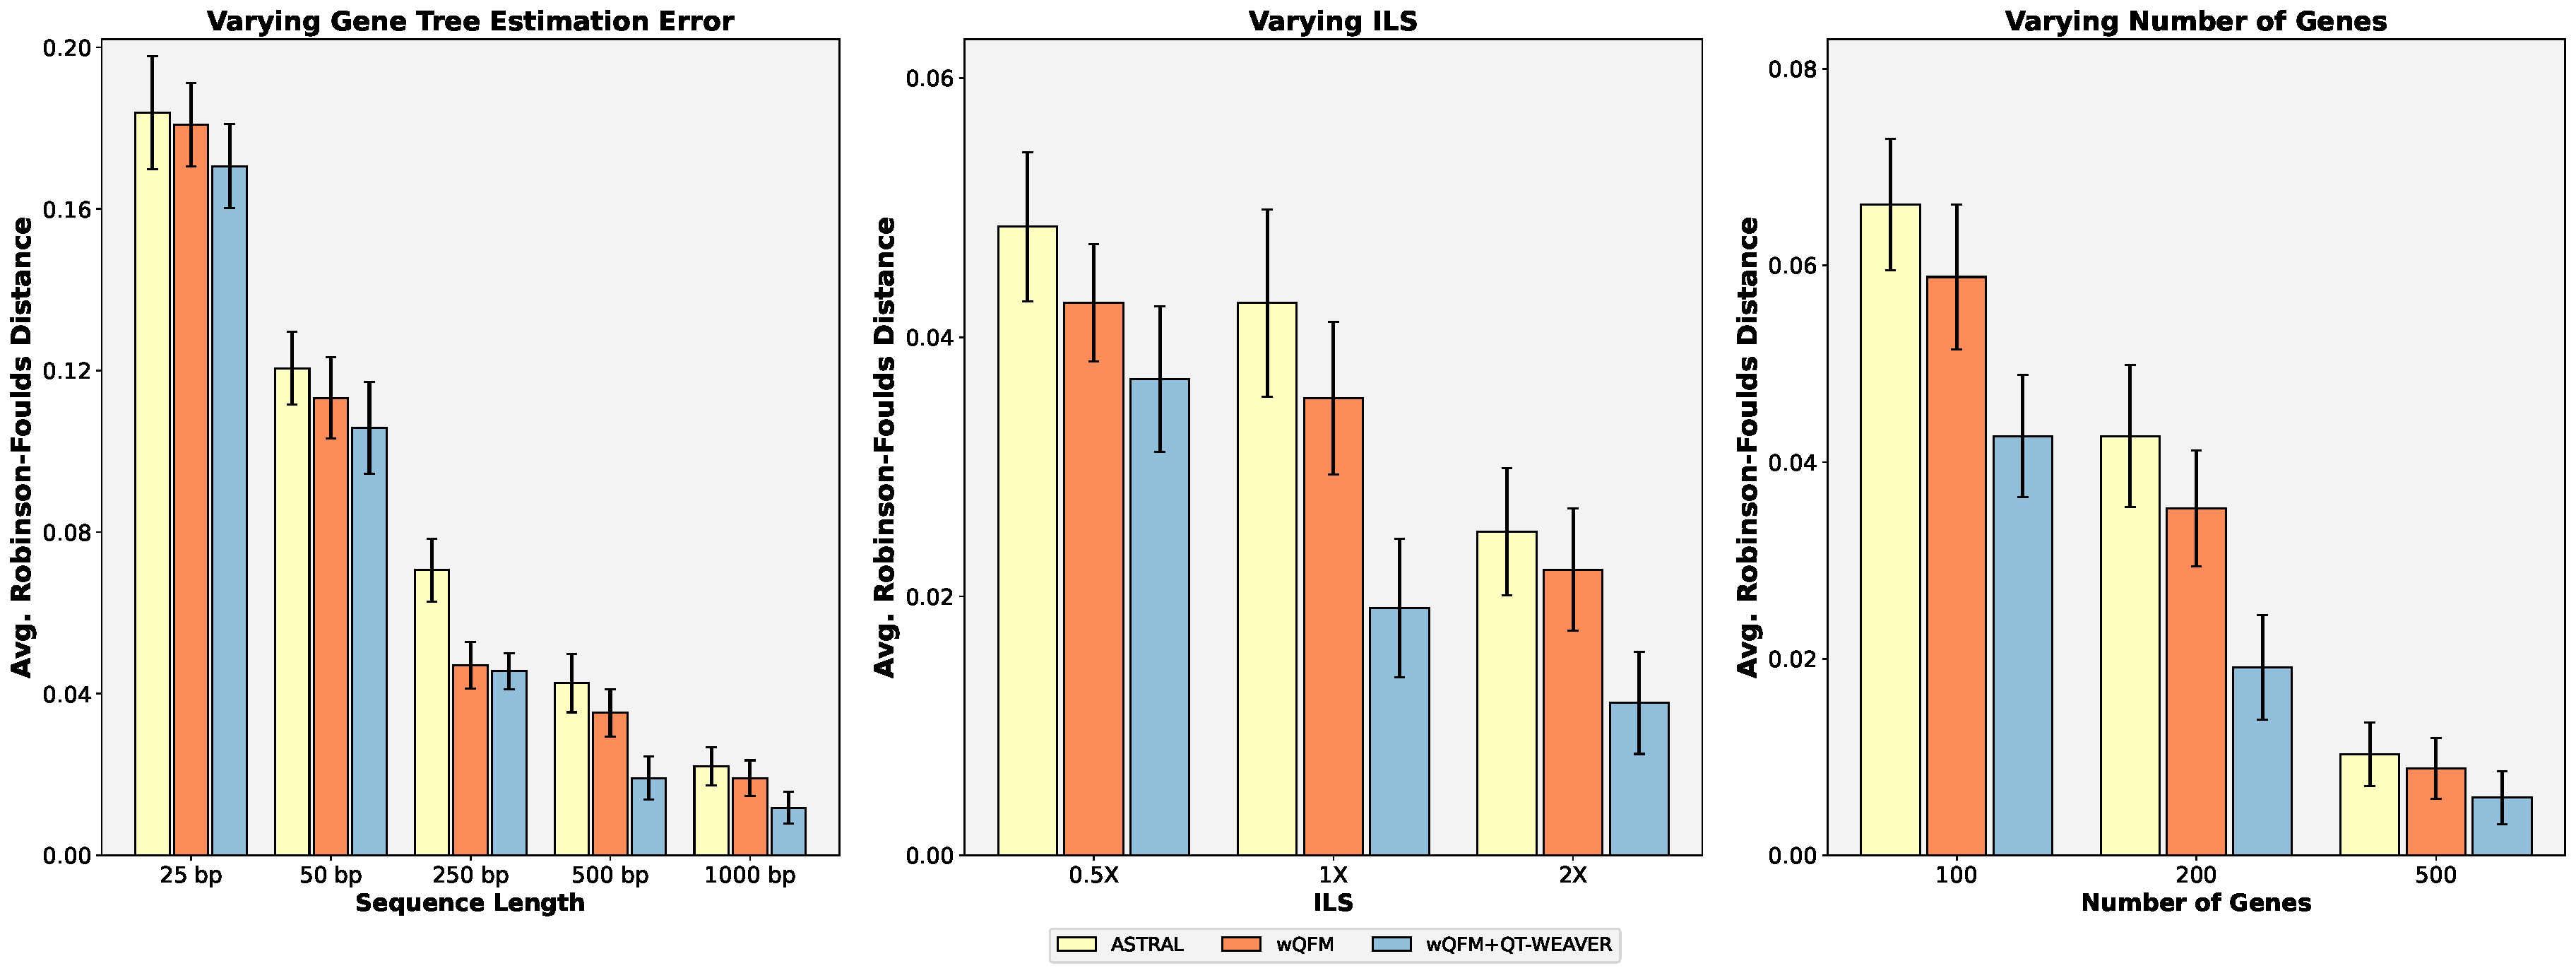
\includegraphics[width=\linewidth]{figures_new/2_37_methods.pdf}
    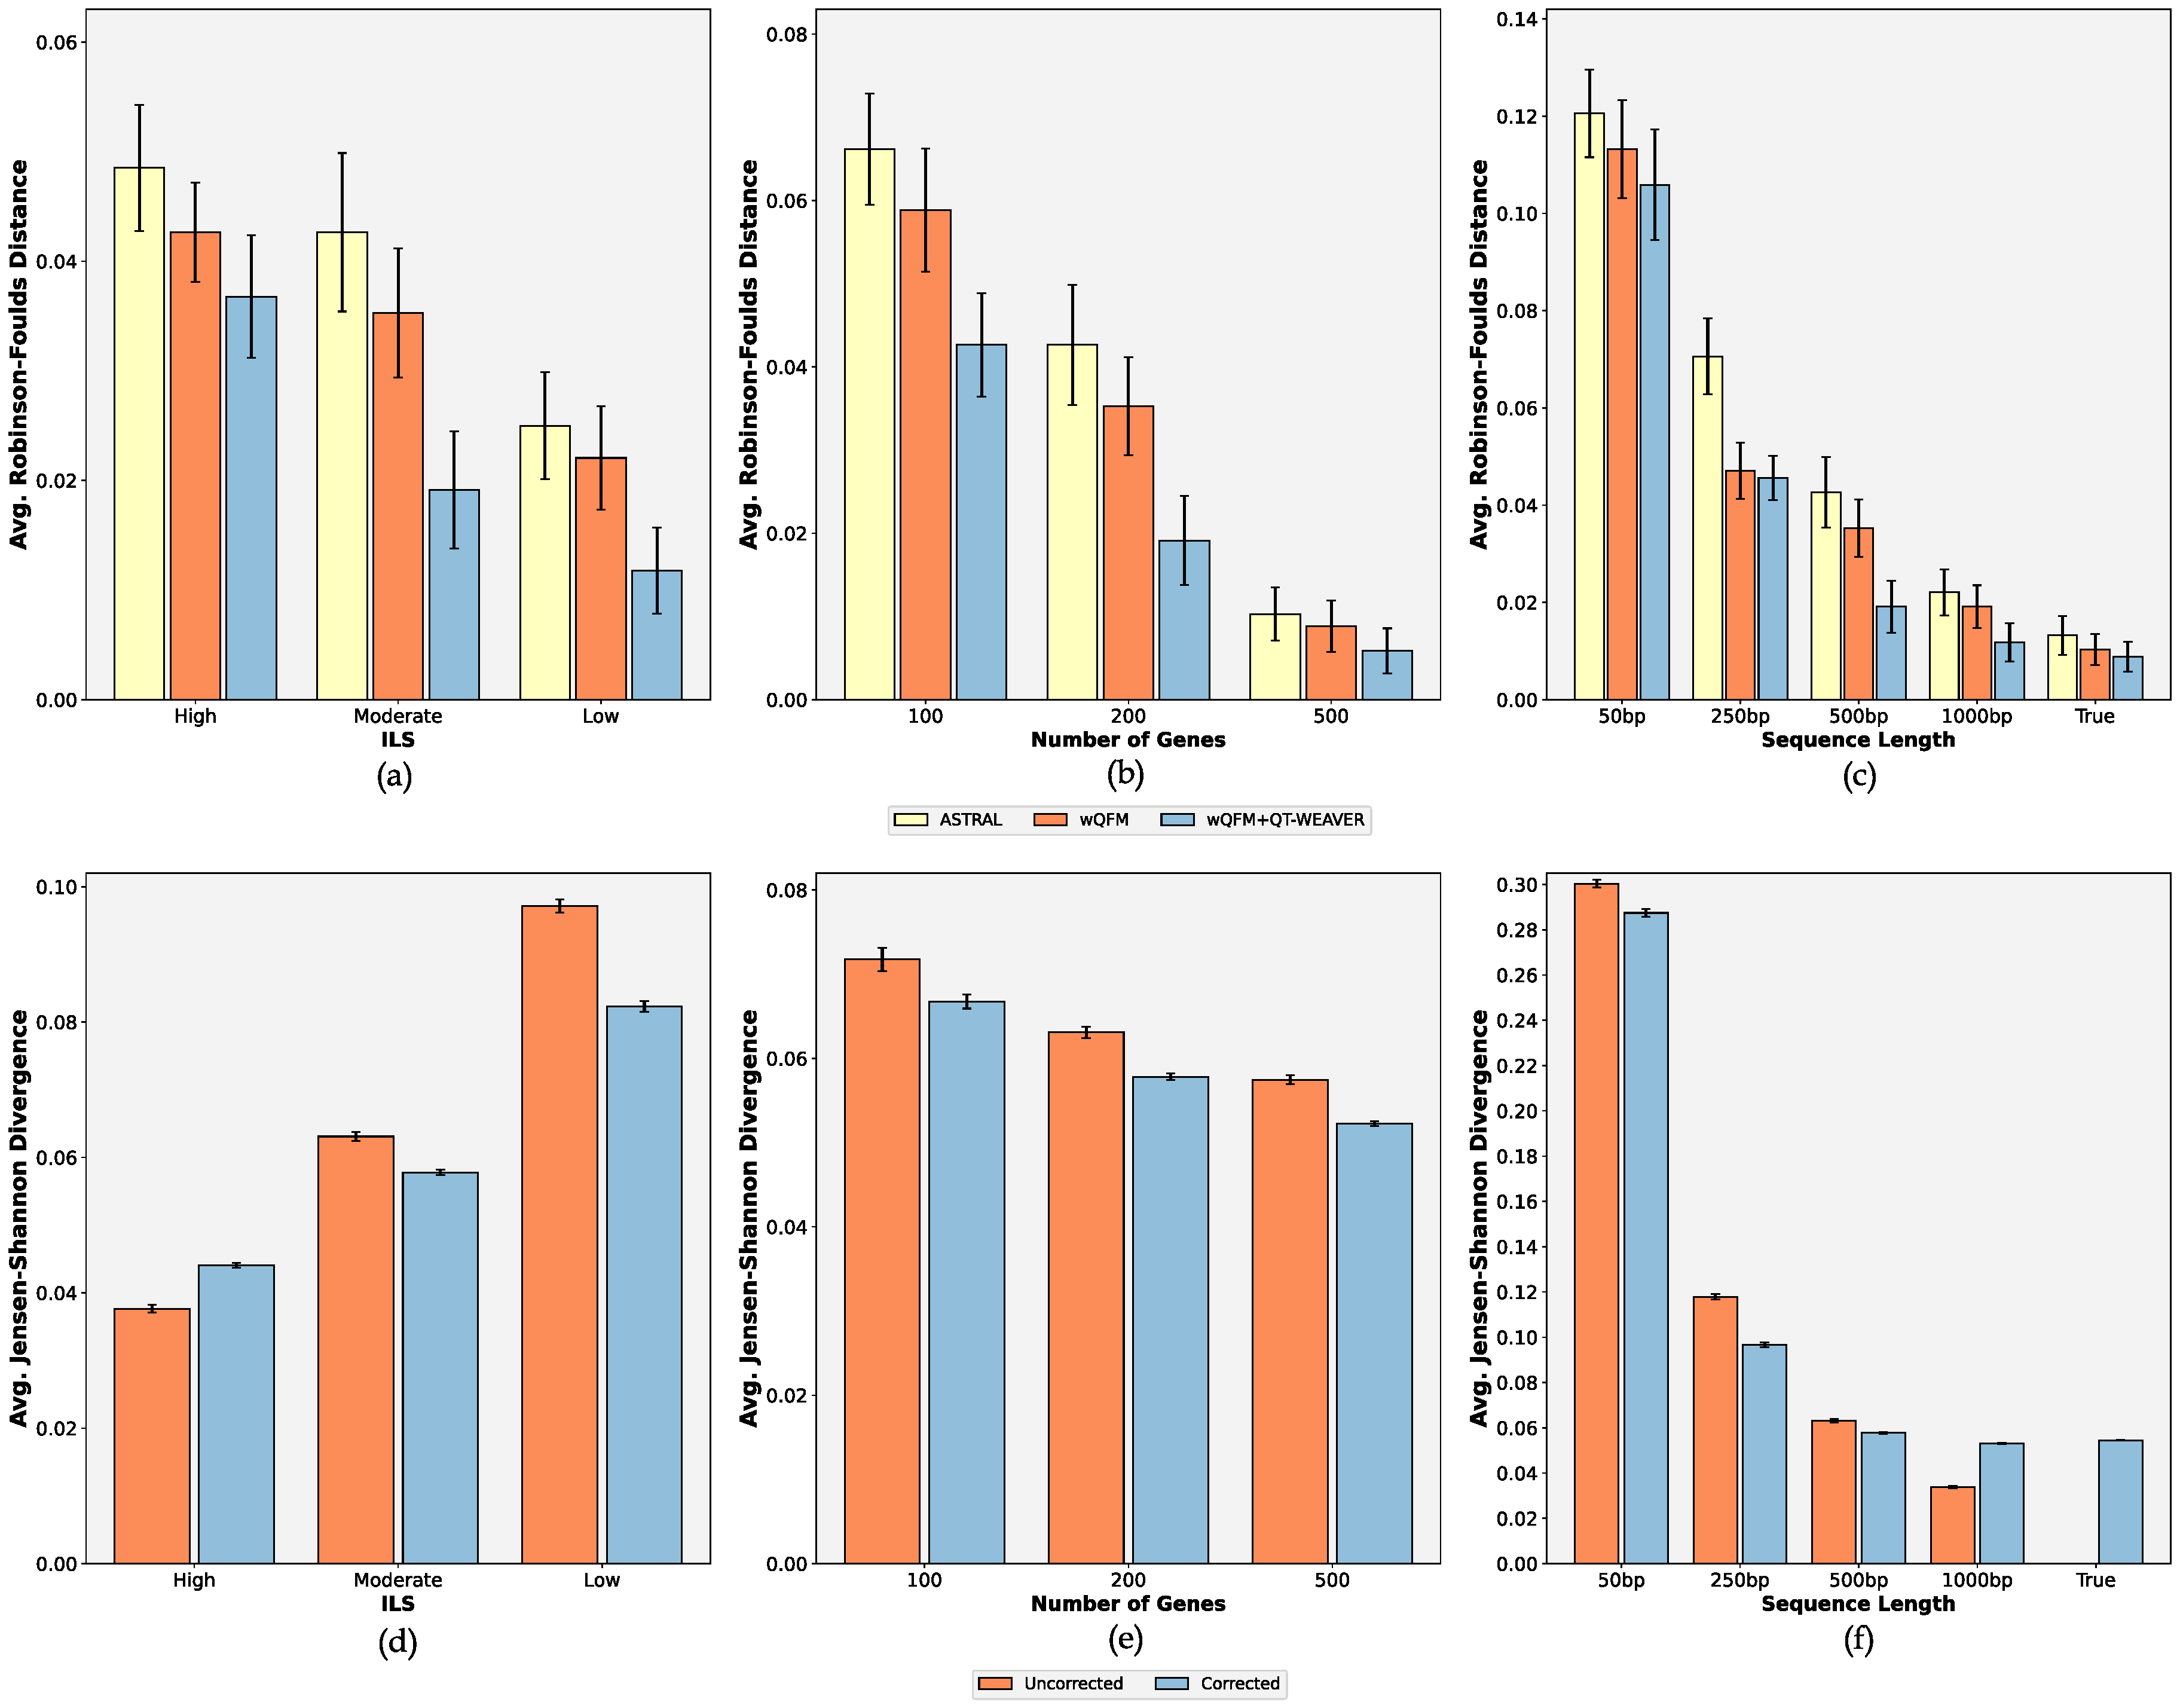
\includegraphics[width=0.75\linewidth]{figures_new/37-combined.pdf}
    \caption{\textbf{Results on 37-taxon dataset.} (a)-(c) We show the average RF rates with standard errors over 20 replicates for the methods ASTRAL, wQFM (wQFM-uncorrected), and wQFM+QT-WEAVER (wQFM-corrected). (a) The amount of ILS was varied from high to low, keeping the number of genes fixed at 200 and sequence length at 500bp. (b) The number of genes was varied keeping ILS fixed at moderate (1X) and the sequence length at 500bp. (c) Varying sequence lengths with moderate ILS and 200 genes. We also include true gene trees with no GTEE. (d)-(f) Average Jensen-Shannon divergence of the quartet distributions before and after correction with respect to the true quartet distributions. %The settings are identical to (a)-(c). 
    }
    \label{fig:rf_37_taxon_methods}
    \vspace{-10pt}
\end{figure}

% The following para is going to be Shorten due to space constraints. For journal version, we can use it.

%Both ASTRAL and wQFM estimate species trees by maximizing quartet scores, with ASTRAL offering the theoretical guarantee of identifying the species tree that maximizes quartet support within the search space defined by the bipartitions of the input gene trees. ASTRAL has been evolved and improved over successive versions for both accuracy and scalability, leaving limited (or no) scope for further enhancements in quartet score optimization. Thus, addressing gene tree estimation error (GTEE) becomes a critical avenue for pushing the accuracy frontier of quartet-based methods. In this context, the statistically significant improvements achieved by wQFM+QT-WEAVER across all model conditions in the 37-taxon dataset are particularly noteworthy.

ASTRAL has been evolved and improved over successive versions for both accuracy and scalability, offering the theoretical guarantee of identifying the species tree that maximizes quartet support within the search space defined by the bipartitions of the input gene trees and thereby leaving limited (or no) scope for further enhancements in quartet score optimization. Thus, addressing GTEE becomes a critical avenue for pushing the accuracy frontier of quartet-based methods. In this context, the substantial improvements achieved by wQFM+QT-WEAVER over ASTRAL %across all model conditions in the 37-taxon dataset are particularly 
is particularly noteworthy.

Next, we performed a series of experiments to further investigate the impact and quality of the quartet distributions produced by QT-WEAVER. First, to assess the similarity between the estimated quartet distributions (before and after correction) and the true quartet distributions (inferred from the true gene trees), we compare the Jensen-Shannon divergence between estimated and true quartet distributions in Figure \ref{fig:rf_37_taxon_methods}(d)-(f) and Table \ref{tab:37-divergence} in Appendix~\ref{app:37-taxon}. The corrected quartet distributions almost always have lower divergence than the uncorrected distributions, except for model conditions with very low divergence to begin with (less than 4 percent; 0.5x-200gt-500bp and 1X-200gt-1000bp conditions). The model conditions with relatively long sequence length (1000bp) have low amounts of GTEE and have less divergence to begin with (less than 4 percent), and correcting it does not seem to further reduce the divergence (rather making the distribution slightly more diverged). However, the corrected distributions overall result in better species trees as reflected by the RF rates (Figure \ref{fig:rf_37_taxon_methods}(c)). %as wQFM+QT-WEAVER produces better species trees than wQFM on the 1000bp model condition (Figure \ref{fig:rf_37_taxon_methods}(c)).
%Interestingly, the high ILS model condition (0.5X) has lower divergence compared to the low ILS model condition. However, the high levels of gene tree discordance in the high ILS dataset make species tree estimation challenging (reflected by RF rates).
Overall, these results suggest that QT-WEAVER effectively bridges the gap with the overall nature of the true distribution. %, resulting in more accurate trees estimated by wQFM+QT-WEAVER than ASTRAL and wQFM. %As an effect, wQFM+QT-WEAVER is able to estimate significantly more accurate species trees (Figure \ref{fig:rf_37_taxon_methods}).



%we measured the divergence between the weighted quartet distribution induced by true gene trees and the weighted quartet distributions of estimated gene trees using Jensen-Shannon divergence~\cite{jensen-shannon}. Jensen-Shannon divergence of original (uncorrected) and corrected (by QT-WEAVER) quartet distributions from true quartet distributions are shown in Figure~\ref{fig:rf_37_taxon_methods}(b). As we can see, the quartet distribution corrected by QT-WEVER is less diverged from the true distribution than the original (uncorrected) quartet distribution in all but two model conditions (0.5x-200gt-500bp and 1X-200gt-1000bp). These results show the efficacy of QT-WEVER in correcting the quartet distribution and supports the RF scores presented in Figure~\ref{fig:rf_37_taxon_methods}(a). \addb{we may want to explain why we see oppostie trends in 1000 bp condition even if the RF rate was improved}.

Next, we computed the quartet scores of different estimated species trees and the true species tree with respect to both estimated and true gene trees (see Tables \ref{tab:37-quartet-scores-estimated} and \ref{tab:37-quartet-scores-true}). When the quartet scores are computed based on original (uncorrected) estimated quartet distribution (Table \ref{tab:37-quartet-scores-estimated}), even though ASTRAL-estimated trees are less accurate than wQFM and wQFM+QT-WEAVER, ASTRAL achieves higher quartet scores than wQFM since ASTRAL is guaranteed to maximize the quartet score within a constrained search space. However, it ``overshoots'' the quartet score as it returns trees with higher quartet scores than the quartet score of the true tree. %Thus, maximizing the quartet scores with respect to the estimated gene trees may not guarantee more accuracy in the presence of gene tree estimation errors and limited number of genes, as the statistical consistency of quartet score maximization criterion holds when a sufficiently large number of true gene trees (without estimation error) is available. 
This is mostly because the statistical consistency of quartet score maximization criterion may not hold in the presence of gene tree estimation errors and limited number of genes.
The true tree having the lower quartet scores across all model conditions supports this claim (see also~\cite{spterrace,farah2020phylogenomic,hasan2024leveraging} for more related discussions). %This is mostly due to the presence of GTEE and limited numbers of genes as the statistical consistency of estimating species trees by maximizing the quartet score criterion holds when a sufficiently large number of true gene trees (without estimation error) is available.
The quartet scores of wQFM, especially wQFM+QT-WEAVER, with respect to the uncorrected estimated gene trees, are closer to the true quartet score than the scores of ASTRAL-estimated trees are to the true score. These further explain the superior performance of wQFM+QT-WEAVER over wQFM and ASTRAL. We also report the quartet score of wQFM+QT-WEAVER with respect to the quartet distribution corrected by QT-WEAVER. Notably, wQFM+QT-WEAVER has the highest quartet score when the score is computed based on the corrected quartet distribution. We note that these scores are not directly comparable to other methods' quartet scores as other reported scores are computed with respect to a different quartet distribution (i.e., original uncorrected distribution). Therefore, we cannot consider these scores as ``over-estimation'' compared to true quartet scores. Rather, it suggests that the weight adjustment/correction by QT-WEAVER results in quartet distributions that may lead to species trees with higher quartet consistency scores (w.r.t. corrected distributions), which were not attainable with the uncorrected distributions.

Finally, we examined the quartet scores with respect to true gene trees with no estimation errors (Table \ref{tab:37-quartet-scores-true}). The superiority of wQFM as a quartet-based tree estimation method and the efficacy of QT-WEAVER as a quartet correction method are even more evident from these quartet scores. %when they are computed with respect to the true gene trees (i.e., no estimation error). 
In most cases, wQFM and wQFM+QT-WEAVER achieve higher and closer (to true quartet score) quartet scores than ASTRAL. This implies that the corrected distributions result in species trees that better correspond to the true gene tree distribution -- supporting the trends observed in RF rates (Figure~\ref{fig:rf_37_taxon_methods}(a)). 

%ASTRAL estimates species trees by maximizing quartet scores, an approach that has been proven to be statistically consistent. It has gone through several iterations of refinement improving its performance even further. As a result, in terms of optimizing the quartet score, there is not much to be done beyond ASTRAL.

%We now analyze the results on the 37-taxon dataset in Figure \ref{fig:rf_37_taxon_methods}. To observe the impact of QT-WEAVER under different circumstances, we vary the gene tree estimation error (by varying the sequence length from 25 to 1000 bp), the amount of ILS (from low to high), and the number of genes (from 100 to 500). In every model condition, wQFM-corrected beats both ASTRAL and wQFM.

%In Figure \ref{fig:rf_37_taxon_methods}a, even though wQFM outperforms ASTRAL on all occasions, the improvements are not statistically significant (except for 250 bp). Conversely, after correction using QT-WEAVER, the improvements are statistically significant, barring the two most difficult model conditions (25 and 50 bp). In terms of varying ILS, the improvements are always significant compared to ASTRAL, which is never the case for wQFM (Fig. \ref{fig:rf_37_taxon_methods}b). Moreover, apart from the high ILS condition (0.5X), the advantage of wQFM-corrected over wQFM is also statistically significant.



%When the number of genes is varied, wQFM-corrected again attains a significant advantage over both ASTRAL and wQFM, except for 500 genes, where all three methods perform exceptionally well (Fig. \ref{fig:rf_37_taxon_methods}c).

%Like the 15-taxon dataset, we also assess the similarity with the true quartet distribution in Table \ref{tab:37-dom-mismatch-divergence} by comaparing the Jensen-Shanno divergence with the true distribution before and after correction. The corrected quartet distributions almost always have lower Jensen-Shannon divergence, except for model conditions with very low divergence to begin with (less than 4 percent). This suggests that QT-WEAVER effectively bridges the gap with the overall nature of the true distribution. As an effect, wQFM+QT-WEAVER is able to estimate significantly more accurate species trees (Fig. \ref{fig:rf_37_taxon_methods}).

% To further assess the similarity between the methods estimated quartet distributions (before and after correction) and the true quartet distributions, we also compare the Jensen-Shannon divergence in Table \ref{tab:15-divergence}. In this case, if the divergence is higher than 0.05, the corrected methods tend to close the gap with the true distribution. On the other hand, when the distribution has very low divergence to begin with, correcting it does not seem to reduce the difference. 

% \begin{table}[h!]
%     \centering
%     \small
%     % \tiny
%     \caption{Jensen-Shannon divergence with respect to the true gene trees for different model conditions averaged over all replicates. The best-performing method (i.e., lower divergence) for each model condition has been highlighted in bold. As the range of values varies across distributions, we normalize the sum of weights of the three topological variants of each quartet to 100 for both the estimated and true quartet distributions.}
%     % \bigskip
%     \label{tab:15-divergence}
%     \begin{tabularx}{1.1\textwidth}{|X|X|X|X|X|X|X|X|X|}
%     % {|c|c|c|c|c|c|c|c|c|}
%     \hline 
%         \textbf{Model Condition} & \textbf{GTF} & \textbf{GTF-corrected} & \textbf{GTF-BS} & \textbf{GTF-BS-corrected} & \textbf{GTF-MB} & \textbf{GTF-MB-corrected} & \textbf{SVD-Rec} & \textbf{SVD-Rec-corrected} \\
%         \hline
%         100gene-100bp & 0.115 & \textbf{0.103} & 0.133 & \textbf{0.121} & 0.114 & \textbf{0.101} & 0.147 & \textbf{0.138} \\
%         \hline
%         100gene-1000bp & \textbf{0.043} & 0.049 & 0.056 & \textbf{0.054} & \textbf{0.034} & 0.042 & 0.112 & \textbf{0.111} \\
%         \hline
%         1000gene-100bp & 0.101 & \textbf{0.087} & 0.123 & \textbf{0.111} & 0.104 & \textbf{0.089} & \textbf{0.1} & 0.107 \\
%         \hline
%         1000gene-1000bp & \textbf{0.031} & 0.037 & 0.05 & \textbf{0.047} & \textbf{0.025} & 0.033 & \textbf{0.131} & 0.175 \\
%         \hline
%     \end{tabularx}
% \end{table}

%We again assess the quartet scores like we did for the 15-taxon dataset in Tables \ref{tab:37-quartet-scores-estimated} and \ref{tab:37-quartet-scores-true}. For the estimated gene trees, ASTRAL once again obtains the highest scores while generating the least accurate species trees, suggesting that it suffers from ``overshooting". In most model conditions, wQFM+QT-WEAVER obtains the closes scores to the true tree. Once again, in terms of the corrected distribution, the quartet scores of wQFM+QT-WEAVER are by far the highest, indicating how maximizing the quartet scores with respect to the corrected distribution is less prone to ``overshooting".

%However, the results for the true gene trees are somewhat mixed on this occasion (Table \ref{tab:37-quartet-scores-true}). All three methods obtain the best quartet scores in a few model conditions. \addb{not sure how to explain}
% Even though wQFM+QT-WEAVER fails to always obtain the best quartet scores in terms of the true gene trees, it consistently outperforms the other methods; which suggests that 


% After assessing both tables, we can claim that if the original distribution is very close to the true distribution, correcting it may increase the gap slightly. Despite that, the corrected distributions are able to better capture the true species tree (Fig. \ref{fig:rf_15_taxon_methods}).

% As it is clear that our correction procedure on the original distribution clearly improves its performance, it begs the question: what if we correct the new distribution again? To address this, we perform 50 iterations of correction and analyze how different metrics evolve in Figure \ref{fig:rf_15_taxon_iterative}. On model conditions with high gene tree estimation errors, the rf rates improve steadily (Fig. \ref{fig:rf_15_taxon_iterative}a). On the other hand, in model conditions where the rf rate is low from the earlier iterations (less
% than 5 percent), the results deteriorate with subsequent iterations. Even on the 1000gene-100bp model condition, where the rf rate improves drastically from 15 percent to below 5 percent after around 15 iterations, the result worsens with further iterations. The shapes of the dominant quartet's mismatch curves closely resemble the rf curves, signifying a high correlation between the two (Fig. \ref{fig:rf_15_taxon_iterative}b).

% \begin{figure}[h]
%     \centering % <-- added
%     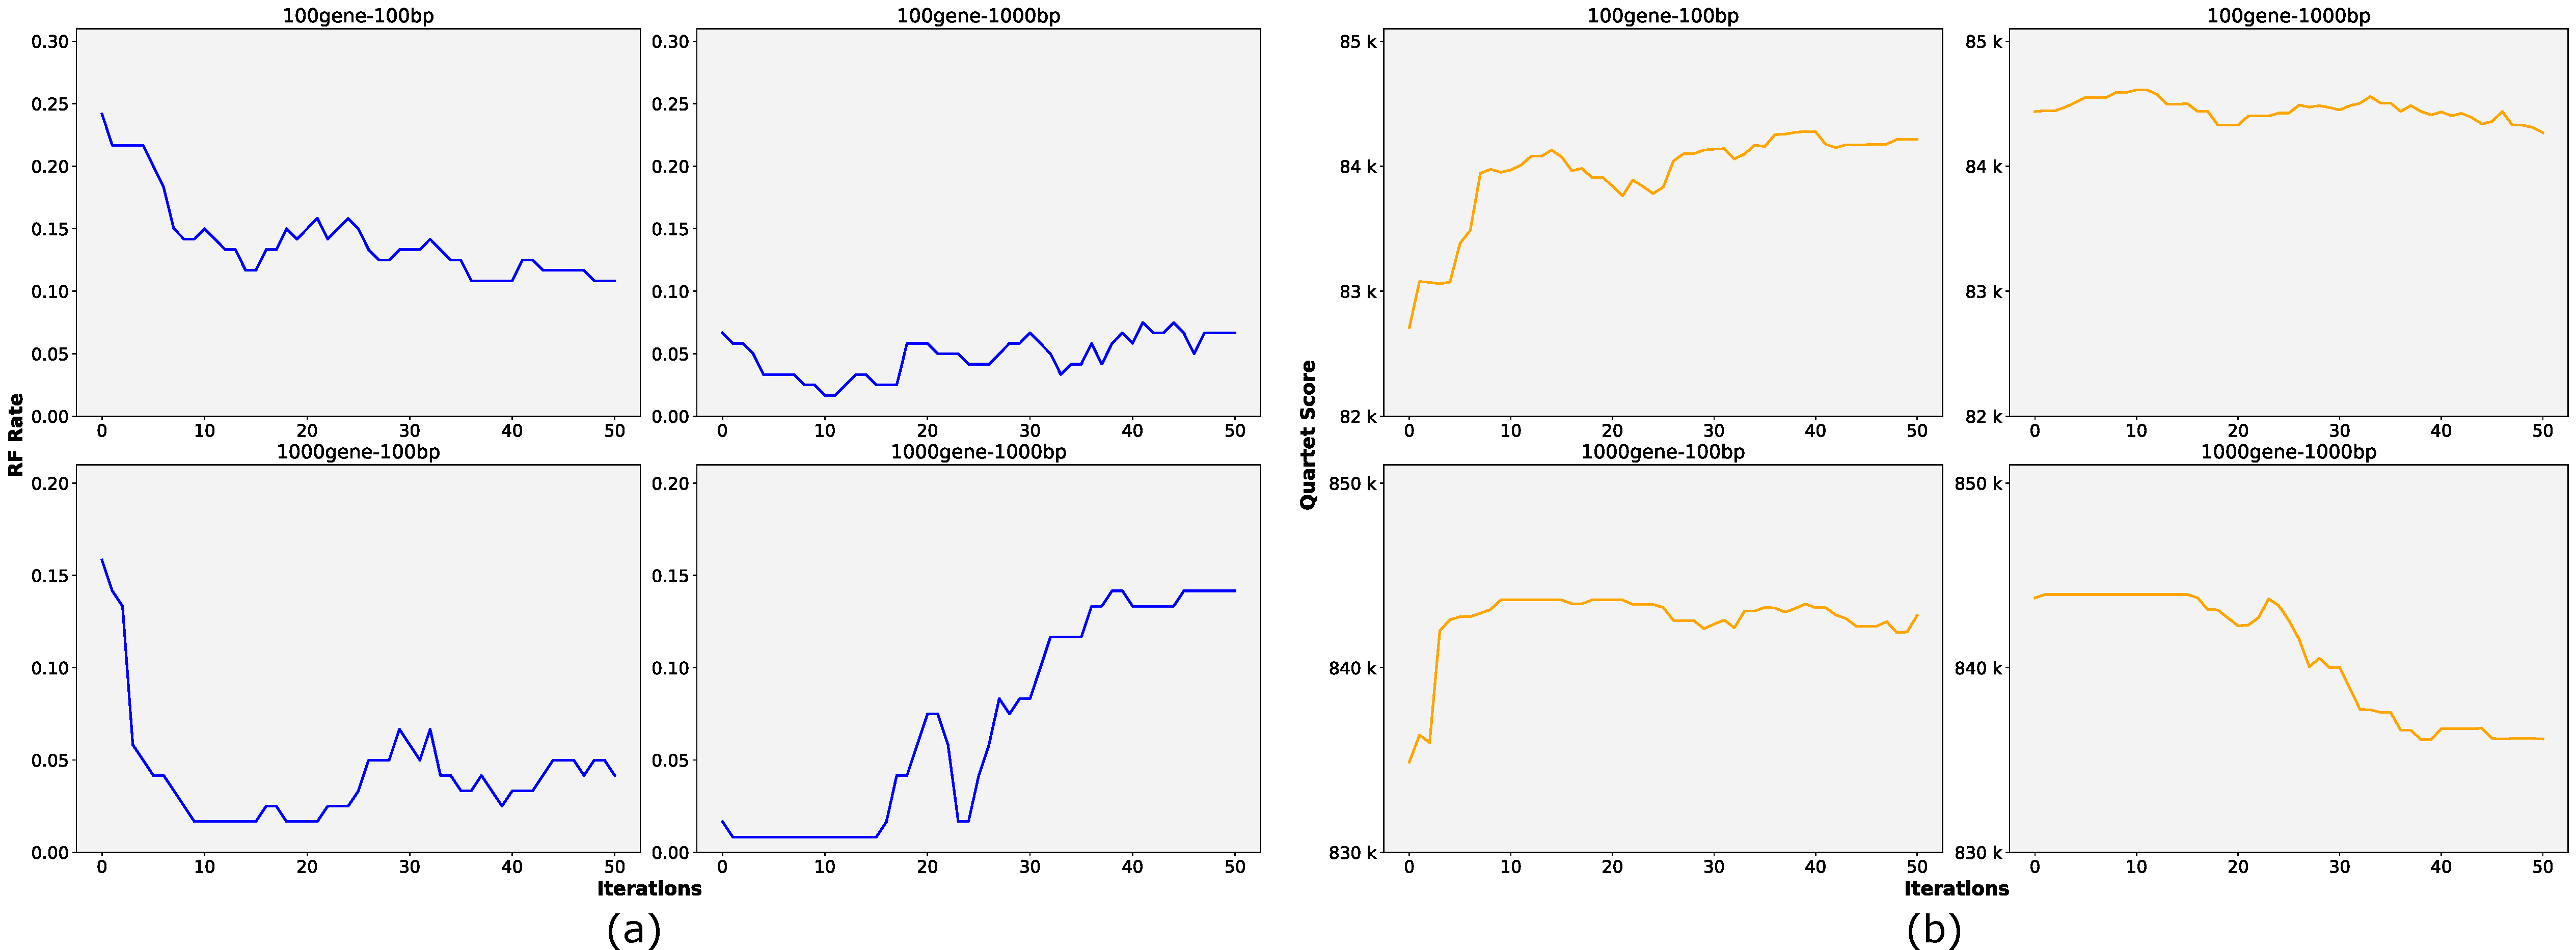
\includegraphics[width=\linewidth]{figures_new/15_iterative.pdf}
%     \caption{\textbf{Results on 15-taxon dataset.} We show the changes in four different metrics after running 50 iterations of correction. The input of each iteration was the output of the last. The four metrics are: (a) RF rates, (b) Number of mismatched dominant quartets w.r.t to the true gene trees, (c) Quartet score of the estimated species tree with respect to its corresponding quartet distribution, and (d) Jensen-Shannon divergence w.r.t the true quartet distribution.}
%     \label{fig:rf_15_taxon_iterative}
% \end{figure}

% On the other hand, the divergence curves all follow the same rising pattern (Fig. \ref{fig:rf_15_taxon_iterative}d). Even for instances where rf rate is quite low, the divergence can be quite high. This is because, in the true distribution, a few gene trees support the wrong quartet topologies due to ILS. But the corrected distributions keep decreasing the weights of these incorrect topologies over iterations, eventually (and hopefully)( making them zero. Thus, despite the high divergence, the estimated species trees are remarkably accurate. In Figure \ref{fig:rf_15_taxon_iterative}c, we observe that the quartet scores of the estimated species trees rise gradually in relation to their corresponding distributions, reaching nearly 100 percent score. Upon close inspection of the rf curves and the quartet score curves, trees with quartet scores of around 90-93 tend to attain decent rf rates across all model conditions. Thus, the quartet score of 90 could be a viable stopping criterion for the iterations.

\subsection{Results on 15-taxon dataset}

In the simulated 15-taxon datasets, we evaluated the performance on varying gene tree estimation errors using 100bp and 1000bp sequence lengths and on varying numbers of gene trees (100 and 1000). Similar to the 37-taxon dataset, wQFM+QT-WEAVER consistently outperforms ASTRAL and wQFM across all four model conditions (Figure \ref{fig:rf_15_taxon_methods}). In particular, wQFM+QT-WEAVER is significantly better ($p \ll 0.05$) than ASTRAL on challenging model conditions with short sequences (100bp), i.e., high GTEE. %amounts of gene tree estimation error. %As expected, all methods showed lower error rates with increasing sequence lengths and increasing numbers of genes. 

Similar to 37-taxon dataset, we investigated the divergence of uncorrected and corrected quartet distributions from true quartet distributions (Figure~\ref{fig:rf_15_taxon_methods}(c)-(d) and Table \ref{tab:15-divergence}) and the quartet scores of different estimated species trees with respect to both estimated and true gene trees (see Appendix~\ref{app:15-taxon}). 
The Jensen-Shannon divergence clearly improves after correction when the gene tree estimation error is high (100bp). Thus, the quartet distributions inferred from gene trees with high estimation error realign with the true distribution after correction using QT-WEAVER. On the other hand, when the distribution has low amounts of GTEE with relatively long (1000bp) sequences and thus very low divergence to begin with ($\le 5$\%), correcting it does not seem to reduce the difference. Interestingly, even though the divergence increases slightly for the more accurate distributions (1000bp), the corrected distribution as a whole seems to be more representative of the true distribution, as supported by the better RF rates.

We again assess the quartet scores like we did for the 37-taxon dataset in Tables \ref{tab:15-quartet-scores-estimated} and \ref{tab:15-quartet-scores-true}, and observed similar trends. wQFM+QT-WEAVER achieves higher and closer (to true quartet score) quartet scores than ASTRAL and wQFM across all four model conditions when the quartet scores are computed based on true gene trees -- further demonstrating the efficacy of QT-WEAVER in accounting for GTEE. %These results support our claim that QT-WEAVER effectively accounts for gene tree estimation error while imputing the missing quartets.


%\add{We now compare the effectiveness of wQFM + QT-WEAVER on different types of model conditions with wQFM (on original distribution) and ASTRAL, two of the most prominent quartet-based coalescent methods in Figure \ref{fig:rf_15_taxon_methods}. ASTRAL estimates species trees by maximizing quartet scores, an approach that has been proven to be statistically consistent. It has gone through several iterations of refinement improving its performance even further. As a result, in terms of optimizing the quartet score, there is not much to be done beyond ASTRAL. Therefore, we chose to shift our focus to a different direction: ``correcting" the quartet distribution based on conflicting sets.}

\begin{figure}[h!]
    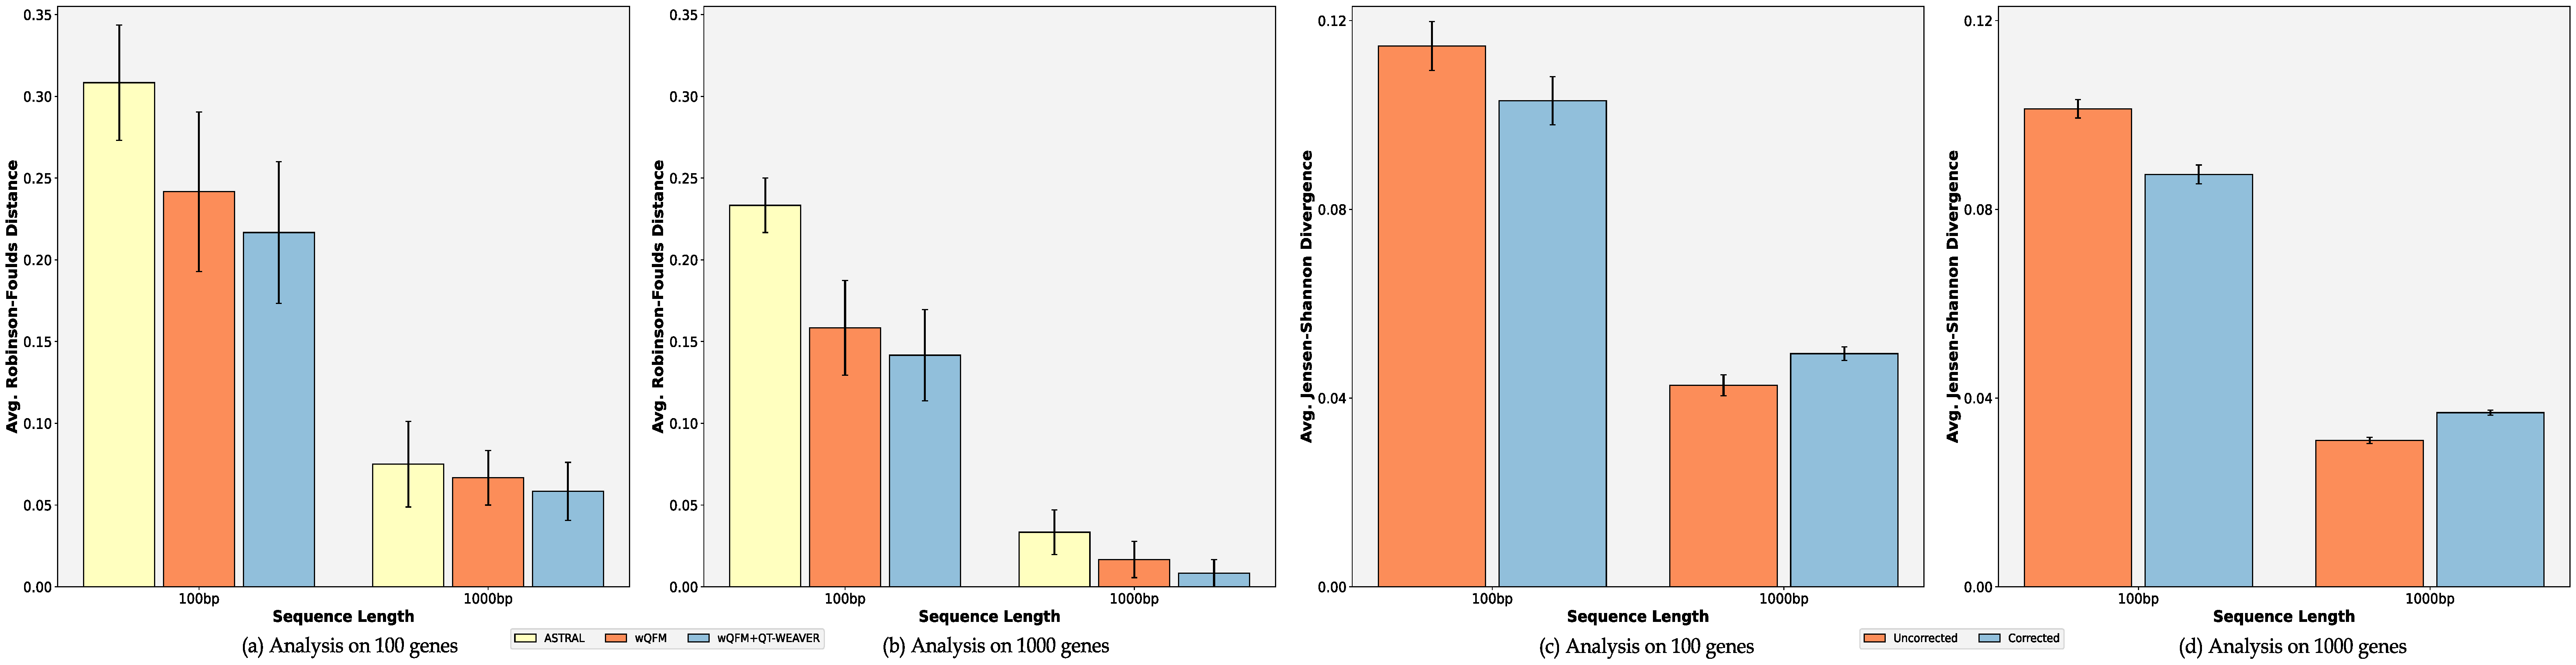
\includegraphics[width=\linewidth, height=0.3\linewidth]{figures_new/15-combined.pdf}
    \caption{\textbf{Results on 15-taxon dataset.} (a)-(b) Average RF rates of ASTRAL, wQFM, and wQFM+QT-WEAVER on varying model conditions with varying sequence lengths and numbers of genes. %We vary the gene tree estimation error by alternating the number of base pairs per gene sequence between 100 and 1000. The results have been reported on model conditions with (a) 100 genes and (b) 1000 genes. 
    (c)-(d) Average Jensen-Shannon divergence for the uncorrected and corrected quartet distributions.}
    \label{fig:rf_15_taxon_methods}
\end{figure}

%It is easy to see that the output distributions of QT-WEAVER result in more accurate trees across all model conditions (Fig. \ref{fig:rf_15_taxon_methods}). It consistently outperforms ASTRAL; the improvement being statistically significant in all but the 100gene-1000bp model condition.

%One of the secondary goals of the correction heuristic is to steer the estimated quartet distribution closer to the true distribution. 
% To assess this, we compare the number of dominant quartets in the estimated distribution that differ from the dominant quartets in the true gene trees before and after correction in Table \ref{tab:15-dom-mismatch-divergence}. 
%To assess the similarity between the estimated quartet distributions (before and after correction) and the true quartet distributions (inferred from the true gene trees), we compare the Jensen-Shannon divergence between the two in Table \ref{tab:15-dom-mismatch-divergence}. A very interesting pattern is observed. The Jensen-Shannon divergence clearly improves after correction when the gene tree estimation error is high (100bp). On the other hand, when the distribution has very low divergence to begin with (less than 5 percent), correcting it does not seem to reduce the difference.

%Thus, we can deduce that quartet distributions inferred from gene trees with high estimation error realign with the true distribution after correction. Interestingly, even though the divergence increases slightly for the more accurate distrib utions, the corrected distribution as a whole seems to be more representative of the true distribution, as backed up by the better RF rates.

%We now assess the quartet scores of the species trees estimated by different methods with respect to the sets of estimated gene trees as well as the true gene trees (Table \ref{tab:15-quartet-scores-estimated} and \ref{tab:15-quartet-scores-true}). In terms of true gene trees, the true tree has the highest quartet scores as expected due to that statistical consistency of quartets. Secondly, the best proven method, wQFM+QT-WEAVER yields the highest quartet scores, followed by wQFM and ASTRAL respectively. This implies that the corrected distributions result in species trees which better correspond to the true gene tree distribution. The lower RF rates of wQMF+QT-WEAVER further enforce that methods that optimize the quartet score with respect to the true gene trees obtain the most accurate results.

\vspace{-22pt}
\section{Iterative corrections using QT-WEAVER}

%Our results on the 37- and 15-taxon datasets clearly demonstrate 
The demonstrated effectiveness of using QT-WEAVER in adjusting quartet distribution begs the question: what happens if we iteratively correct the adjusted distribution, using the output of QT-WEAVER as input to QT-WEAVER for the next iteration? To investigate this, we performed 50 iterations on 15-taxon dataset and analyzed how different evaluation metrics evolve in Figure \ref{fig:rf_15_taxon_iterative}. Notably, in model conditions with high gene tree estimation errors (100bp), RF rates steadily and dramatically improve (Figure \ref{fig:rf_15_taxon_iterative}a). For the 100bp-100gene condition, the RF rate drops from 25\% to 11\% after 15 iterations of weight corrections, and for the 100bp-1000gene condition, the RF rate decreases from 16\% to as low as 2\% after 10 iterations. Note that the RF rates of ASTRAL on these two model conditions are 31\% and 23\%, respectively, as indicated by the horizontal lines in Figure \ref{fig:rf_15_taxon_iterative}a. However, in model conditions with well-estimated gene trees (1000bp sequences) where the initial RF rates are already low ($\sim 5\%$), repeated iterations may initially improve accuracy (e.g., a drop from 7\% to 1\% in the 1000bp-100gene condition) but eventually lead to performance degradation. This occurs because continuously adjusting well-estimated and corrected quartet distributions (as in cases with long sequences and large numbers of genes) can distort the weights to an extent that can mislead the tree search algorithm toward less accurate trees.

%Even on the 1000gene-100bp model condition, where the rf rate improves drastically from 15 percent to below 5 percent after around 15 iterations, the result worsens with further iterations. The shapes of the dominant quartet's mismatch curves closely resemble the rf curves, signifying a high correlation between the two (Fig. \ref{fig:rf_15_taxon_iterative}b).

\begin{figure}[htbp]
    \centering % <-- added
    % 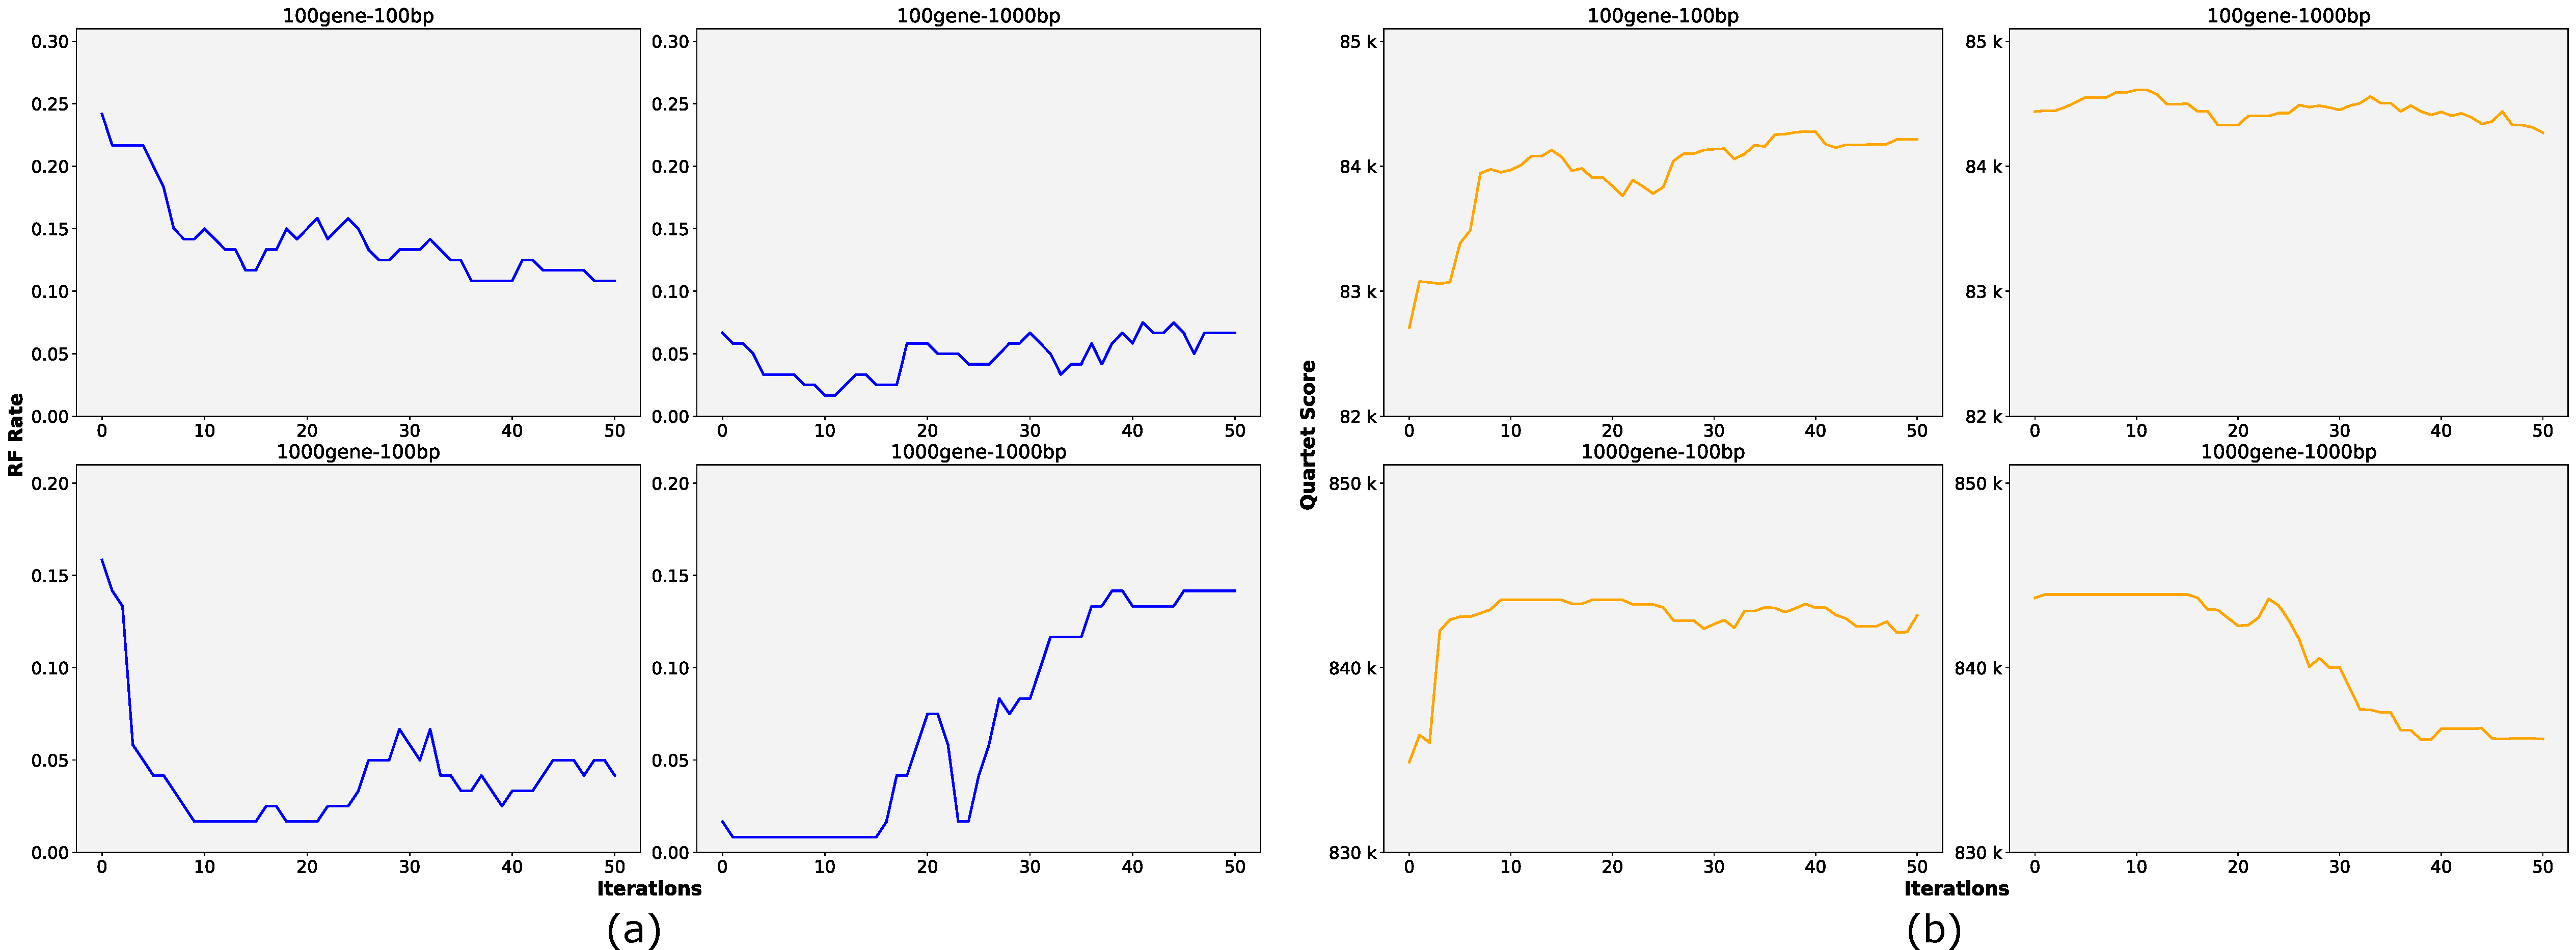
\includegraphics[width=\linewidth, height=0.45\linewidth]{figures_new/15_iterative.pdf}
    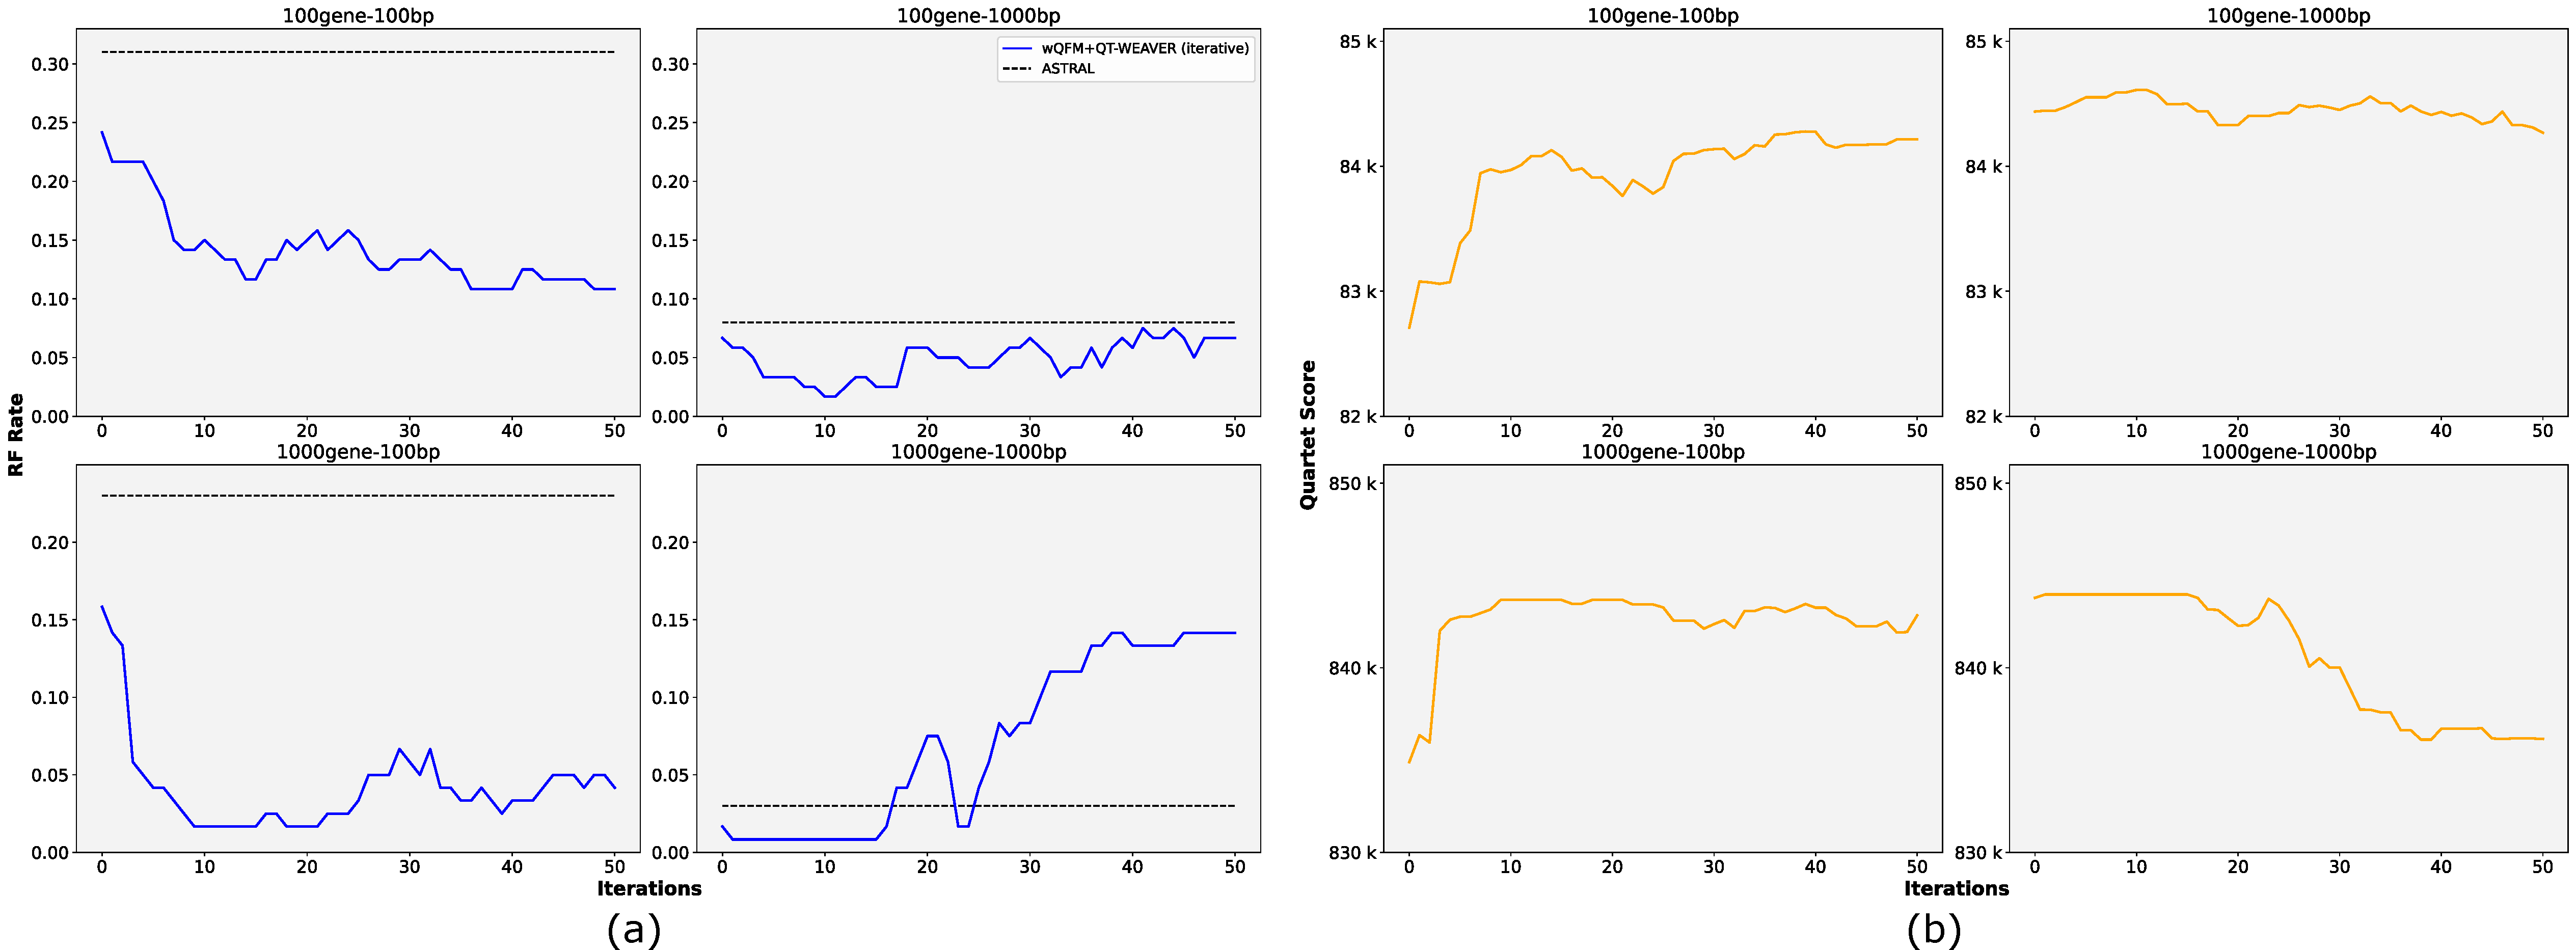
\includegraphics[width=\linewidth, height=0.4\linewidth]{figures_new/15_iterative_astral.pdf}
    \caption{\textbf{Iterative corrections on the 15-taxon dataset.} We show the changes in RF rates and quartet scores (with respect to true gene trees) of wQFM+QT-WEVER over 50 iterations of weight corrections using QT-WEAVER. ASTRAL's RF rates are indicated by dashed horizontal lines in (a).
    %The input of each iteration was the output of the last. The two metrics are: (a) Average RF distance, (b) Average quartet scores with respect to the true gene trees.
    % (c) Quartet score of the estimated species tree with respect to its corresponding quartet distribution, and (d) Jensen-Shannon divergence w.r.t the true quartet distribution.
    }
    \label{fig:rf_15_taxon_iterative}
    \vspace{-10pt}
\end{figure}



In Figure \ref{fig:rf_15_taxon_iterative}(b), we show the changes in quartet scores (w.r.t. the true gene tree distributions) for wQFM+QT-WEAVER over multiple iterations. As we can see, the increase and decrease in the quartet scores over multiple iterations are perfectly aligned with the decrease and increase of the RF rates, respectively. When the GTEE is high, the scores maintain a rising trend. On the other hand, on the low GTEE model conditions, the quartet scores start to degrade after a few iterations in a pattern identical to the RF rate degradation. Additionally, we investigated the Jensen-Shanon divergence and quartet scores (relative to corrected distributions) across iterations (Figure \ref{fig:rf_15_taxon_iterative_2} and related discussion in Appendix \ref{app:iterations}).

%Additionally, we investigated how the Jensen-Shanon divergence evolves across iterations (see Figure \ref{fig:rf_15_taxon_iterative_2}(a) in Appendix \ref{app:iterations}). Initially, the divergence decreases during the first one or two iterations but then begins to increase. This occurs because, for the three alternative quartet topologies ($ab|cd, ac|bd, ad|bc$) on four taxa, QT-WEAVER tends to prioritize the quartet topology it identifies as ``correct'' --the one with the least conflict score--by increasing its weight while reducing the weights of the alternative topologies.  Thus, with successive iterations, the weight of the ``correct'' quartet topology continues to rise (toward 100\%) while the weights of the other two alternatives keep decreasing (toward 0\%). Thus, this overestimation of the weight of the ``correct'' quartets and the underestimation of the weights of the ``incorrect'' ones lead the adjusted distribution to diverge from the true weighted distribution. Despite this divergence, the iterative adjustments may still guide the tree search algorithm toward more accurate trees (up to a certain point) by emphasizing and amalgamating the quartets with higher weights, as evidenced by the gradual decrease in the RF rates up to 10-15 iterations. For the same reason, when examining the quartet scores of wQFM+QT-WEAVER with respect to the corresponding corrected quartet distribution (instead of the original quartet distribution), the scores continue to increase, approaching nearly 100\% (see Figure \ref{fig:rf_15_taxon_iterative_2}(b) in Appendix \ref{app:iterations}). This occurs because, in the corrected distribution, the weights of the quartets present in the estimated species trees steadily rise, resulting in higher quartet scores for the estimated trees.


Thus, performing multiple iterations of weight adjustment shows potential, though improvements may not be consistent across all datasets. For instance, in the 37-taxon dataset, no further improvement was seen beyond the first iteration, as in most cases, the RF rates dropped below 5\% after one iteration, and successive iterations distorted the distributions to an extent that resulted in worse trees. Nonetheless, QT-WEAVER’s iterative approach shows promise and warrants further investigation to develop a robust stopping criterion and scoring scheme for selecting the best tree from successive iterations.
%Nevertheless, the iterative approach using QT-WEAVER holds promise and justifies further investigation to develop an effective stopping criterion and a scoring scheme to find and return the tree with the best score from successive iterations. 

%We hypothesize that selecting a suitable subset of 28 conflicting pair as a configuration setting of the QT-WEAVER algorithm (see Section~\ref{sec:configuration} based on the nature of the input gene trees may help improve the performance of QT-WEVAER


%On the other hand, the divergence curves all follow the same rising pattern (Fig. \ref{fig:rf_15_taxon_iterative}d). Even for instances where rf rate is quite low, the divergence can be quite high. This is because, in the true distribution, a few gene trees support the wrong quartet topologies due to ILS. But the corrected distributions keep decreasing the weights of these incorrect topologies over iterations, eventually (and hopefully)( making them zero. Thus, despite the high divergence, the estimated species trees are remarkably accurate. In Figure \ref{fig:rf_15_taxon_iterative}c, we observe that the quartet scores of the estimated species trees rise gradually in relation to their corresponding distributions, reaching nearly 100 percent score. Upon close inspection of the rf curves and the quartet score curves, trees with quartet scores of around 90-93 tend to attain decent rf rates across all model conditions. Thus, the quartet score of 90 could be a viable stopping criterion for the iterations.


\vspace{-10pt}
\section{Results on biological avian dataset}

%\paragraph{Avian dataset.}
We have reanalyzed the avian biological dataset from \cite{jarvis2014}, which has 14,446 genes (including exons, introns, and UCEs) across 48 taxa. This dataset contains high levels of gene tree discordance likely driven by rapid radiation events in the evolutionary history of these species. Mahbub et al. \cite{wqfm} compared ASTRAL, wQFM, and wQMC with the binned MP-EST tree which was presented in Jarvis \textit{et al.}~\cite{jarvis2014}. We include wQFM+QT-WEAVER in this comparison (Figure \ref{fig:avian} in Appendix~\ref{app:avian-biological}). %We used the ``PoW" weighting scheme for correction in this scenario as it generated a better tree than its counterpart.

%moved to appendix

% \begin{figure}[t!]  
% \centering
%     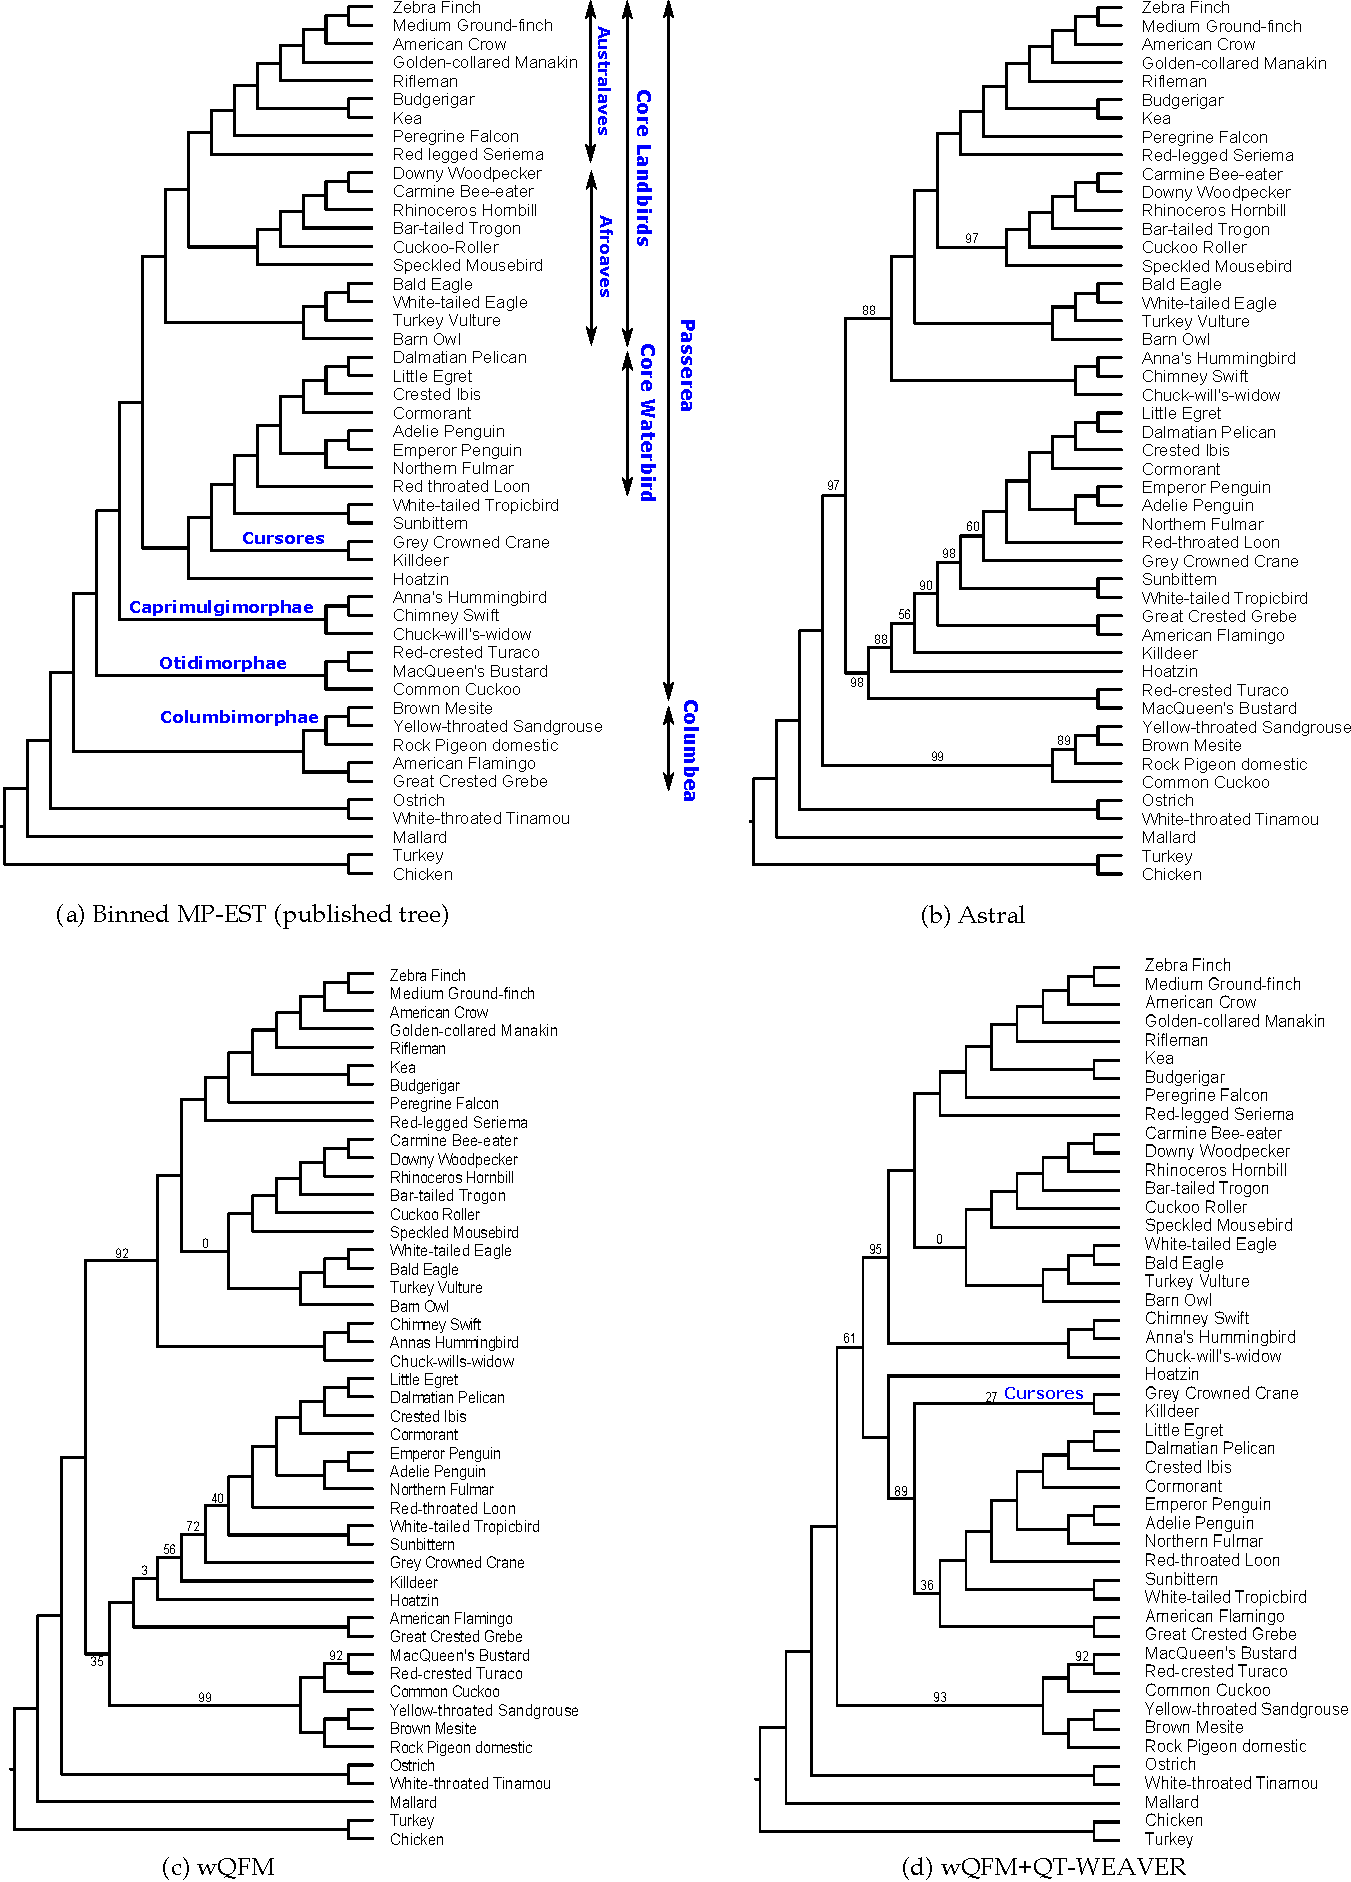
\includegraphics[width=0.85\linewidth]{figures_new/avian-combined-v2.pdf}
%     \caption{\textbf{Analyses of the avian dataset using ASTRAL and wQFM (before and after correction).} 
%     Branch supports are computed based on quartet-based local posterior probability~\cite{sayyari2016fast} (multiplied by 100). All BS values are 100\% except where noted.}
%     \label{fig:avian}
% \end{figure}

All three estimated trees are highly congruent with the reference binned tree, with wQFM+QT-WEAVER being the most congruent and ASTRAL the least. %Still, all three failed to reconstruct some well-established sub-groups by the avian phylogenomics project and other studies. 
The wQFM trees (on uncorrected and corrected distributions) are almost identical, with mainly one noticeable difference: wQFM+QT-WEAVER was able to correctly resolve the Cursores clade (crane and killdeer), which both wQFM and ASTRAL failed to recover. ASTRAL failed to recover Otidimorphae (bustard, turaco, and cuckoo), whereas both wQFM and wQFM+QT-WEAVER reconstructed this clade.

All three methods successfully reconstructed the well-established Australaves clade (passeriformes, parrots, falcons, and seriemas). They also recovered the Afroaves, Core Waterbird, and Caprimulgimorphae clades successfully.
ASTRAL failed to recover Otidimorphae, unlike both the wQFM methods.  All three failed to recover Columbea but were able to recover the constituent clades Columbimorphae (mesite, sandgrouse, and pigeon) and Phoenicopterimorphae (flamingo and grebe).

\vspace{-10pt}
\section{Running Time}
The running time of QT-WEAVER solely depends on the number of taxa $n$ and not on the number of genes, which determines the number of unique quartets ($3$$n \choose 4$) in the weighted quartet distribution.
All analyses were run on the same machine with AMD Ryzen 7 5800H CPU (8 cores), 16GB RAM, and NVIDIA GeForce RTX 3060 GPU (6GB memory). The simulated 15-taxon and 37-taxon datasets took 1.65 and 242 seconds on average per replicate. The biological avian dataset with 48 taxa took 983 seconds to run.

%As the number of quartets grows exponentially with the number of taxa, so does the runtime.

% \begin{table}[]
%     \centering
%     \caption{Caption}
%     \label{tab:runtimes}
%     \begin{tabular}{|c|c|c}
%         Dataset & Taxa & Runtime (seconds)  \\
%         Simulated 15-taxon & 15 & 1.65 \\
%         Simulated 37-taxon & 15 & 1.65 \\
        
%     \end{tabular}
% \end{table}

\vspace{-10pt}
\section{Conclusions}

This study, for the first time, introduces the quartet distribution correction problem and shows the impact and  clear benefit of using quartet distributions corrected by QT-WEAVER for improved species tree estimations. %OUr proposed QT-GILD, with its deep autoencoder model with  self-supervision (using masking), effectively learns the underlying quartet distributions and account for gene tree estimation error.
QT-WEAVER learns the overall quartet distribution based on the pattern of quartet conflicts (a concept that we have introduced in this study), and seeks to update the weights to better reflect their relative importance. The concept of quartet conflict and related theoretical results have broad applicability and will be valuable for a range of quartet-based computational methods. Our experimental study shows that QT-WEAVER may result in substantial improvements over the leading method ASTRAL.
%Our proposed QT-GILD not only imputes the missing quartets but it can also ``correct’’ the estimated quartets -- resulting in a set of quartets that is often closer to the quartet distribution of true gene trees than that of the estimated gene trees, and thereby accounting for gene tree estimation error. Experimental studies using both simulated and real biological dataset suggest that QT-GILD may result in dramatic improvements in species tree accuracy. 
Therefore, the idea of estimating species trees by correcting  quartet distributions has merit and should be pursued and used in future phylogenomic studies. %However, this study can be extended in several directions, especially 
As a future study, we plan to evaluate QT-WEAVER on a diverse set of real biological datasets as the pattern of quartet conflicts are sufficiently complex and heterogeneous across various datasets. Another important research direction is the automatic selection of QT-WEAVER configurations. %, such as the subset of conflicting pairs to consider and the choice between PoW- and MoW-based conflict scores. 
Additionally, considering the dramatic improvements achieved from multiple iterations of QT-WEAVER on certain datasets and model conditions, future studies need to investigate how to automatically identify an appropriate QT-WEAVER configuration for a given input, based on the input gene tree topologies, to ensure iterative enhancement.
%Because QT-GILD tries to learn the overall quartet distribution guided by a self-supervised feedback loop and correct for gene tree estimation error, investigating its application beyond imputing incomplete gene trees where the goal would be to improve estimated gene tree distributions is another interesting direction to take. In this regard, we can mask a reasonably large number of quartets in the estimated complete quartet distribution and then impute them with QT-GILD, utilizing its error correcting utility. QT-GILD is currently not scalable to large datasets with hundreds of taxa, therefore this study was limited to small to moderate size datasets. Future study needs to develop a scalable variant of QT-GILD and assess its performance on large dataset.


% for extended version (journal version): add scalability issue. also generalizability issue. it may not work well on some dataset. More extensive evaluation studies.

\bibliographystyle{unsrt}
% \bibliography{References}
\bibliographystyle{IEEEtran}
\bibliography{references.bib} % NEED TO CHANGE to references.bib


\appendix

\renewcommand{\thefigure}{A\arabic{figure}}
\renewcommand{\thetable}{A\arabic{table}}
\renewcommand{\thesection}{A\arabic{section}}
\setcounter{figure}{0} 
\setcounter{table}{0}
\setcounter{section}{0}

\begin{appendices}
%\title{Edge Aggregated Graph Attention Networks and Transfer Learning Improve Protein-Protein Interaction Site Prediction}

\clearpage
\section{Identifying Quartet Conflicts}
\label{app:quartet-conflict-theory}


\begin{theorem} 
\label{thm:conflict}
Let $q_1$ and $q_2$ be two quartets drawn from a set of taxa. The number of binary trees on $L(q_1) \cup L(q_2)$ that simultaneously satisfy both $q_1$ and $q_2$ is determined by the number of taxa shared between them. Specifically, let $ct$ denote the number of taxa common to both quartets. Then the possible values of $ct$ are 0, 1, 2, 3, or 4, and the number of binary trees that satisfy both $q_1$ and $q_2$ is as follows: 


\textbf{Case 1: $ct = 0, 1, 2$} \ When the number of common taxa between $q_1$ and $q_2$ is less than 3, i.e., $ct = 0, 1, 2$, there will always be multiple binary trees on $L(q_1) \cup L(q_2)$ that satisfy both quartets.

\textbf{Case 2: $ct = 3$} \ When $q_1$ and $q_2$ share exactly three common taxa ($ct = 3$), meaning each quartet has one unique taxon relative to the other, two sub-cases arise: 
    \begin{enumerate} 
        \item If the unique taxon in $q_1$ replaces the unique taxon in $q_2$ (meaning that when the unique taxon in quartet $q_1$ is replaced by the unique taxon in the other quartet $q_2$, the resulting topology will match that of $q_2$), there are exactly three distinct binary trees on $L(q_1) \cup L(q_2)$ that satisfy both quartets $q_1$ and $q_2$.
        \item In all other configurations where the quartets share 3 common taxa, there is exactly one binary tree on $L(q_1) \cup L(q_2)$ that satisfies both quartets. 
    \end{enumerate}

\textbf{Case 3: $ct = 4$} \ When $q_1$ and $q_2$ share all 4 taxa ($ct = 4$), no binary tree can satisfy both quartets. %, as they correspond to topologically distinct variants of each other.
\end{theorem}

\begin{proof}

% \add{Here is a sketch.Sohaib: I hope you will enhance with with examples/figures etc.}

We examine each case based on the number of common taxa between $q_1$ and $q_2$. %Due to space constraints, we present the complete proof in Appendix~\ref{app:theorem-proof}. However, we present the proof for Case 2 (when $ct=3$) here as our proposed algorithm for QT-WEAVER is based on this particular case.


\begin{itemize}
    \item \textbf{Case 1: $ct = 0, 1, 2$} \ When $q_1$ and $q_2$ share fewer than 3 taxa, there are always multiple binary trees that satisfy both quartets.


%Their sets of taxa are mostly disjoint. In this situation, there are multiple binary trees that can satisfy both quartets because the taxa in $q_1$ and $q_2$ do not impose sufficient constraints on the tree structure to uniquely define a single tree. For example, $ct=0$ means $q_1$ and $q_2$ do not have any common taxa and thus they can be placed independently within a tree, leading to multiple distinct trees that satisfy both quartets. 

\begin{itemize}
    \item Sub-case $ct = 0$  Since there are no shared taxa, the quartets are completely independent, and the quartets can be placed independently within a tree on $L(q_1) \cap L(q_2)$, leading to multiple distinct trees that satisfy both quartets.

    \item Sub-case $ct = 1$ Suppose $q_1 = ab|cd$ and $q_2 = ax|yz$ be two quartets with $a$ as the common taxon. Here, \{a,b\} and \{a,x\} are separated from \{c,d\} and \{y,z\} in $q_1$ and $q_2$, respectively. Then it is easy to see that any binary tree on $L(ab|cd) \cup L(ax|yz) = \{a,b,c,d,x,y,z\}$ containing an edge $e$ that induces a bipartition $\pi(e) = abx|cdyz$ separating $\{a,b\} \cup \{a,x\} = \{a,b,x\}$ from $\{c,d\} \cup \{y,z\} = \{c,d,y,z\}$ is consistent with both $ab|cd$ and $ax|yz$. Since there are 3 possible ways to arrange $\{a,b,x\}$ at one partition of $e$ and 15 possible ways to arrange $\{c,d,y,z\}$ in the other partition, there are at least $3 \times 15 = 45$ trees that satisfy both quartets.

    \item Sub-case $ct = 2$ Let the two common taxa in $q_1$ and $q_2$ be $a$ and $b$, and the other four taxa (two from each quartet) be $c$, $d$, $x$, and $y$, respectively. Now, depending on the relative placements of $a$ and $b$ in $q_1$ and $q_2$, three cases may arise.
\begin{itemize}
    \item Sub-sub-case 1 ($a$ and $b$ are sister taxa in both quartets): Let $q_1$ and $q_2$ be $ab|cd$ and $ab|xy$ respectively. It is easy to see that any binary tree drawn on $L(q_1) \cup L(q_2)$ containing the bipartition $ab|cdxy$ satisfies both quartets.
    \item Sub-sub-case 2 ($a$ and $b$ are sisters in exactly one quartet): Without the loss of generality, let $q_1$ and $q_2$ be $ab|cd$ and $ax|by$, $a$ and $b$ being sisters in $q_1$. Then, any binary tree that contains both the bipartitions $ax|bcdy$ and $abx|cdy$ satisfies $ab|cd$ and $ax|by$. Similarly, any binary tree that contains both the bipartitions $by|acdx$ and $aby|cdx$ satisfies $ab|cd$ and $ax|by$. 
    
    %Any binary tree containing the clade $\{a, b, x\}$ with the topology $((a,x),b)$ or the clade $\{a, b, y\}$ with the topology $(a,(b,y))$ satisfies both $q_1$ and $q_2$.
    
    \item Sub-sub-case 3 ($a$ and $b$ are not sisters in any quartet): Let $q_1$ and $q_2$ be $ac|bd$ and $ax|by$ respectively. Any binary tree on $L(q_1) \cup L(q_2)$ containing an edge $e$ that induces a bipartition $\pi(e) = acx|bdy$ separating $\{a,c\} \cup \{a,x\} = \{a,c,x\}$ from $\{b,d\} \cup \{b,y\} = \{b,d,y\}$ is consistent with both $ac|bd$ and $ax|by$. Note that there are 9 such trees. 
    
    % \begin{figure}[h]
    %     \centering
    %     \linequart{a}{b}{c}{d}{x}{y}
    %     \caption{An unrooted tree satisfying both quartets $ac|bd$ and $ax|by$ }
    %     \label{fig:line_diagram}
    % \end{figure}

%    \addb{what you wrote below and the figure 1 is not aligned with any tree having acx as a clade. need to discuss.}
    
 %   Let's consider a line connecting $a$ to $b$. Now, we can place the remaining 4 taxa anywhere on the line such that the position of $x$ on the line is closer to $a$ than $y$ and the position of $c$ is closed to $a$ than $d$. 
    % So, there are a total of $\frac{4!}{2! \cdot 2!} = 6$ unrooted binary trees satisfying this condition. 
    
\end{itemize}
\end{itemize}

%For $ct=1$, consider the two quartets $ab|cd$ and $ax|yz$, with $a$ as the common taxon. Here, \{a,b\} and \{a,x\} are separated from \{c,d\} and \{y,z\} in $q_1$ and $q_2$, respectively. Then it is easy to see that any binary tree on $L(ab|cd) \cup L(ax|yz) = \{a,b,c,d,x,y,z\}$ containing an edge $e$ that induces a bipartition $\pi(e) = abx|cdyz$ separating $\{a,b\} \cup \{a,x\} = \{a,b,x\}$ from $\{c,d\} \cup \{y,z\} = \{c,d,y,z\}$ is consistent with both $ab|cd$ and $ax|yz$. Note that there are 3 unrooted trees on three taxa $\{a,b,x\}$ and three unrooted trees on four taxa $\{c,d,y,z\}$. Thus, there are $3*3=9$ possible trees that contain the $abx|cdyz$ split and thus are consistent with both $ab|cd$ and $ax|yz$ \addb{sohaib: please check if what I wrote is correct}. 

%For $ct=2$, 

%\add{For each of the three sub-cases above, numerous binary trees exist that satisfy the proposed clade requirements.}

\textbf{Case 2: $ct = 3$ (three common taxa)} \ When $q_1$ and $q_2$ share exactly three taxa, the number of trees that can satisfy both quartets depends on the relationship between the unique taxon in each quartet. Two distinct sub-cases arise:

\begin{itemize} \item Sub-case 1 (replacement of unique taxa): If the unique taxon in $q_1$ simply replaces the unique taxon in $q_2$ (preserving the relationship between the shared taxa) and vice versa, then two of the common taxa will be sister species in both $q_1$ and $q_2$. In this case, exactly three distinct binary trees on the set $L(q_1)\cup L(q_2)$ of five leaves satisfy both quartets. These three trees correspond to the possible ways to arrange the unique taxa from $q_1$ and $q_2$ with respect to the shared taxa. For example, $q_1: ab|cd$ and $q_2: ab|ce$ satisfy this condition where $d$ and $e$ are the unique taxa in $q_1$ and $q_2$ respectively and replacing $d$ with $e$ in $q_1$ (or $e$ with $d$ in $q_2$) makes $q_1$ and $q_2$ identical. Moreover, $a$ and $b$ are closer to each other than they are to other species in both $q_1$ and $q_2$. In this case, we can place $e$ on three branches in $q_1$ (as shown in Figure \ref{fig:app_place_e}), resulting in three different trees on five taxa $\{a,b,c,d,e\}$ that satisfy both of them. Similarly, we can place $d$ on three branches in $q_2$ (as shown in Figure \ref{fig:app_place_d}), producing three different trees that satisfy both $q_1$ and $q_2$. Note that the three trees in Figure \ref{fig:app_place_e} are identical to the trees depicted in Figure \ref{fig:app_place_d}. For instance, placing taxon $e$ on the middle branch in Figure \ref{fig:app_place_e} yields the same tree as placing taxon $d$ as the sister to taxon $c$ in Figure \ref{fig:app_place_d}.

Let us now consider the two additional cases where taxon $e$ is placed on the other two branches of the quartet $ab|cd$. First, if taxon $e$ is placed as the sister taxon to $a$, one of the resulting induced quartets is $ae|bc$, which does not satisfy $ab|ce$ as $e$  is now the sister to $a$. Similarly, if $e$ is placed as the sister to $b$, the quartet $ac|be$ is formed, which also is not consistent with $ab|ce$. Thus, there are exactly three trees on $\{a,b,c,d,e\}$ that satisfy both $q_1$ and $q_2$.
\begin{figure}[h]
    \centering
    \begin{subfigure}{0.45\textwidth}
        \centering
        \fivetaxmult{a}{b}{c}{d}{e} 
        \caption{Placements of $e$ on the quartet $ab|cd$}
        \label{fig:place_e}
    \end{subfigure}
    \hfill % Adds horizontal space between figures
    \begin{subfigure}{0.45\textwidth}
        \centering
        \fivetaxmult{a}{b}{c}{e}{d} 
        \caption{Placements of $d$ on the quartet $ab|ce$}
        \label{fig:place_d}
    \end{subfigure}
    \caption{Placements for $e$ and $d$ on $q_1$ and $q_2$ respectively.}
    \label{fig:app_place_both}
\end{figure}

\item Sub-case 2 (other configurations): In all other scenarios where the unique taxon in $q_1$ does not simply replace the unique taxon in $q_2$ (and vice versa), there is exactly one binary tree on the set $L(q_1)\cup L(q_2)$ of five taxa that satisfies both quartets. This is because the three common taxa, along with their relationships to the unique taxa, fully constrain the tree structure. Here, unlike sub-case 1, no pair of taxa among the three common taxa are sisters in both quartets. Consider the two quartets, $q_1 = ab|cd$ and $q_2 =  ae|bd$ %(shown in Figure \ref{fig:canonical_pair}) 
that satisfy this condition. In this context, unique taxon $c$ in $q_1$ and $e$ in $q_2$ do not replace each other. In order to find a tree that satisfies both $q_1$ and $q_2$, we can insert $e$ in $q_1$ by making it a sister of $a$, as shown in Figure~\ref{fig:app_place_e_on_ab|cd}. Similarly, we can insert $c$ into $q_2$ by making it the sister of $d$ as shown in Figure~\ref{fig:app_place_c_on_ae|bd}. Note that these two trees are identical. Furthermore, the placements of $e$ on four other edges in $q_1$ (the edges incident on $b$, $c$, $d$, and the internal edge) result in trees that do not support $q_2$ ($ae|bd$) as $b$ becomes closer to $a$ than $e$ is to $a$. Similarly, the placements of $c$ on four other edges in $q_2$ do not produce any trees that satisfy $q_1$ ($ab|cd$) as  $b$ becomes closer than $c$ to $d$. Thus, there is exactly one tree (as shown in Figure~\ref{fig:app_unrooted_tree_1}) that satisfies both $q_1$ and $q_2$.

% \begin{figure}[h] 
% \centering
%     \hfill
%     \quartet{a}{b}{c}{d} \hfill
%     \quartet{a}{e}{b}{d} \hfill
%     \hfill
%     \caption{Canonical quartet pair ($ab|cd$ and $ae|bd$) }
%     \label{fig:canonical_pair}
% \end{figure}

\begin{figure}[h]
    \centering
    \begin{subfigure}{0.45\textwidth}
        \centering
        \fivetaxcol{a}{b}{c}{d}{e}
        \caption{Placement of $e$ on the quartet $ab|cd$}
        \label{fig:app_place_e_on_ab|cd}
    \end{subfigure}
    \hfill 
    \begin{subfigure}{0.45\textwidth}
        \centering
        \fivetaxdccol{a}{e}{b}{d}{c} 
        \caption{Placement of $c$ on the quartet $ae|bd$}
        \label{fig:app_place_c_on_ae|bd}
    \end{subfigure}
    \caption{Unrooted trees satisfying both quartets $ab|cd$ and $ae|bd$.}
    \label{fig:app_comparison_e_and_c}
\end{figure}

\begin{figure}[h]
    \centering
    \begin{subfigure}{0.45\textwidth}
        \centering
        \fivetax{a}{b}{c}{d}{e}
        \caption{Only unrooted tree satisfying $ab|cd$ and $ae|bd$}
        \label{fig:app_unrooted_tree_1}
    \end{subfigure}
    \hfill 
    \centering
    \begin{subfigure}{0.45\textwidth}
        \centering
        \fivetaxinv{a}{b}{c}{d}{e}
        \caption{Only unrooted tree satisfying $ab|cd$ and $ac|be$}
        \label{fig:app_unrooted_tree_2}
    \end{subfigure}
    \caption{Unrooted trees satisfying two different canonical pairs.}
    
\end{figure}

%When $e$ is considered instead of $c$, we notice that $b$ has changed its sister from $a$ in $ab|cd$ to $d$ in $ae|bd$. This switch can only occur when the newly introduced taxon $e$ is phylogenetically closer to $a$ than $b$ is to $a$, i.e $d(a,e) < d(a,b)$, where $d(a, b)$ denotes the distance between $a$ and $b$.

% \begin{figure}[H] 
% \centering
%     \hfill
%     \triplet{a}{b}{d}{e} \hfill
%     \hfill
%     \caption{Placement of $e$ over the quartet $ab|cd$ after removing $c$}
%     \label{fig:triplet_with_e}
% \end{figure}

%After removing the taxon $c$ from the quartet $ab|cd$, we get the structure shown in Figure \ref{fig:triplet_with_e} along with the possible placements of e. Notice that all three possible placements of e infer different quartets, which are $ae|bd$, $be|ad$, and $ab|de$. Therefore, the only way to obtain $ae|bd$ is to place $e$ as the sister of taxon $a$. 
%We define \textbf{canonical Quartet Pair} as a pair of quartets that can be satisfied by exactly one tree. For example, $ab|cd$ and $ae|bd$ are one such canonical Quartet Pair. The only tree that satisfies both the quartets is shown in Figure \ref{fig:unrooted_tree_1}.
 
\end{itemize}


%\textbf{Case 3: $ct = 4$ (all taxa are shared)} \ When $q_1$ and $q_2$ share all four taxa, the two quartets represent topologically distinct arrangements of the same taxa -- making them topologically distinct variants of each other. Since a single binary tree cannot accommodate two conflicting topologies for the same set of taxa, no tree can simultaneously satisfy both quartets.

\end{itemize}

\end{proof}

We define \textit{canonical quartet pair} as a pair of quartets ($q_1$, $q_2$) that can be satisfied by exactly one tree $T$, where $L(T) = L(q_1) \cup L(q_2)$, as in Sub-case 2 of Case 2 in Theorem~\ref{thm:conflict}. Thus, a canonical quartet pair ($q_1$, $q_2$) uniquely represent a tree on $L(q_1) \cup L(q_2)$ that satisfy both $q_1$ and $q_2$. For example, $q_1 = ab|cd$ and $q_2 = ae|bd$ %(shown in Figure~\ref{fig:canonical_pair}) 
is one such canonical quartet pair, which is satisfied by exactly one tree $T$ on $\{a,b,c,d,e\}$ as shown in Figure \ref{fig:app_unrooted_tree_1}. There are $5 \choose 4$ $=5$ quartets ($ae|bd$, $ae|bc$, $ae|cd$, $ab|cd$, and $be|cd$) in $T$ including the canonical pair corresponding to this tree ($ab|cd$ and $ae|bd$). The canonical pair of quartets will clearly be in conflict with the topological variants of the three other quartets ($ae|bc$, $ae|cd$, and $be|cd$). Note that each quartet has two topologically distinct variants. Thus, we have the following Corollary \ref{cor:six_conflict}.




% \begin{corollary}
% \label{cor:tree-five-quartets}
% Every binary unrooted tree with five taxa contains a canonical quartet pair $q_1$ and $q_2$ and three other quartets. \add{}
% \end{corollary}

\begin{corollary}
\label{cor:six_conflict}
Every canonical pair of quartets $(q_1$, $q_2)$ is in conflict with six quartets on $L(q_1) \cup L(q_2)$.
\end{corollary}



Note that the tree in Figure \ref{fig:app_unrooted_tree_1} is constructed using $q_1 = ab|cd$ as the backbone, with the unique taxon $e$ in $q_2 = ae|bd$ placed as a sister to $a$. Consequently, both $q_2 = ae|bd$ and $ae|bc$ are induced by $T$. Therefore, if we instead consider $q_2 = ae|bc$ (rather than $ae|bd$), $q_1 = ab|cd$ and $q_2 = ae|bc$ forms another canonical pair, which is also satisfied by the same tree in Figure \ref{fig:app_unrooted_tree_1}.
%Thus, there are two canonical pairs, $(ab|cd, ae|bd)$ and $(ab|cd, ae|bc)$, that represent the tree shown in Figure \ref{fig:unrooted_tree_1}. There are also two other canonical pairs, $(ae|bc, be|cd)$ and $(ae|bd, be|cd)$, both containing $be|cd$ as one member and none of them contain $ab|cd$, that represent the same tree in Figure $\ref{fig:unrooted_tree_1}$.
Thus, two canonical pairs, $(ab|cd, ae|bd)$ and $(ab|cd, ae|bc)$, that contain $ab|cd$ as one member and the other member having $e$ as the unique taxon with respect to $ab|cd$ correspond to the tree shown in Figure~\ref{fig:app_unrooted_tree_1}. Additionally, two other canonical pairs, $(ae|bc, be|cd)$ and $(ae|bd, be|cd)$, both sharing $be|cd$ as a common member and excluding $ab|cd$, also represent the same tree in Figure~\ref{fig:app_unrooted_tree_1}. Consequently, the tree shown in Figure \ref{fig:app_unrooted_tree_1} contains a total of four canonical pairs of quartets $(q_1,q_2)$, $(q_2,q_3)$, $(q_3,q_4)$ and $(q_4,q_1)$, where $q_1 = ab|cd, q_2 = ae|bd, q_3= be|cd, q_4 = ae|bc$. Notably, the quartet $ae|cd$, induced by the tree in Figure \ref{fig:app_unrooted_tree_1}, does not appear in any canonical pair, as there is no other quartet that can pair with $ae|cd$ to place taxon $b$ on the internal branch of $ae|cd$. This is because, when two quartets form a canonical pair, the unique taxon from one quartet is positioned as a sibling of one of the taxa in the other quartet. All other quartets in the tree, except $ae|cd$, are part of two canonical pairs.


Additionally, using $q_1 =ab|cd$ as the backbone and placing $e$ as the sister to $b$, we obtain a tree $T$ (shown in Figure \ref{fig:app_unrooted_tree_2}) that satisfies two other canonical quartet pairs, $(ab|cd, ac|be)$ and $(ab|cd, ad|be)$, that contain $ab|cd$ as one member. Similarly, $e$ can be placed as a sister to the other taxa in $q_1$ (i.e, $c$ and $d$). Thus, for a given quartet $q_1 = ab|cd$, we can form eight canonical pairs of quartets with $q_1 = ab|cd$ being one member and the other member $q_2$ having $e$ as the unique taxon to $q_1$. These lead to the following Corollaries~\ref{cor:two-pair-quartets} and \ref{cor:eight-pairs}. %(these are Corollaries 1.2 and 1.3 in the main text respecetively).


\begin{corollary}
\label{cor:two-pair-quartets}
 
Every binary unrooted tree $T$ with five taxa contains four canonical pairs of quartets $(q_1,q_2)$, $(q_2,q_3)$, $(q_3,q_4)$ and $(q_4,q_1)$ with each of the four quartets $q_1, q_2, q_3, q_4$ being present in two canonical pairs. 
\end{corollary}

\begin{corollary}
\label{cor:eight-pairs}
Every quartet $q$ is a part of eight canonical pairs of quartets with the other members of these pairs having a particular unique taxon with respect to $q$. 
\end{corollary}


As stated in Corollary~\ref{cor:six_conflict}, a quartet $q_1 = ab|cd$ is in conflict with six other quartets having a unique taxon with respect to $q_1$. Additionally, according to Corollary~\ref{cor:eight-pairs}, $q_1$ is a member of eight pairs of canonical quartets. Table \ref{table:conflicttable} lists the six conflicting quartets for each of these eight canonical pairs of quartets, where $q_1=ab|cd$ is one member and the other member contains a unique taxon $e$. Thus, every canonical pair and its six conflicting quartets form a set of three quartets that cannot coexist in a tree, resulting in 48 such sets. We call these conflicting trios of quartets as a \textit{conflicting set}. Ignoring the duplicates, as marked in Table \ref{table:conflicttable}, 28 unique conflicting sets remain.

\newcommand{\rc}{blue}

% \begin{table}[h]
%     \centering
%      \renewcommand{\arraystretch}{1.2}
%     \begin{tabular}{|c|c|}
%         \hline
%         \textbf{Group} & \textbf{Conflicting Quartets} \\ \hline
%         \multirow{6}{*}{ $ab|cd$ \& ($ae|bd$ $||$ $ae|bc$)} & $ab|ce$ \\ \cline{2-2}
%                                  & $ac|be$ \\ \cline{2-2}
%                                  & $ac|de$ \\ \cline{2-2}
%                                  & $ad|ce$ \\ \cline{2-2}
%                                  & $bc|de$ \\ \cline{2-2}
%                                  & $bd|ce$ \\ \hline
%         \multirow{6}{*}{$ab|cd$ \& ($ac|be$ $||$ $ad|be$)} & $ac|de$ \\ \cline{2-2}
%                                  & $ad|ce$ \\ \cline{2-2}
%                                  & $ab|de$ \\ \cline{2-2}
%                                  & $ae|bd$ \\ \cline{2-2}
%                                  & $bc|de$ \\ \cline{2-2}
%                                  & $bd|ce$ \\ \hline
%         \multirow{6}{*}{$ab|cd$ \& ($ad|ce$ $||$ $bd|ce$)} & $ae|bc$ \\ \cline{2-2}
%                                  & $bc|de$ \\ \cline{2-2}
%                                  & $be|cd$ \\ \cline{2-2}
%                                  & $ad|be$ \\ \cline{2-2}
%                                  & $ae|bd$ \\ \cline{2-2}
%                                  & $ac|be$ \\ \hline
%         \multirow{6}{*}{$ab|cd$ \& ($ac|de$ $||$ $bc|de$)} & $bd|ce$ \\ \cline{2-2}
%                                  & $be|cd$ \\ \cline{2-2}
%                                  & $ac|be$ \\ \cline{2-2}
%                                  & $ae|bc$ \\ \cline{2-2}
%                                  & $ad|be$ \\ \cline{2-2}
%                                  & $ae|bd$ \\ \hline
%     \end{tabular}
%     \caption{Conflicting Quartets}
%     \label{table:conflicttable}
% \end{table}


\begin{table}[h]
    \centering
     \renewcommand{\arraystretch}{1.2}
    \begin{tabular}{|c|c|}
        \hline
        \textbf{Canonical Pair} & \textbf{Conflicting Quartets} \\ \hline
        
        $ab|cd$ \& $ae|bd$ 
        & $ab|ce$ $||$ $ac|be$ $||$ $ac|de$ $||$ $ad|ce$ $||$ $bc|de$ $||$ $bd|ce$\\ \hline
        
        $ab|cd$ \& $ae|bc$ 
        & $ab|de$ $||$ $ad|be$ $||$ $ac|de$ $||$ $ad|ce$ $||$ $bc|de$ $||$ $bd|ce$\\ \hline

        $ab|cd$ \& $ac|be$ 
        & $ab|de$ $||$ \textcolor{\rc}{$ae|bd$} $||$ $ac|de$ $||$ $ad|ce$ $||$ $bc|de$ $||$ $bd|ce$\\ \hline

        $ab|cd$ \& $ad|be$ 
        & $ab|ce$ $||$ \textcolor{\rc}{$ae|bc$} $||$ $ac|de$ $||$ $ad|ce$ $||$ $bc|de$ $||$ $bd|ce$\\ \hline

        $ab|cd$ \& $ad|ce$ 
        & \textcolor{\rc}{$ac|be$} $||$ \textcolor{\rc}{$ae|bc$} $||$ \textcolor{\rc}{$ad|be$} $||$ \textcolor{\rc}{$ae|bd$} $||$ $bc|de$ $||$ $be|cd$\\ \hline

        $ab|cd$ \& $bd|ce$ 
        & \textcolor{\rc}{$ac|be$} $||$ \textcolor{\rc}{$ae|bc$} $||$ \textcolor{\rc}{$ad|be$} $||$ \textcolor{\rc}{$ae|bd$} $||$ $ac|de$ $||$ $ae|cd$\\ \hline

        $ab|cd$ \& $ac|de$ 
        & \textcolor{\rc}{$ac|be$} $||$ \textcolor{\rc}{$ae|bc$} $||$ \textcolor{\rc}{$ad|be$} $||$ \textcolor{\rc}{$ae|bd$} $||$ \textcolor{\rc}{$bd|ce$} $||$ $be|cd$\\ \hline

        $ab|cd$ \& $bc|de$ 
        & \textcolor{\rc}{$ac|be$} $||$ \textcolor{\rc}{$ae|bc$} $||$ \textcolor{\rc}{$ad|be$} $||$ \textcolor{\rc}{$ae|bd$} $||$ \textcolor{\rc}{$ad|ce$} $||$ $ae|cd$\\ \hline
        
    \end{tabular}
    \caption{List of conflicting quartets for eight canonical quartet pairs containing $ab|cd$. The items marked in blue are part of sets that were already encountered in a previous row. For example, the second quartet on the third row, $ae|bd$, constitutes the conflicting set $\{ab|cd, ac|be, ae|bd\}$. This set has already been encountered before. In the first row, by considering the second quartet $ac|be$, we obtain the conflicting set $\{ab|cd, ae|bd, ac|be\}$, which is identical to the set in consideration.}
    \label{table:conflicttable}
\end{table}

\begin{corollary}
\label{cor:unique-conflict}
Every quartet $q$ is part of 28 unique conflicting sets as a member of canonical pairs for each unique taxon $x \notin L(q) $.
\end{corollary}

For a given set $S$ of $n$ taxa, and a quartet $q$ ($L(q) \in S$), there are $n-4$ unique taxa in $S$ with respect to $q$. Thus, the following corollary follows naturally.

\begin{corollary}
\label{cor:total_unique_conflict}
For a set $S$ of $n$ taxa, every quartet $q$, where $L(q) \in S$, is in $28 \times (n-4)$ unique conflicting sets as a member of canonical pairs.
\end{corollary}

\clearpage

\section{QT-WEAVER: pseudo-code}
\label{app:pseudocode}

% \RestyleAlgo{ruled}

\normalem %%%% disable auto underline

\SetKwComment{Comment}{/* }{ */}
\IncMargin{1em}

\begin{algorithm}
\SetKwData{Left}{left}\SetKwData{This}{this}\SetKwData{Up}{up}
\SetKwFunction{Union}{Union}\SetKwFunction{FindCompress}{FindCompress}
\SetKwInOut{Input}{Input}\SetKwInOut{Output}{Output}

\Input{$\mathcal{QD_E}$, set of weighted quartets \\ 
$S$, set of all taxa
}
\Output{$\mathcal{QD'_E}$, set of weighted quartets with adjusted weights}
\BlankLine

\Comment{$\mathcal{A} $ is the set of adjusted quartets}
$\mathcal{A} \leftarrow \emptyset$; 

\ForEach{$q \in \mathcal{QD_E}$ }{
    

    \If(\tcp*[h]{already adjusted} ){$q \in \mathcal{A}$}{\label{lt}
            continue
    }
    
    \Comment{ Generate all 3 quartets on the leaves of $q$}
    $\mathcal{T} \leftarrow $ GenerateQuartets($L(q)$) \\

   
    $s \leftarrow 0$ \tcp{sum of actual weights of quartets in $\mathcal{T}$} \\
    $s' \leftarrow 0$ \tcp{sum of adjusted weights of quartets in $\mathcal{T}$}\\
    
    \ForEach{ $q_i \in \mathcal{T}$ }{\label{forins}

        $C_i \leftarrow 0$ \tcp{Conflict score of $q_i$}

        $s \leftarrow s + W_i$
        
        $Z_i \leftarrow $ \emptyset $ \;
        \ForEach{ $ t \in S \setminus L(q_i) $ }{ \label{forins}
            \Comment{For each external taxa, we generate 28 conflict pairs}
            $Z_i \leftarrow Z_i \cup $ GenerateConflicts($q_i, t$)
        }

        \ForEach{ $ (q_j, q_k) \in Z_i $ }{  \label{forins}
            \If(\tcp*[h]{Using Product of Weights definition} ){ heuristic is PoW }{\label{lt}
                $C_i \leftarrow C_i + W_j \cdot W_k$
            }
            \ElseIf(\tcp*[h]{Using Minimum of Weights definition} ){ heuristic is MoW } {
                $C_i \leftarrow C_i + min( W_j , W_k )$
            }
            
        }

        $ W_i' \leftarrow \frac{W_i}{C_i} $ \\
        $ s' \leftarrow s' + W_i'$
        
    }

    \Comment{Normalize the weights}
    \ForEach{ $q_i \in \mathcal{T}$ }{\label{forins}
        $W_i' \leftarrow \frac{s}{s'} \cdot W_i' $
    }

     $ \mathcal{A} \leftarrow \mathcal{A} \cup \mathcal{T} $ \\
    
    % \lForEach{element $e$ of the line $i$}{ \label{forins}
    % \FindCompress{p}
    % }
}
\caption{QT-WEAVER}\label{qtweaver-algo}
\end{algorithm}

\DecMargin{1em}
\ULforem %%%% enable auto underline

\RestyleAlgo{ruled}

\normalem %%%% disable auto underline

\SetKwComment{Comment}{/* }{ */}
\IncMargin{1em}

\begin{algorithm}
\SetKwData{Left}{left}\SetKwData{This}{this}\SetKwData{Up}{up}
\SetKwFunction{Union}{Union}\SetKwFunction{FindCompress}{FindCompress}
\SetKwInOut{Input}{Input}\SetKwInOut{Output}{Output}

\Input{$\mathcal{QD_E}$, set of weighted quartets \\ 
$S$, set of all taxa
}
\Output{$\mathcal{QD'_E}$, set of weighted quartets with adjusted weights}
\BlankLine

\Comment{$\mathcal{A} $ is the set of adjusted quartets}
$\mathcal{A} \leftarrow \emptyset$; 

\ForEach{$q \in \mathcal{QD_E}$ }{
    

    \If(\tcp*[h]{already adjusted} ){$q \in \mathcal{A}$}{\label{lt}
            continue
    }
    
    \Comment{ Generate all 3 quartets on the leaves of $q$}
    $\mathcal{T} \leftarrow $ GenerateQuartets($L(q)$) \\

   
    $s \leftarrow 0$ \tcp{sum of actual weights of quartets in $\mathcal{T}$} \\
    $s' \leftarrow 0$ \tcp{sum of adjusted weights of quartets in $\mathcal{T}$}\\
    
    \ForEach{ $q_i \in \mathcal{T}$ }{\label{forins}

        $C_i \leftarrow 0$ \tcp{Conflict score of $q_i$}

        $s \leftarrow s + W_i$
        
        $Z_i \leftarrow $ \emptyset $ \;
        \ForEach{ $ t \in S \setminus L(q_i) $ }{ \label{forins}
            \Comment{For each external taxa, we generate 28 conflict pairs}
            $Z_i \leftarrow Z_i \cup $ GenerateConflicts($q_i, t$)
        }

        \ForEach{ $ (q_j, q_k) \in Z_i $ }{  \label{forins}
            \If(\tcp*[h]{Using Product of Weights definition} ){ heuristic is PoW }{\label{lt}
                $C_i \leftarrow C_i + W_j \cdot W_k$
            }
            \ElseIf(\tcp*[h]{Using Minimum of Weights definition} ){ heuristic is MoW } {
                $C_i \leftarrow C_i + min( W_j , W_k )$
            }
            
        }

        $ W_i' \leftarrow \frac{W_i}{C_i} $ \\
        $ s' \leftarrow s' + W_i'$
        
    }

    \Comment{Normalize the weights}
    \ForEach{ $q_i \in \mathcal{T}$ }{\label{forins}
        $W_i' \leftarrow \frac{s}{s'} \cdot W_i' $
    }

     $ \mathcal{A} \leftarrow \mathcal{A} \cup \mathcal{T} $ \\
    
    % \lForEach{element $e$ of the line $i$}{ \label{forins}
    % \FindCompress{p}
    % }
}
\caption{QT-WEAVER}\label{qtweaver-algo}
\end{algorithm}

\DecMargin{1em}
\ULforem %%%% enable auto underline


\section{QT-WEAVER configurations}
\label{app:configurations}

%As discussed in the methodology section, we will consider both the ``regular"  and the ``minimum" weighting schemes of QT-WEAVER for updating quartet weights. Additionally, apart from utilizing all 28 conflicting sets that a quartet $q$ belongs to for each taxon $e \notin L(q)$, we will also consider subsets of the set of 28 conflicting sets. We have analyzed subsets of sizes four, six, and eight in this study.

The comparison of the eight configurations of QT-WEAVER (the two weighting schemes combined with four different conflicting subsets) along with wQFM on the original distribution has been presented in Figure \ref{fig:rf_15_taxon_schemes}. The original distribution is derived by taking the frequency of each quartet in all gene trees (GTF: Gene Tree Frequency). We vary both the number of genes (100 and 1000) and the amount of gene tree estimation errors (by varying the sequence lengths from 100bp to 1000bp). As expected, the performance of the methods improves when the number of genes increases or when the gene tree estimation errors decrease. 
The MoW-based weighting scheme outperforms the PoW variant. Furthermore, subsets of four or six conflicting sets tend to perform better than all conflicting sets.

\begin{figure}[h!]
    \centering 
    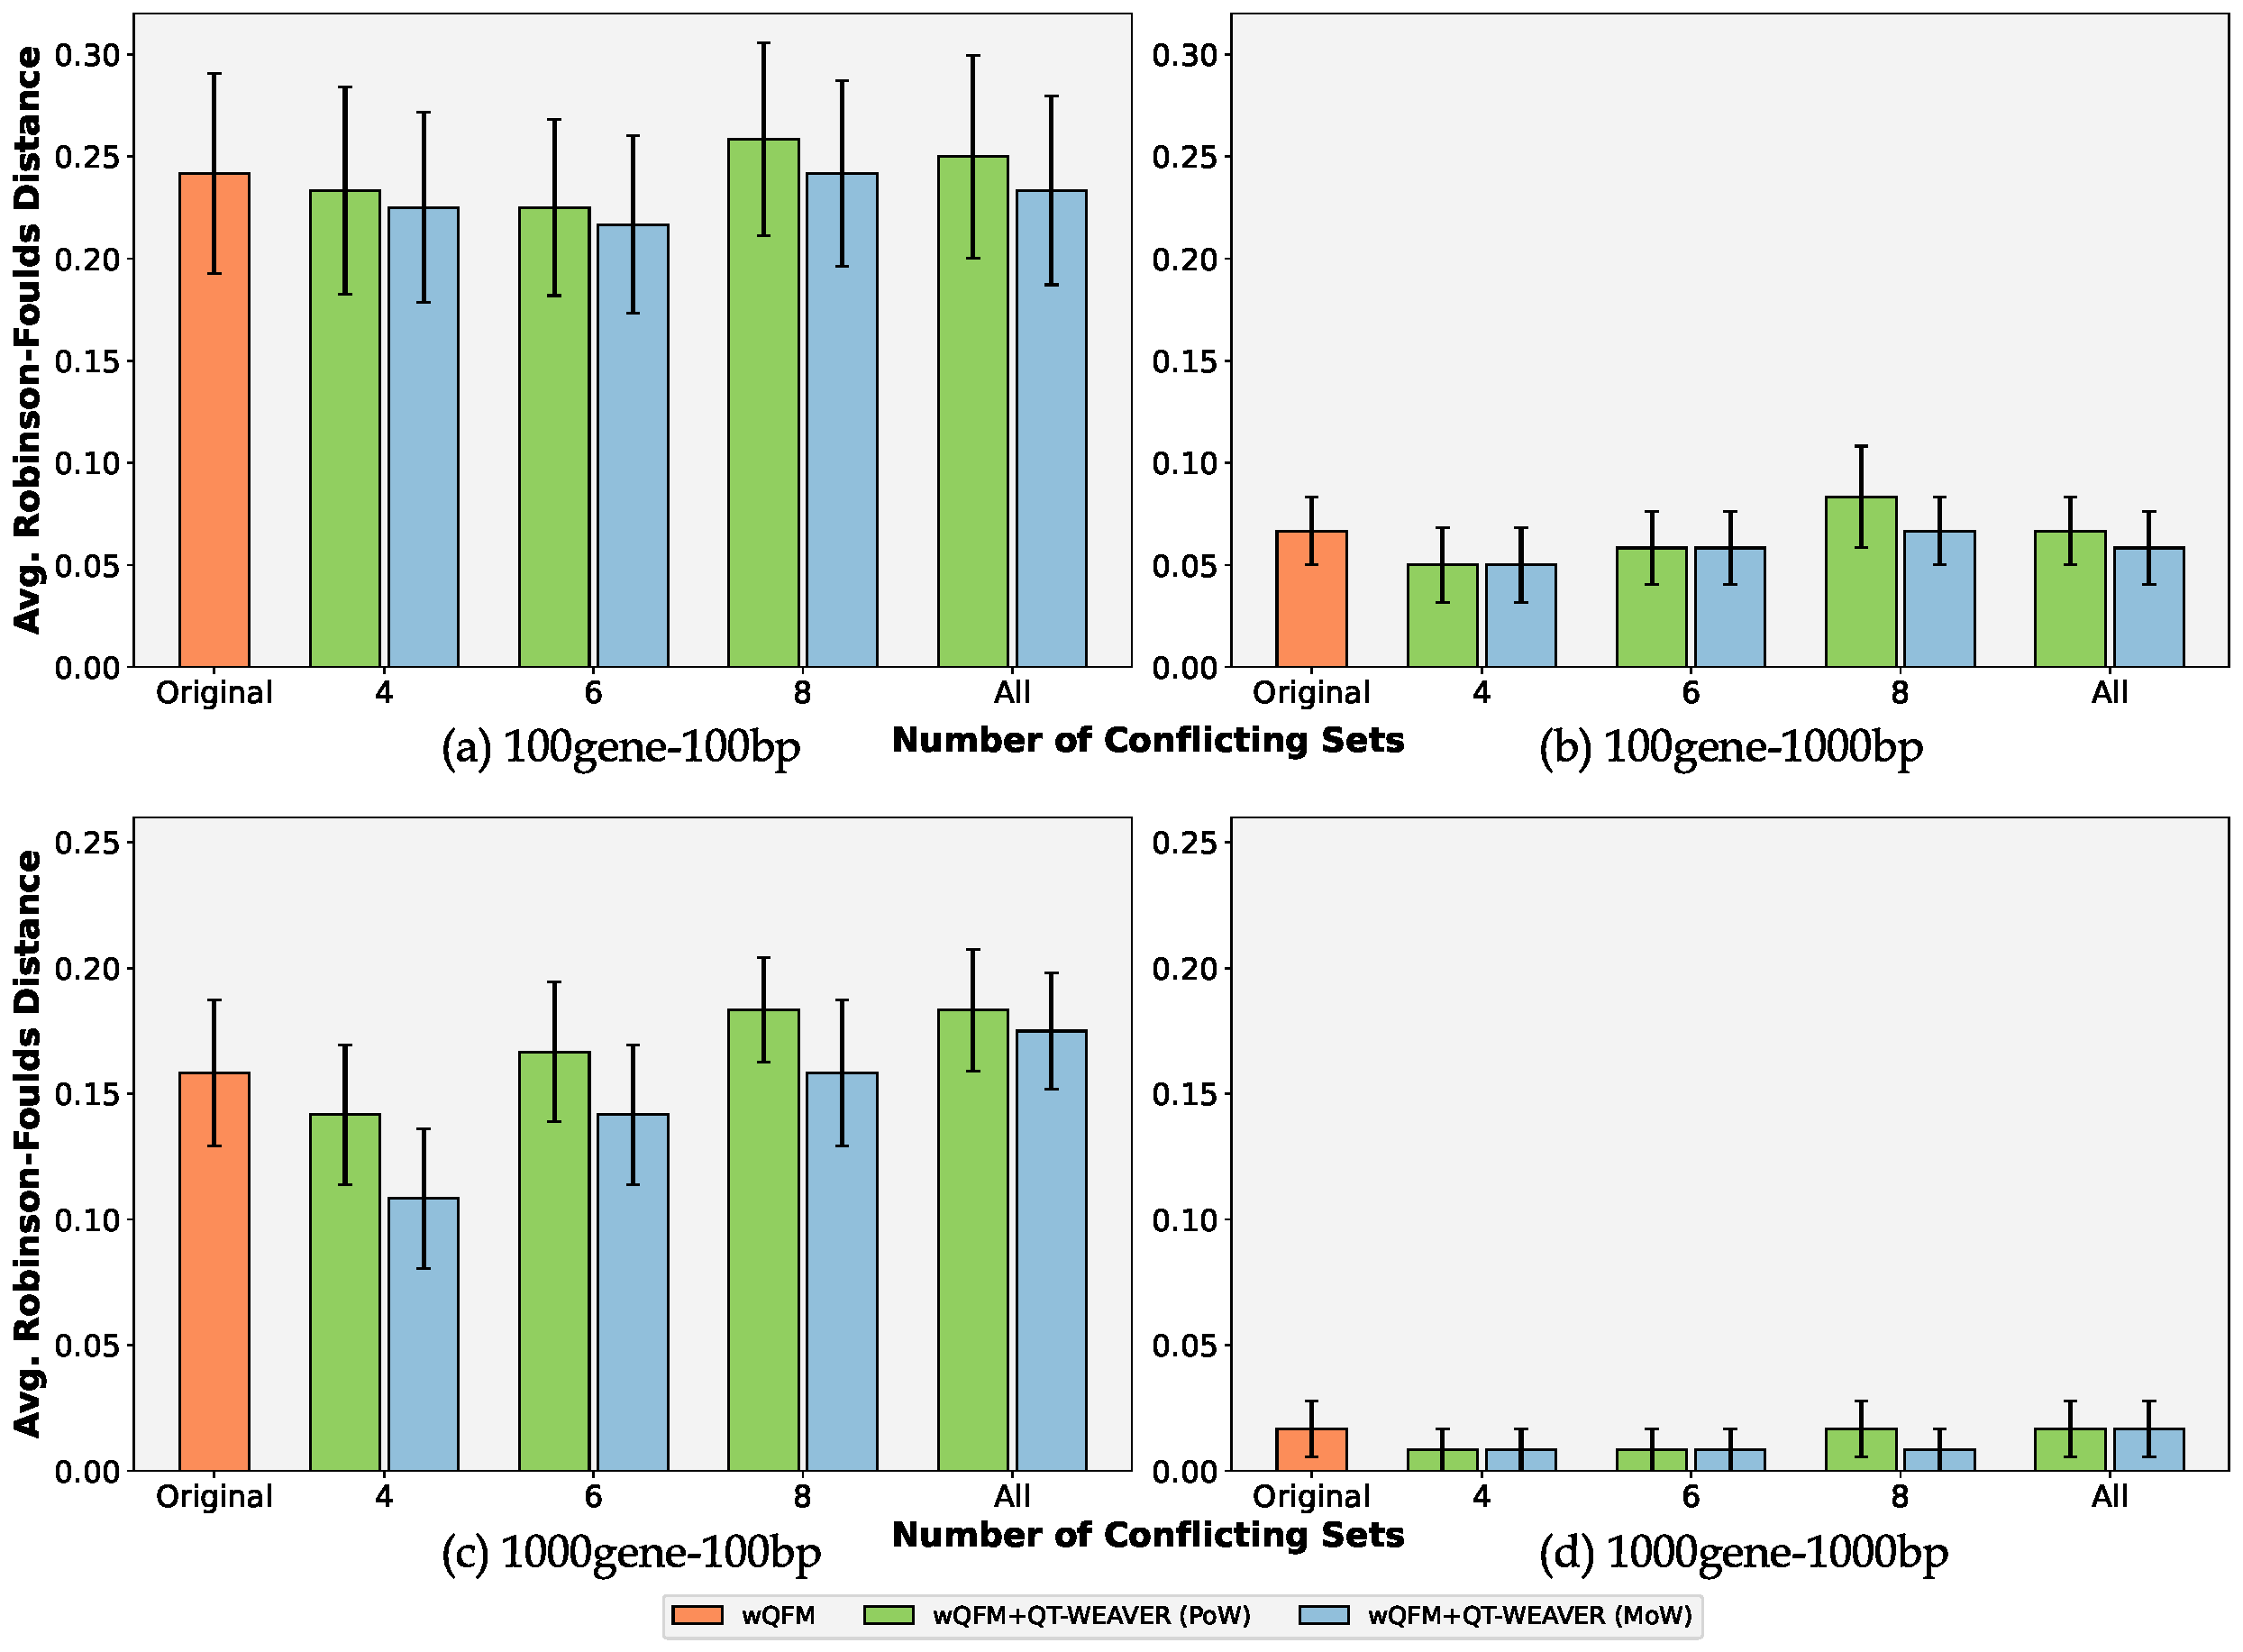
\includegraphics[width=\linewidth]{figures_new/1_15_modes.pdf}
    \caption{\textbf{Results on 15-taxon dataset.} Comparison of performance after correcting the weighted distributions using four, six, eight, and all 28 conflicting sets. We report the RF rates averaged over 10 replicates with standard errors. The distributions were amalgamated using wQFM. We show the effects of using both PoW and MoW weighting schemes. }
    \label{fig:rf_15_taxon_schemes}
\end{figure}

These results raise the question -- why does considering a small subset of all conflicting sets tend to yield better results? We hypothesize that using all 28 conflicting sets may impose excessive topological constraints on a quartet, making it challenging for QT-WEAVER to effectively distinguish among different topological variants.

In contrast, the six selected conflicting sets (as listed in Table \ref{table:conflicttable_six}) appear suitable for assessing conflict levels across quartet topologies, as indicated by our experimental results. While this specific choice of six sets lacks theoretical backing, we anticipate that the optimal subset--both in size and composition--may vary by dataset. Thus, an important research avenue involves automating the selection of these subsets, tailored to the topological features of the input gene trees, to optimize performance.

\begin{table}[h!]
    \centering
     \renewcommand{\arraystretch}{1.2}
    \begin{tabular}{|c|c|}
        \hline
        \textbf{Canonical Pair} & \textbf{Conflicting Quartets} \\ \hline

        $ab|cd$ \& $ac|be$ 
        & $ab|de$ $||$ $ae|bd$\\ \hline

        $ab|cd$ \& $ae|bc$ 
        & $ad|be$\\ \hline

        $ab|cd$ \& $ac|de$ 
        & $bd|ce$ $||$ $be|cd$\\ \hline

        $ab|cd$ \& $ad|ce$ 
        & $bc|de$\\ \hline
        
    \end{tabular}
    \caption{We list the six conflicting sets chosen from all the conflicting sets from Table \ref{table:conflicttable}.}
    \label{table:conflicttable_six}
\end{table}

%So, why is it that only considering a small subset of all conflicting sets tends to yield better results? We hypothesize that all 28 conflicting sets together might be enforcing too much topological constraint on a quartet. As a result, it becomes difficult for QT-WEAVER to differentiate very well between different topological variants.


%On the other hand, the six conflicting sets that we chose (as outlined in Table \ref{table:conflicttable_six}) seem to be appropriate for identifying the degree of conflicts for different quartet topologies (as demonstrated in our experiments). The choice of these exact six sets does not hold much theoretical ground (future studies need to investigate this), and -- we believe -- depending on the dataset, the optimal choice (both size and elements) may vary. Therefore, automatic selection of the size and elements of these subsets, based on the topological structures of the input gene trees, to optimize the results is an important research direction.


%The ``minimum" weighting scheme outperforms the "regular" weighting scheme on all occasions. Furthermore, considering four or six conflicting sets produces the best results; the set of all 28 conflicting sets yields decent species trees, too. 
%In the most difficult model condition (100gene-100bp), taking six conflicting sets turns out to be the best choice.

%As utilizing six conflicting sets is not only faster than considering all but also yields better performance across all model conditions, we will only use this method in subsequent analyses. Moreover, we will only use the ``minimum" weighting scheme due to its superiority over the ``regular" weighting scheme. From now on, ``wQFM + QT-WEAVER" will denote estimating trees using wQFM on distributions corrected by QT-WEAVER with the minimum weighting scheme using six conflicting sets.


\section{Dataset}
\label{app:dataset}

\begin{table}[htbp]
\caption{Properties of the simulated datasets. The level of ILS is presented in terms of the average topological distance between true gene trees and true species trees.}
\label{table.data-description}
\centering
\begin{tabular}{c c c c c c} 
 \hline
 Dataset & ILS level & \# genes & \# sites & \# Replicates & Ref.\\  [0.5ex]
 \hline\hline
% 10-taxon & 40\%, 84\% & 200 & 100 & 20 & \cite{bayzid2015weighted} \\
% \hline
% 11-taxon & 38\%, 85\% & 5 - 100 & 2000 & 20 & \cite{chung2011} \\
 %\hline
 15-taxon & 82\% & 100 - 1000 & 100 - 1000 & 10 & \cite{bayzid2015weighted}\\
 \hline
 37-taxon & 18\%, 32\%, 54\% & 100 - 500 & 50 -1000 & 20 & \cite{statistical-binning}\\
 \hline
 
\end{tabular}
\end{table}

%\clearpage
\section{Additional Results}
\label{app:additional-results}

\subsection{Additional results on 37-taxon dataset}
\label{app:37-taxon}

\begin{table}[h!]
    \centering
    % \small
    % \tiny
    \caption{The Jensen-Shannon divergence with respect to the true gene trees for different model conditions averaged over all replicates. The best-performing method (i.e., the least amount of divergence) for each model condition has been highlighted in bold.}
    % \bigskip
    \label{tab:37-divergence}
    \begin{tabular}{|C{3cm}|C{3cm}|C{3cm}|}
        \hline
        \textbf{Model Condition} & \textbf{GTF} & \textbf{QT-WEAVER} \\
        \hline
        0.5X-200-500 & \textbf{0.038} & 0.044 \\
        \hline
        1X-100-500 & 0.072 & \textbf{0.067} \\
        \hline
        1X-200-25 & 0.354 & \textbf{0.345} \\
        \hline
        1X-200-50 & 0.3 & \textbf{0.287} \\
        \hline
        1X-200-250 & 0.118 & \textbf{0.097} \\
        \hline
        1X-200-500 & 0.063 & \textbf{0.058} \\
        \hline
        1X-200-1000 & \textbf{0.034} & 0.053 \\
        \hline
        1X-500-500 & 0.057 & \textbf{0.052} \\
        \hline
        2X-200-500 & 0.097 & \textbf{0.082} \\
        \hline
    \end{tabular}
\end{table}

\begin{table}[h!]
    \centering
    % \small
    % \tiny
    \caption{Average quartet scores of estimated species trees and the true tree with respect to the estimated gene trees for the 37-taxon dataset. For wQFM+QT-WEAVER, we also report the quartet score with respect to the corrected estimated quartet distribution. The highest scores among the estimated trees have been italicized, and the scores closest to the true tree are shown in bold.}
    % \bigskip
    \label{tab:37-quartet-scores-estimated}
    \begin{tabular}{|C{2cm}|C{2.5cm}|C{2.5cm}|C{2.5cm}|C{2.5cm}|C{2.5cm}|}
        \hline
        \textbf{Model Condition} & \textbf{ASTRAL} & \textbf{wQFM} & \textbf{wQFM+QT-WEAVER (Original Distribution)} & \textbf{wQFM+QT-WEAVER (Corrected Distribution)} & \textbf{True Tree} \\
        \hline \hline
        0.5X-200-500 & 10007426 & 10006594 & \textbf{10006474} & \textit{10415670} & 10003930 \\
        \hline
        1X-100-500 & 5640132 & 5639605 & \textbf{5639168} & \textit{5806039} & 5636884 \\
        \hline
        1X-200-25 & 6491920 & 6489889 & \textbf{6489155} & \textit{6662792} & 6481431 \\
        \hline
        1X-200-50 & 7525465 & \textbf{7523379} & 7523903 & \textit{7778394} & 7517956 \\
        \hline
        1X-200-250 & 10569844 & 10568958 & \textbf{10568350} & \textit{10941339} & 10565292 \\
        \hline
        1X-200-500 & 11271938 & 11271426 & \textbf{11270680} & \textit{11603816} & 11267991 \\
        \hline
        1X-200-1000 & 11586641 & 11586355 & \textbf{11585945} & \textit{11886743} & 11584970 \\
        \hline
        1X-500-500 & 28171698 & \textbf{28171682} & 28168879 & \textit{28983587} & 28171386 \\
        \hline
        2X-200-500 & 11947266 & \textbf{11947020} & 11945419 & \textit{12175146} & 11946371 \\
        \hline
    \end{tabular}
\end{table}


\begin{table}[h!]
    \centering
    % \small
    % \tiny
    \caption{Average quartet scores of estimated species trees and the true tree with respect to the true gene trees for the 37-taxon dataset. The highest scores among the estimated trees have been italicized, and the scores closest to the true tree are shown in bold. %\add{Unlike Table \ref{tab:37-quartet-scores-estimated}, we could not report scores with respect to the corrected distribution, as we did not correct the true distribution (it has no GTEE).} \addb{But, didn't we show it in Figure \ref{fig:rf_37_taxon_methods}(c)?}
    }
    % \bigskip
    \label{tab:37-quartet-scores-true}
    \begin{tabular}{|C{2.3cm}|C{3cm}|C{3cm}|C{3cm}|C{3cm}|}
        \hline
        \textbf{Model Condition} & \textbf{ASTRAL} & \textbf{wQFM} & \textbf{wQFM+QT-WEAVER} & \textbf{True Tree} \\
        \hline \hline
        0.5X-200-500 & \textbf{\textit{10311630}} & 10311452 & 10311480 & 10311622 \\
        \hline
        1X-100-500 & 5870845 & 5871208 & \textbf{\textit{5871324}} & 5874698 \\
        \hline
        1X-200-25 & \textbf{\textit{11637683}} & 11613065 & 11627649 & 11744079 \\
        \hline
        1X-200-50 & 11688779 & \textbf{\textit{11707476}} & 11703316 & 11744079 \\
        \hline
        1X-200-250 & 11733853 & \textbf{\textit{11735693}} & 11731082 & 11744079 \\
        \hline
        1X-200-500 & 11738631 & 11739572 & \textbf{\textit{11741356}} & 11744079 \\
        \hline
        1X-200-1000 & 11743809 & 11743721 & \textbf{\textit{11744134}} & 11744079 \\
        \hline
        1X-500-500 & 29362939 & \textbf{\textit{29363114}} & 29356078 & 29364014 \\
        \hline
        2X-200-500 & 12565282 & \textbf{\textit{12565347}} & 12563879 & 12570343 \\
        \hline
    \end{tabular}
\end{table}


\begin{figure}[h]
    \centering % <-- added
    % 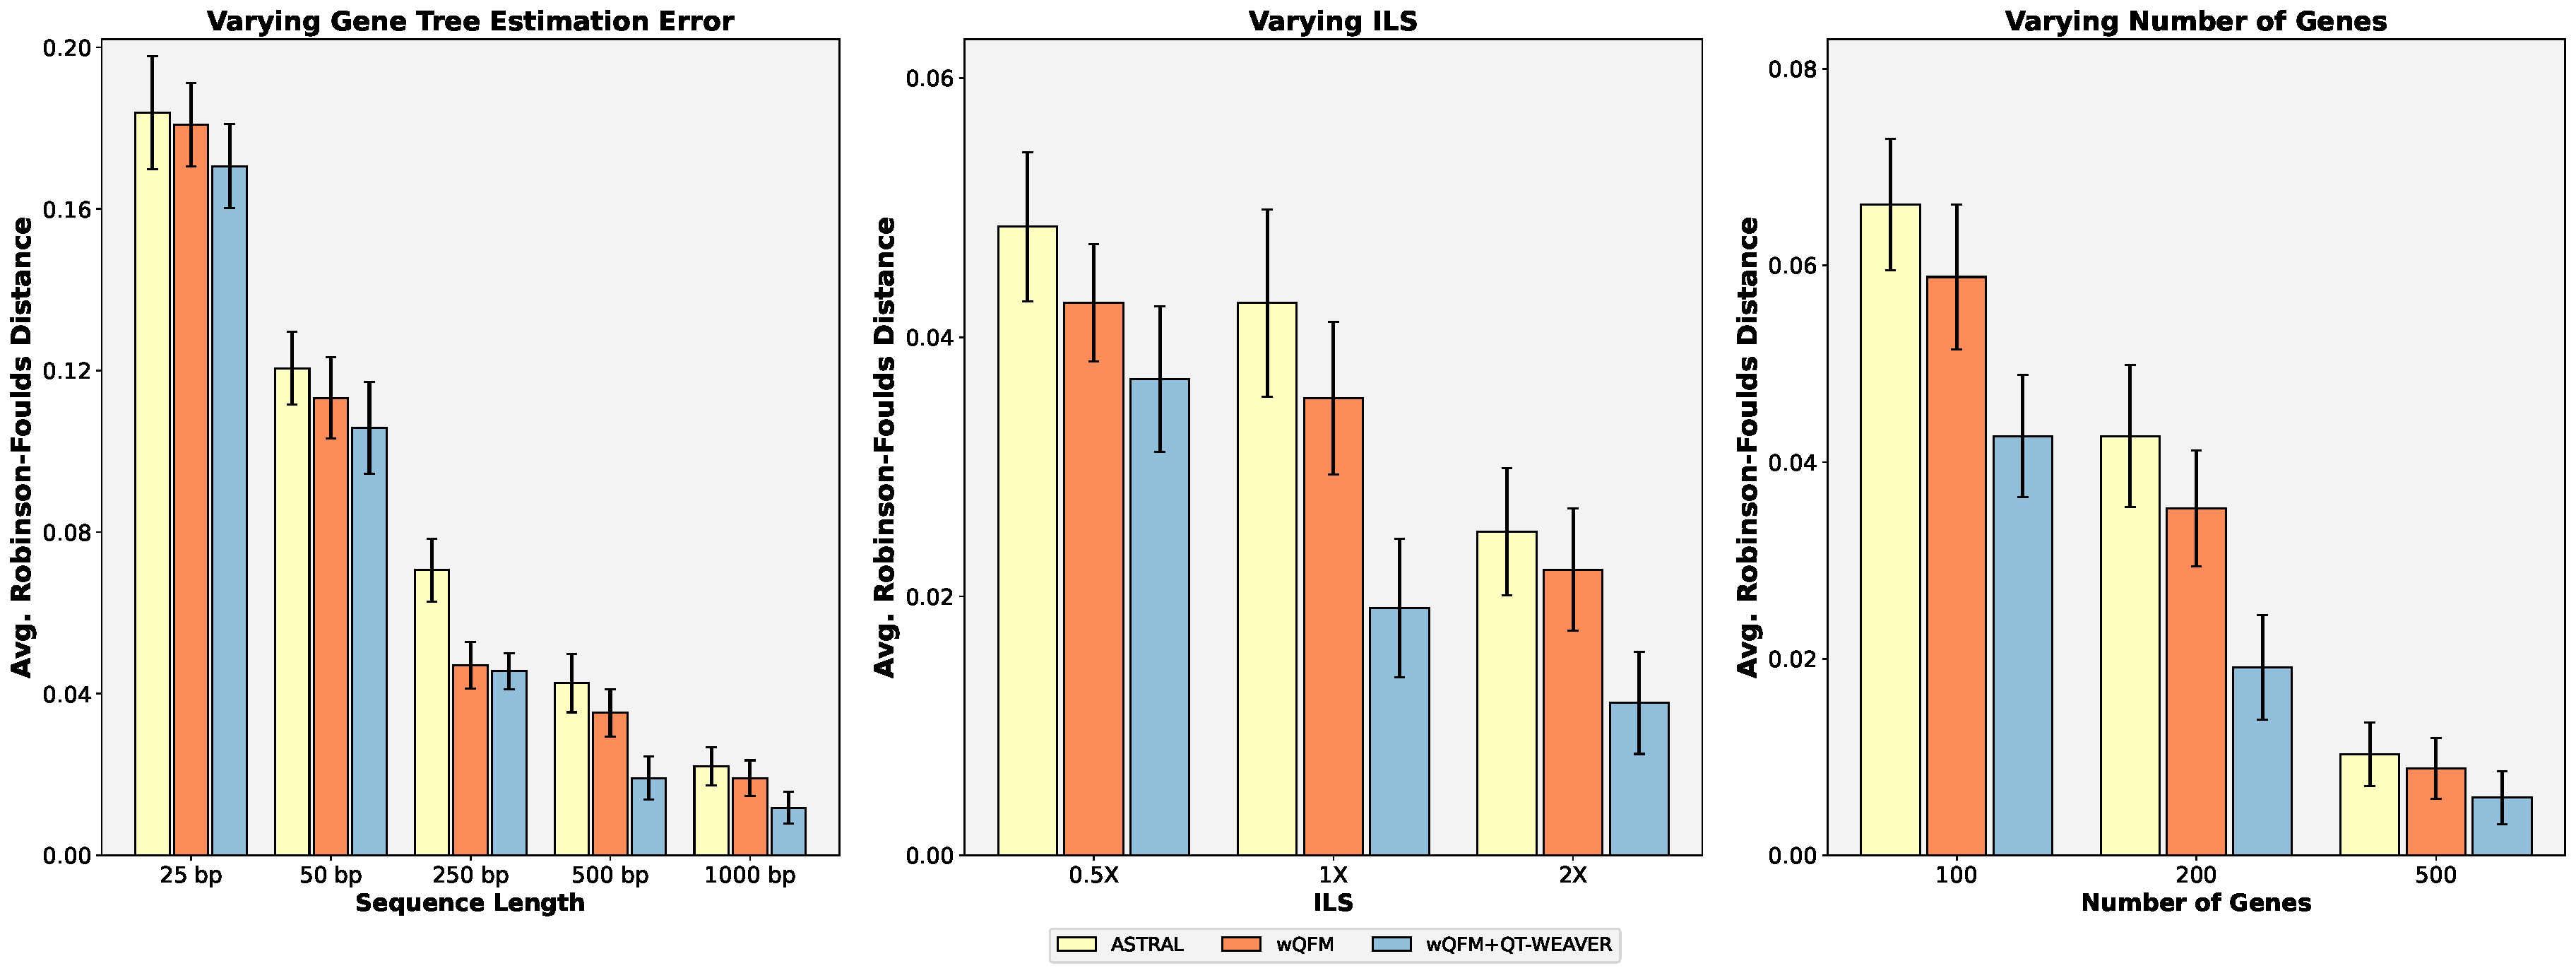
\includegraphics[width=\linewidth]{figures_new/2_37_methods.pdf}
    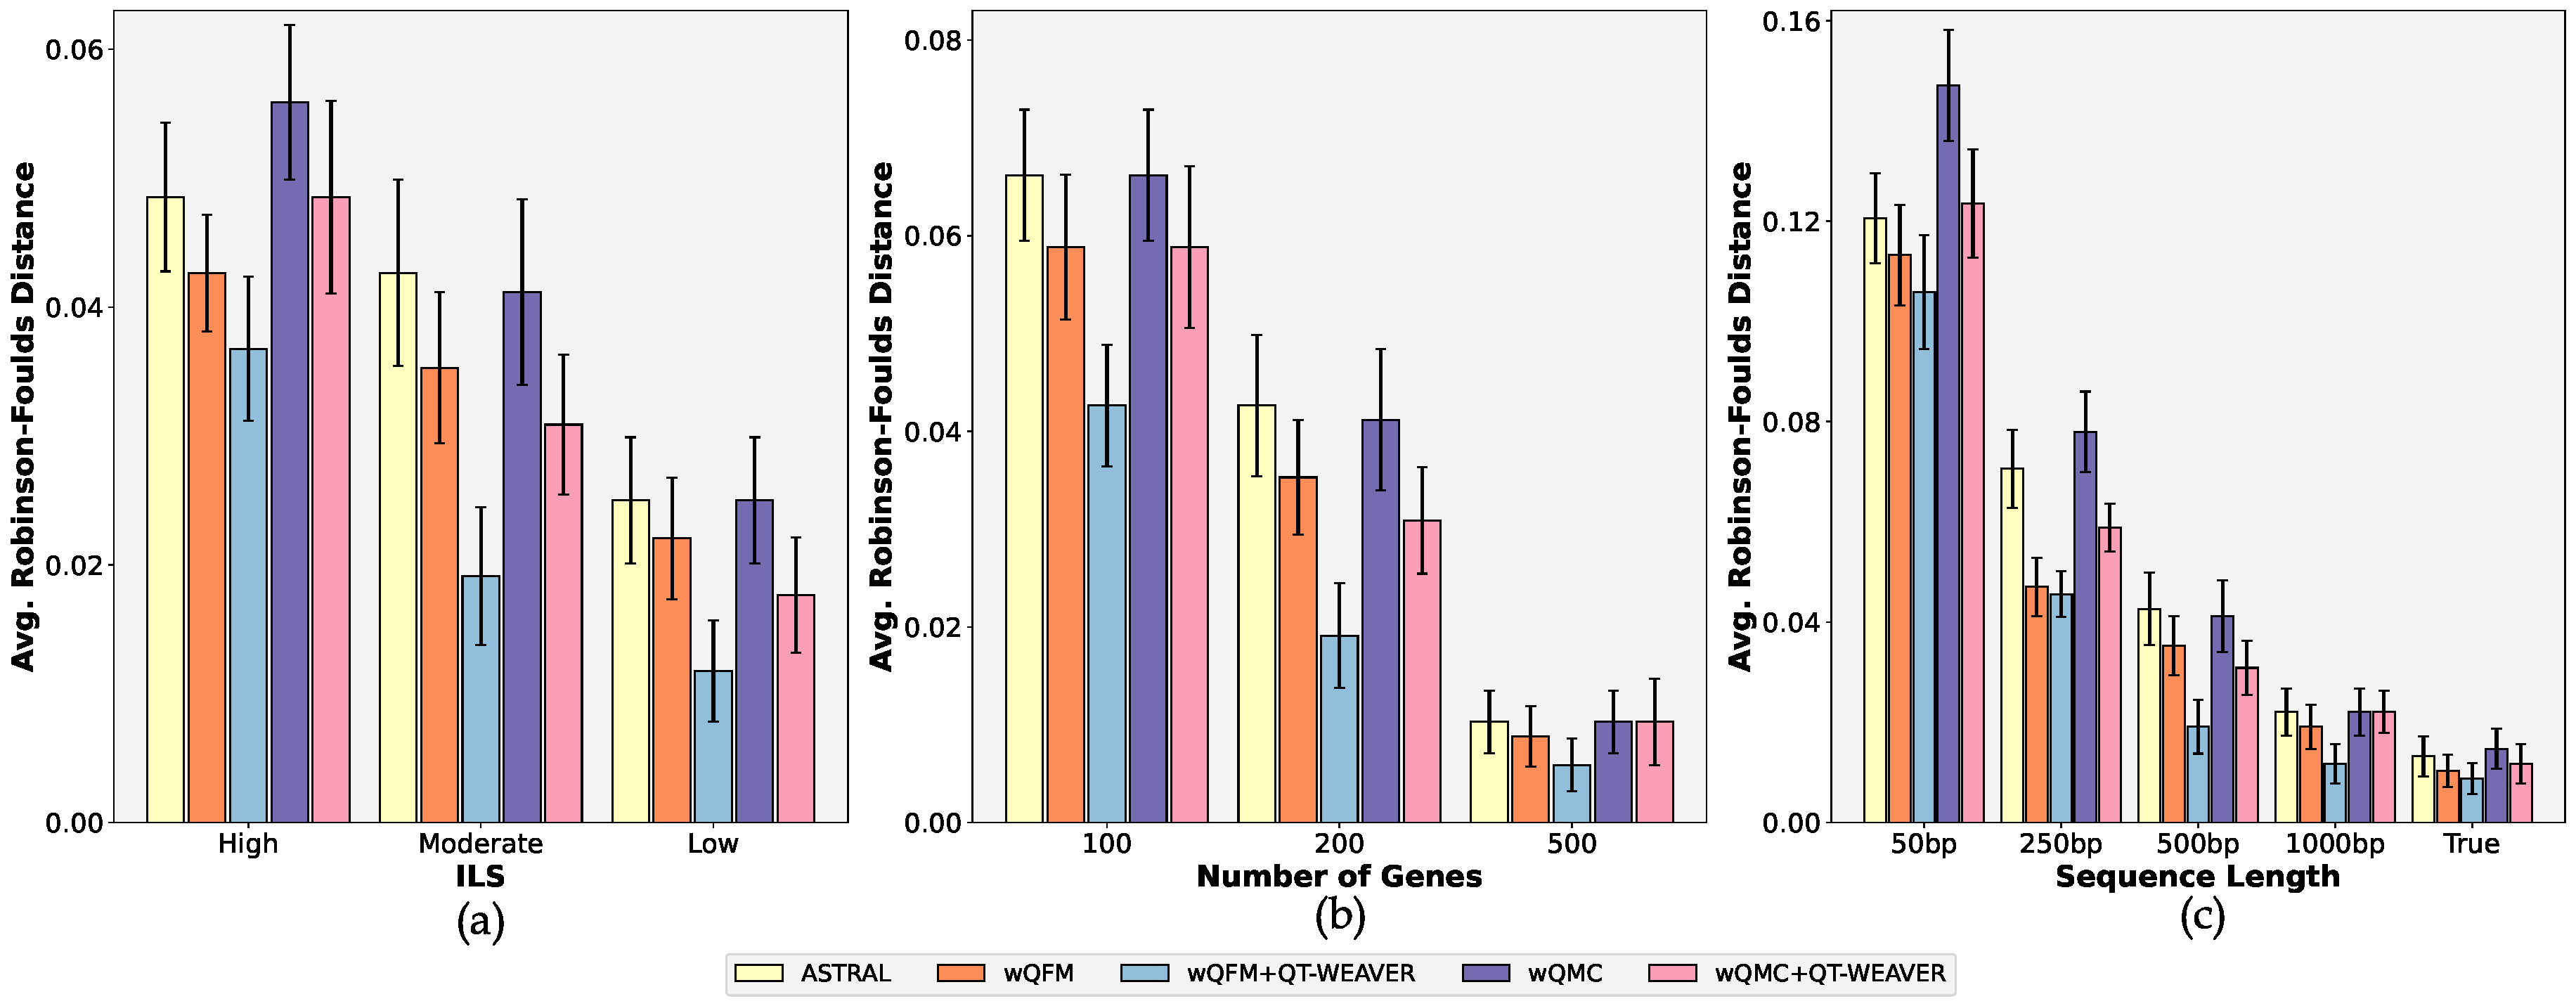
\includegraphics[width=\linewidth]{figures_new/9_37_methods_wqmc.pdf}
    \caption{\textbf{Results on 37-taxon dataset.} We show the average RF rates with standard errors over 20 replicates for the methods ASTRAL, wQFM (wQFM-uncorrected), wQFM+QT-WEAVER (wQFM-corrected), wQMC (wQMC-uncorrected), and wQMC+QT-WEAVER (wQMC-corrected). The settings in (a)-(c) are identical to the ones in Figure \ref{fig:rf_37_taxon_methods}. }
    \label{fig:rf_37_taxon_wqmc}
\end{figure}

\newpage

\subsection{Additional results on 15-taxon dataset}
\label{app:15-taxon}

% \begin{figure}[h!]
%     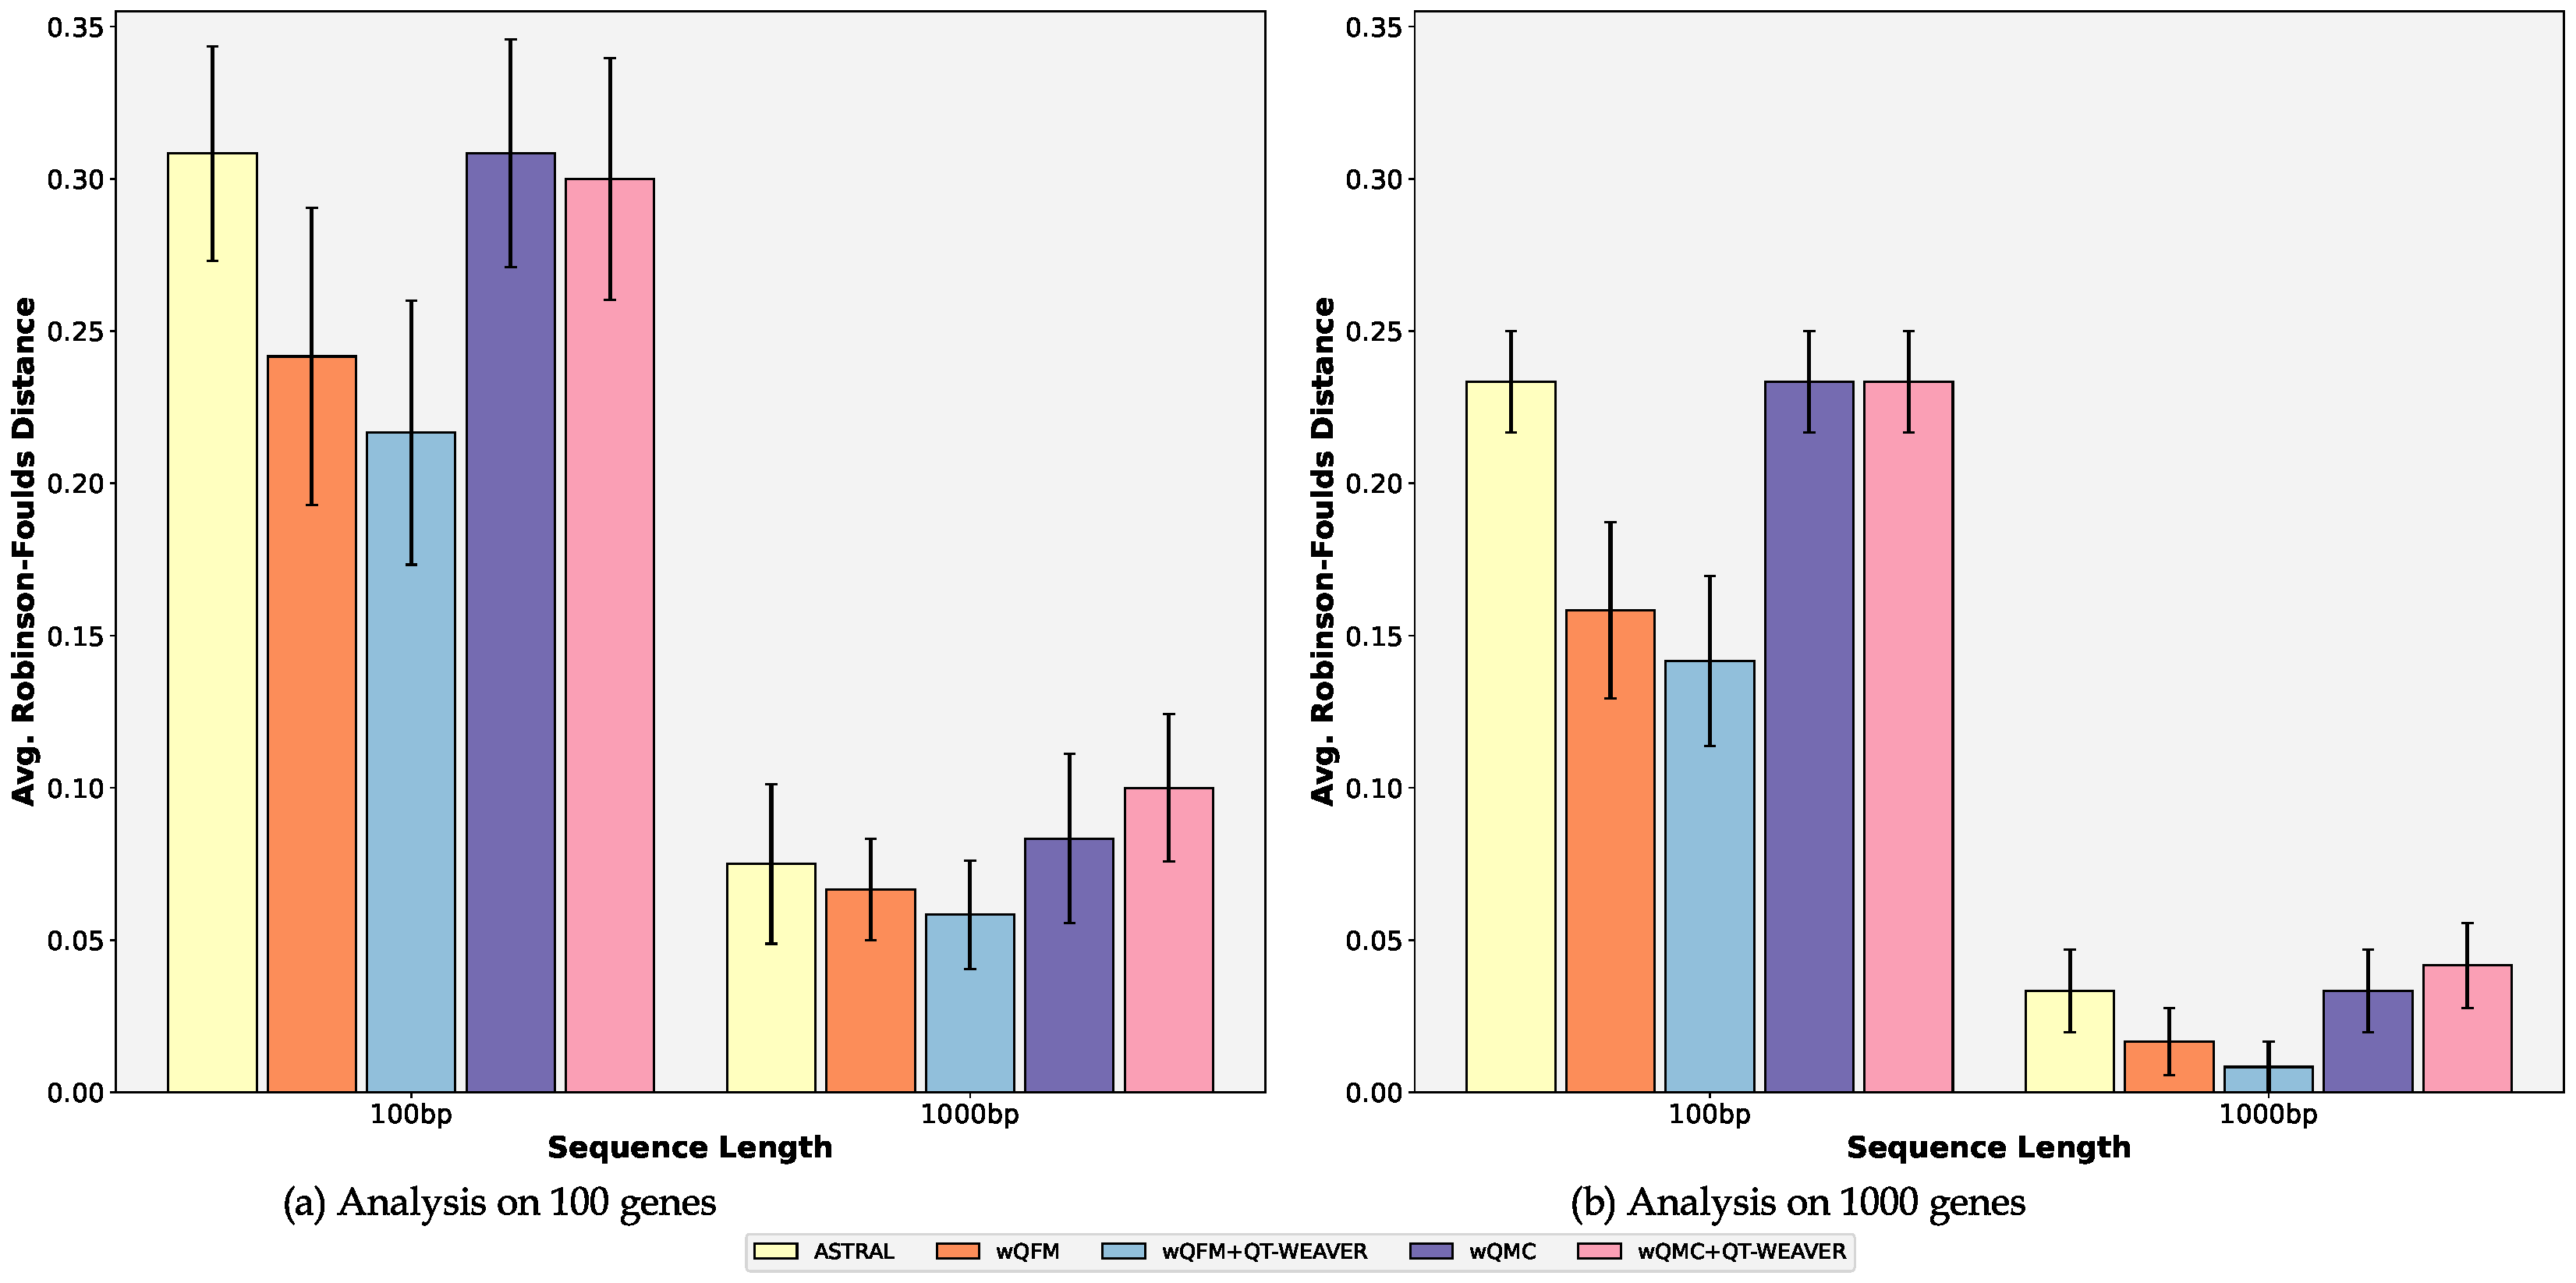
\includegraphics[width=\linewidth, height=0.5\linewidth]{figures_new/9_15_methods_wqmc.pdf}
%     \caption{\textbf{Results on 15-taxon dataset.} (a)-(b) We compare the average RF distance of ASTRAL, wQFM, wQFM+QT-WEAVER, wQMC, and wQMC+QT-WEAVER on varying model conditions. The settings are identical to the ones in Figure \ref{fig:rf_15_taxon_methods}.}
%     \label{fig:rf_15_taxon_methods_wqmc}
% \end{figure}


\begin{table}[h!]
    \centering
    % \small
    % \tiny
    \caption{The Jensen-Shannon divergence with respect to the true gene trees for different model conditions averaged over all replicates. The best-performing method (i.e., the least amount of divergence) for each model condition has been highlighted in bold.}
    % \bigskip
    \label{tab:15-divergence}

    \begin{tabular}{|c|C{3cm}|C{3cm}|}
        \hline
        \textbf{Model Condition} & \textbf{GTF} & \textbf{QT-WEAVER} \\
        \hline
        100gene-100bp & 0.115 & \textbf{0.103} \\
        \hline
        100gene-1000bp & \textbf{0.043} & 0.049 \\
        \hline
        1000gene-100bp & 0.101 & \textbf{0.087} \\
        \hline
        1000gene-1000bp & \textbf{0.031} & 0.037 \\
        \hline
    \end{tabular}
\end{table}

\begin{table}[h!]
    \centering
    % \small
    % \tiny
    \caption{Average quartet scores of estimated species trees and the true tree with respect to the estimated gene trees for the 15-taxon dataset. For wQFM+QT-WEAVER, we also report the quartet score with respect to the corrected estimated quartet distribution. The highest scores among the estimated trees have been italicized, and the scores closest to the true tree are shown in bold.}
    % \bigskip
    \label{tab:15-quartet-scores-estimated}
    \begin{tabular}{|C{2cm}|C{2.5cm}|C{2.5cm}|C{2.5cm}|C{2.5cm}|C{2.5cm}|}
        \hline
        \textbf{Model Condition} & \textbf{ASTRAL} & \textbf{wQFM} & \textbf{wQFM+QT-WEAVER (Original Distribution)} & \textbf{wQFM+QT-WEAVER (Corrected Distribution)} & \textbf{True Tree} \\
        \hline \hline
        100gene-100bp & 69934 & \textbf{69777} & 69792 & \textit{73598} & 69307 \\
        \hline
        100gene-1000bp & 82167 & 82129 & \textbf{82125} & \textit{87562} & 82099 \\
        \hline
        1000gene-100bp & 693656 & 692949 & \textbf{692664} & \textit{727712} & 690268 \\
        \hline
        1000gene-1000bp & 818022 & 817994 & \textbf{817953} & \textit{869904} & 817937 \\
        \hline
    \end{tabular}
\end{table}

\begin{table}[h!]
    \centering
    % \small
    % \tiny
    \caption{Average quartet scores of estimated species trees and the true tree with respect to the true gene trees for the 15-taxon dataset. The highest scores among the estimated trees have been italicized, and the scores closest to the true tree are shown in bold.}
    % \bigskip
    \label{tab:15-quartet-scores-true}
    \begin{tabular}{|C{2.3cm}|C{3cm}|C{3cm}|C{3cm}|C{3cm}|}
        \hline
        \textbf{Model Condition} & \textbf{ASTRAL} & \textbf{wQFM} & \textbf{wQFM+QT-WEAVER} & \textbf{True  Tree} \\
        \hline \hline
        100gene-100bp & 82159 & 82708 & \textbf{\textit{83078}} & 84635 \\
        \hline
        100gene-1000bp & 84345 & 84437 & \textbf{\textit{84444}} & 84635 \\
        \hline
        1000gene-100bp & 827970 & 834890 & \textbf{\textit{836349}} & 844184 \\
        \hline
        1000gene-1000bp & 843363 & 843792 & \textbf{\textit{843973}} & 844184 \\
        \hline
    \end{tabular}
\end{table}

%On the other hand, maximizing the quartet scores with respect to the estimated gene trees may not guarantee more accuracy in the presence of gene tree estimation errors and limited number of genes. The true tree having the lowest quartet scores across all model conditions supports this claim (Table \ref{tab:15-quartet-scores-estimated}). ASTRAL attains the highest quartet scores, which is furthest from the true tree, suggesting that it is ``overshooting" the quartet scores as it returns the least accurate tree among the three methods. Clearly, the wQFM+QT-WEAVER species trees, when compared to the original estimated distribution, are suffering from this ``overshooting" issue the least, which results in the best trees. Interestingly, when we consider the ``corrected" estimated distribution, the quartet scores of wQFM+QT-WEAVER are by far the highest, indicating that the corrected distribution was able to shed much of the limitations caused by gene tree estimation error and a limited number of genes. Hence, the corrected distribution is a more reliable representation of the true distribution.

% \newpage
\clearpage

\subsection{Additional results on iterative corrections using QT-WEAVER}
\label{app:iterations}

We investigated how the Jensen-Shannon divergence evolves across iterations (see Figure \ref{fig:rf_15_taxon_iterative_2}(a) in Appendix \ref{app:iterations}). Initially, the divergence decreases during the first one or two iterations but then begins to increase. This occurs because, for the three alternative quartet topologies ($ab|cd, ac|bd, ad|bc$) on four taxa, QT-WEAVER tends to prioritize the quartet topology it identifies as ``correct'' --the one with the least conflict score--by increasing its weight while reducing the weights of the alternative topologies.  Thus, with successive iterations, the weight of the ``correct'' quartet topology continues to rise (toward 100\%) while the weights of the other two alternatives keep decreasing (toward 0\%). Thus, this overestimation of the weight of the ``correct'' quartets and the underestimation of the weights of the ``incorrect'' ones lead the adjusted distribution to diverge from the true weighted distribution. Despite this divergence, the iterative adjustments may still guide the tree search algorithm toward more accurate trees (up to a certain point) by emphasizing and amalgamating the quartets with higher weights, as evidenced by the gradual decrease in the RF rates up to 10-15 iterations. For the same reason, when examining the quartet scores of wQFM+QT-WEAVER with respect to the corresponding corrected quartet distribution (instead of the original quartet distribution), the scores continue to increase, approaching nearly 100\% (see Figure \ref{fig:rf_15_taxon_iterative_2}(b) in Appendix \ref{app:iterations}). This occurs because, in the corrected distribution, the weights of the quartets present in the estimated species trees steadily rise, resulting in higher quartet scores for the estimated trees.


\begin{figure}[h!]
    \centering % <-- added
    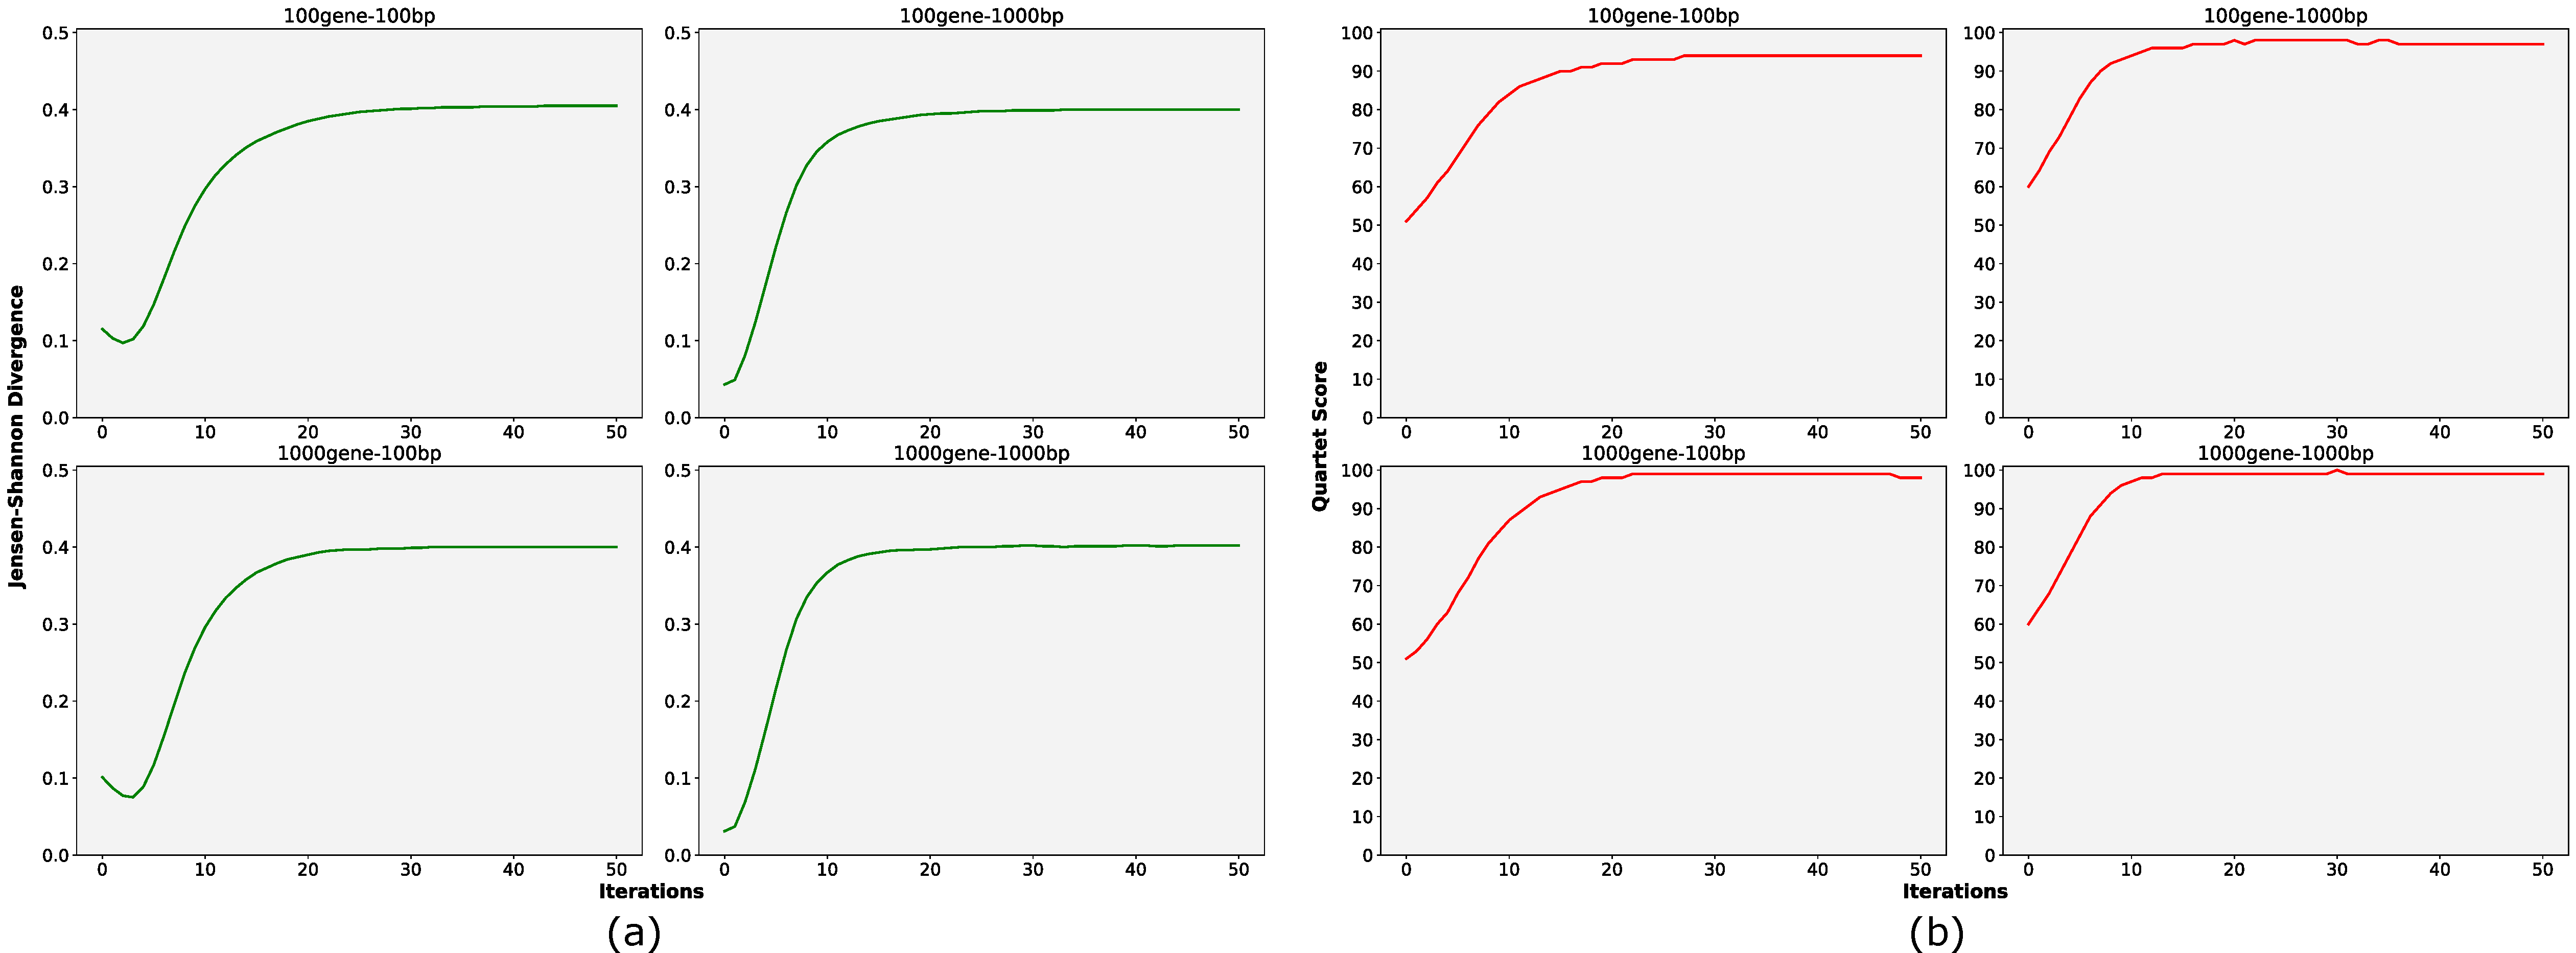
\includegraphics[width=\linewidth]{figures_new/15_iterative_2.pdf}
    \caption{\textbf{Results iterative corrections on 15-taxon dataset.} We show the changes in (a) Jensen-Shannon divergence with respect to the true quartet distribution and (b) the quartet score of the estimated species tree with respect to its corresponding corrected quartet distribution over 50 iterations. 
    }
    \label{fig:rf_15_taxon_iterative_2}
\end{figure}


% \subsection{Running time}
% \label{app:running-time}
% \begin{table}[htbp]
% \caption{Running time of QT-GILD for one epoch on different dataset.}
% \label{table.running time}
% \centering
% \begin{tabular}{c  c c } 
%  \toprule
%  Dataset &  \# Genes & Running time (seconds)  \\  [0.5ex]
%  \hline\hline
%  15-taxon & 100 & 25\times10^{-3} - 26\times10^{-3} \\
%  15-taxon & 1000 & 750\times10^{-3} - 800\times10^{-3} \\ \midrule
%  37-taxon & 100 & 1 $-$ 1.5\\
%  37-taxon & 200 & 2 $-$ 3\\
%  37-taxon & 400 & 5 $-$ 6\\ \midrule
%  Angiosperm (46-taxon) & 310 & 10 $-$ 11\\
%  \bottomrule
 
% \end{tabular}
% \end{table}

\newpage

\section{Analysis of Avian Biological Dataset}
\label{app:avian-biological}


\begin{figure}[h!]  
\centering
    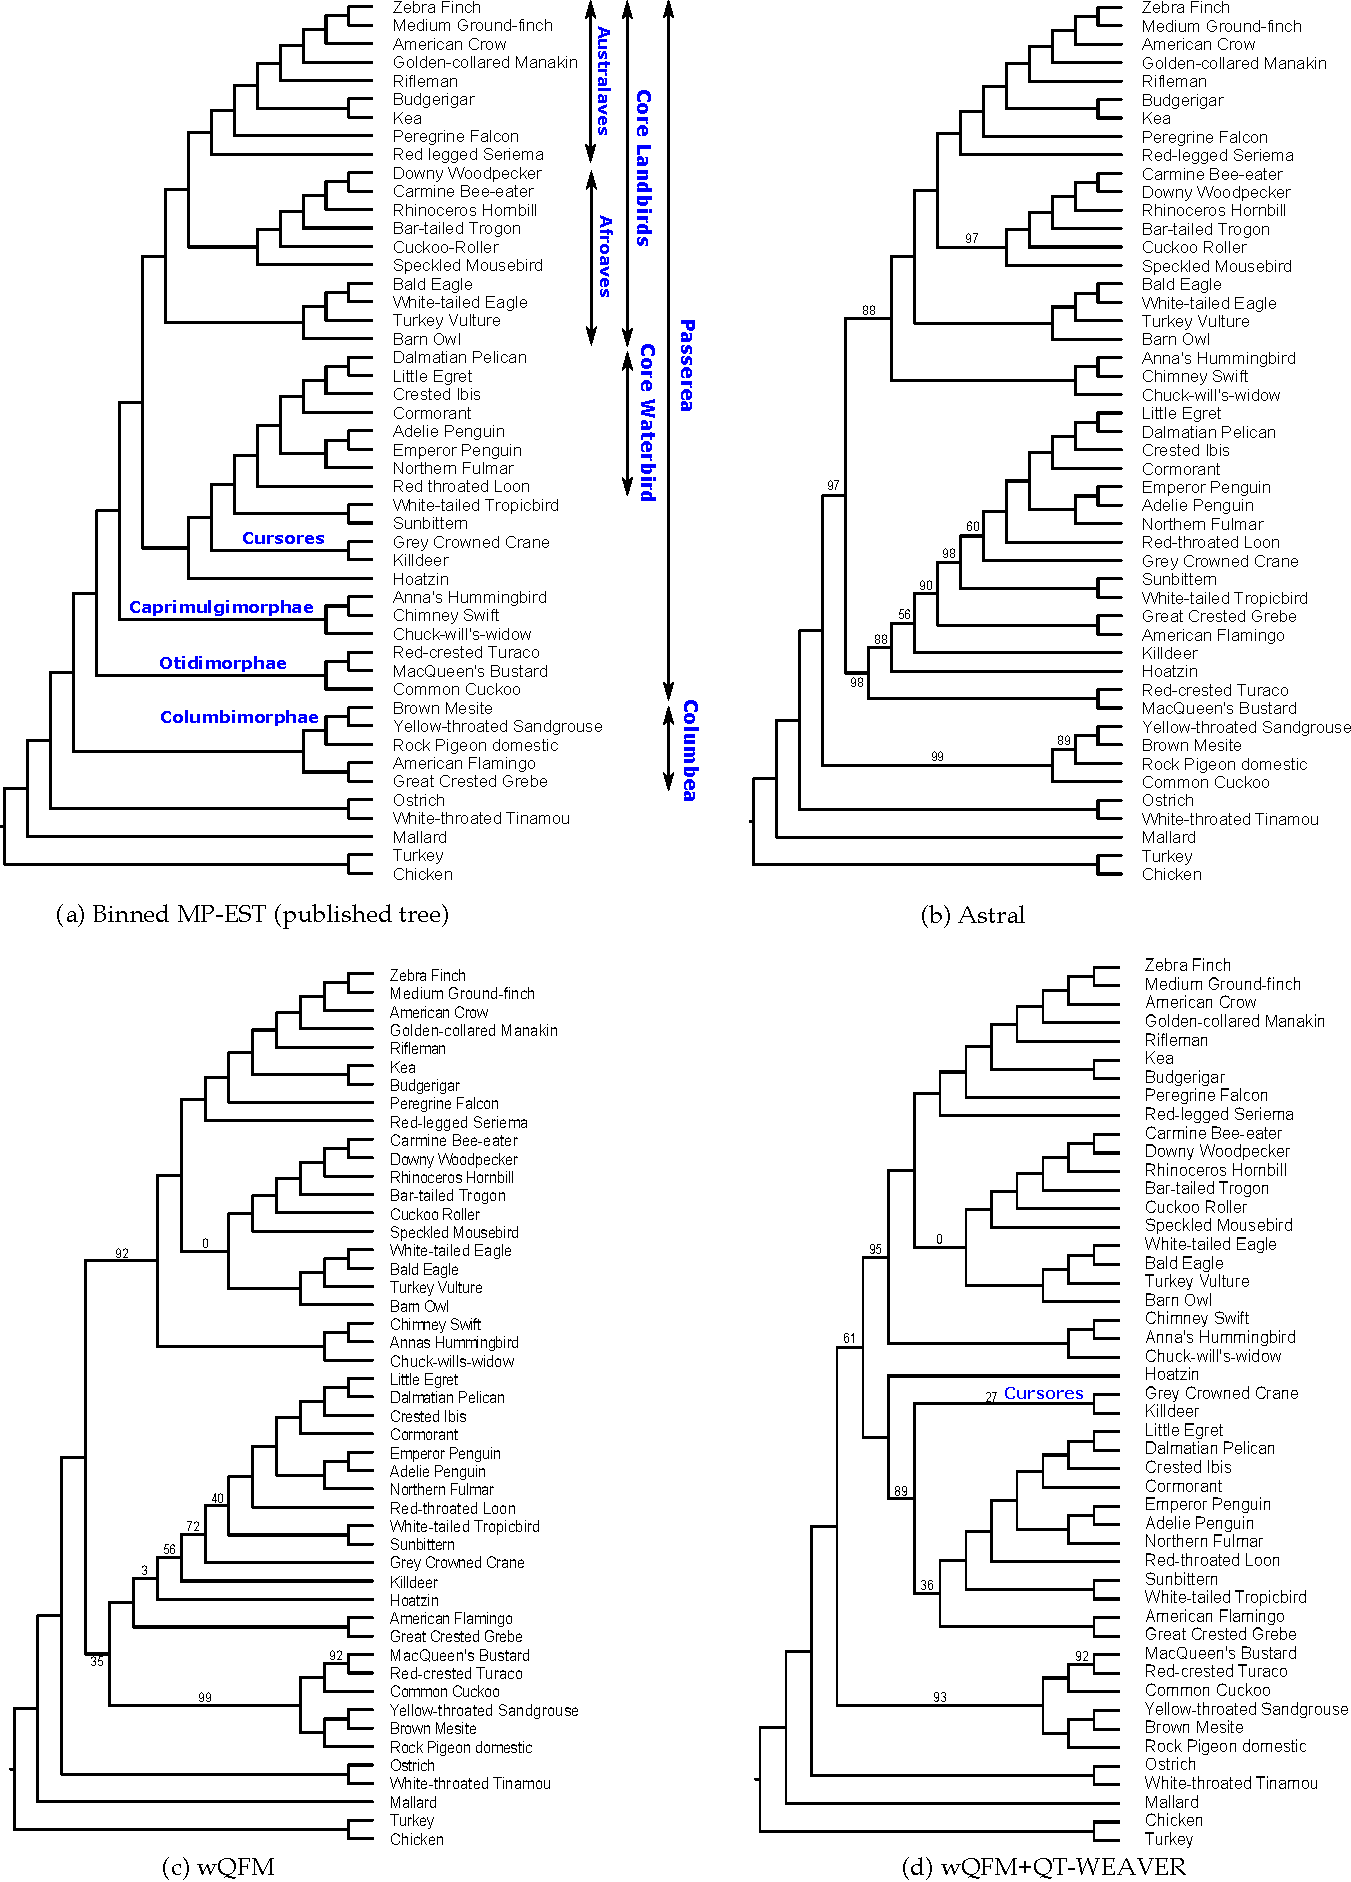
\includegraphics[width=0.85\linewidth]{figures_new/avian-combined-v2.pdf}
    \caption{\textbf{Analyses of the avian dataset using ASTRAL and wQFM (before and after correction).} 
    Branch supports are computed based on quartet-based local posterior probability~\cite{sayyari2016fast} (multiplied by 100). All BS values are 100\% except where noted.}
    \label{fig:avian}
\end{figure}


\end{appendices}
\end{document}
